\PassOptionsToPackage{unicode=true}{hyperref} % options for packages loaded elsewhere
\PassOptionsToPackage{hyphens}{url}
%
\documentclass[]{book}
\usepackage{lmodern}
\usepackage{amssymb,amsmath}
\usepackage{ifxetex,ifluatex}
\usepackage{fixltx2e} % provides \textsubscript
\ifnum 0\ifxetex 1\fi\ifluatex 1\fi=0 % if pdftex
  \usepackage[T1]{fontenc}
  \usepackage[utf8]{inputenc}
  \usepackage{textcomp} % provides euro and other symbols
\else % if luatex or xelatex
  \usepackage{unicode-math}
  \defaultfontfeatures{Ligatures=TeX,Scale=MatchLowercase}
\fi
% use upquote if available, for straight quotes in verbatim environments
\IfFileExists{upquote.sty}{\usepackage{upquote}}{}
% use microtype if available
\IfFileExists{microtype.sty}{%
\usepackage[]{microtype}
\UseMicrotypeSet[protrusion]{basicmath} % disable protrusion for tt fonts
}{}
\IfFileExists{parskip.sty}{%
\usepackage{parskip}
}{% else
\setlength{\parindent}{0pt}
\setlength{\parskip}{6pt plus 2pt minus 1pt}
}
\usepackage{hyperref}
\hypersetup{
            pdftitle={RJafroc Documentation},
            pdfauthor={Dev P. Chakraborty, PhD},
            pdfborder={0 0 0},
            breaklinks=true}
\urlstyle{same}  % don't use monospace font for urls
\usepackage{color}
\usepackage{fancyvrb}
\newcommand{\VerbBar}{|}
\newcommand{\VERB}{\Verb[commandchars=\\\{\}]}
\DefineVerbatimEnvironment{Highlighting}{Verbatim}{commandchars=\\\{\}}
% Add ',fontsize=\small' for more characters per line
\usepackage{framed}
\definecolor{shadecolor}{RGB}{248,248,248}
\newenvironment{Shaded}{\begin{snugshade}}{\end{snugshade}}
\newcommand{\AlertTok}[1]{\textcolor[rgb]{0.94,0.16,0.16}{#1}}
\newcommand{\AnnotationTok}[1]{\textcolor[rgb]{0.56,0.35,0.01}{\textbf{\textit{#1}}}}
\newcommand{\AttributeTok}[1]{\textcolor[rgb]{0.77,0.63,0.00}{#1}}
\newcommand{\BaseNTok}[1]{\textcolor[rgb]{0.00,0.00,0.81}{#1}}
\newcommand{\BuiltInTok}[1]{#1}
\newcommand{\CharTok}[1]{\textcolor[rgb]{0.31,0.60,0.02}{#1}}
\newcommand{\CommentTok}[1]{\textcolor[rgb]{0.56,0.35,0.01}{\textit{#1}}}
\newcommand{\CommentVarTok}[1]{\textcolor[rgb]{0.56,0.35,0.01}{\textbf{\textit{#1}}}}
\newcommand{\ConstantTok}[1]{\textcolor[rgb]{0.00,0.00,0.00}{#1}}
\newcommand{\ControlFlowTok}[1]{\textcolor[rgb]{0.13,0.29,0.53}{\textbf{#1}}}
\newcommand{\DataTypeTok}[1]{\textcolor[rgb]{0.13,0.29,0.53}{#1}}
\newcommand{\DecValTok}[1]{\textcolor[rgb]{0.00,0.00,0.81}{#1}}
\newcommand{\DocumentationTok}[1]{\textcolor[rgb]{0.56,0.35,0.01}{\textbf{\textit{#1}}}}
\newcommand{\ErrorTok}[1]{\textcolor[rgb]{0.64,0.00,0.00}{\textbf{#1}}}
\newcommand{\ExtensionTok}[1]{#1}
\newcommand{\FloatTok}[1]{\textcolor[rgb]{0.00,0.00,0.81}{#1}}
\newcommand{\FunctionTok}[1]{\textcolor[rgb]{0.00,0.00,0.00}{#1}}
\newcommand{\ImportTok}[1]{#1}
\newcommand{\InformationTok}[1]{\textcolor[rgb]{0.56,0.35,0.01}{\textbf{\textit{#1}}}}
\newcommand{\KeywordTok}[1]{\textcolor[rgb]{0.13,0.29,0.53}{\textbf{#1}}}
\newcommand{\NormalTok}[1]{#1}
\newcommand{\OperatorTok}[1]{\textcolor[rgb]{0.81,0.36,0.00}{\textbf{#1}}}
\newcommand{\OtherTok}[1]{\textcolor[rgb]{0.56,0.35,0.01}{#1}}
\newcommand{\PreprocessorTok}[1]{\textcolor[rgb]{0.56,0.35,0.01}{\textit{#1}}}
\newcommand{\RegionMarkerTok}[1]{#1}
\newcommand{\SpecialCharTok}[1]{\textcolor[rgb]{0.00,0.00,0.00}{#1}}
\newcommand{\SpecialStringTok}[1]{\textcolor[rgb]{0.31,0.60,0.02}{#1}}
\newcommand{\StringTok}[1]{\textcolor[rgb]{0.31,0.60,0.02}{#1}}
\newcommand{\VariableTok}[1]{\textcolor[rgb]{0.00,0.00,0.00}{#1}}
\newcommand{\VerbatimStringTok}[1]{\textcolor[rgb]{0.31,0.60,0.02}{#1}}
\newcommand{\WarningTok}[1]{\textcolor[rgb]{0.56,0.35,0.01}{\textbf{\textit{#1}}}}
\usepackage{longtable,booktabs}
% Fix footnotes in tables (requires footnote package)
\IfFileExists{footnote.sty}{\usepackage{footnote}\makesavenoteenv{longtable}}{}
\usepackage{graphicx,grffile}
\makeatletter
\def\maxwidth{\ifdim\Gin@nat@width>\linewidth\linewidth\else\Gin@nat@width\fi}
\def\maxheight{\ifdim\Gin@nat@height>\textheight\textheight\else\Gin@nat@height\fi}
\makeatother
% Scale images if necessary, so that they will not overflow the page
% margins by default, and it is still possible to overwrite the defaults
% using explicit options in \includegraphics[width, height, ...]{}
\setkeys{Gin}{width=\maxwidth,height=\maxheight,keepaspectratio}
\setlength{\emergencystretch}{3em}  % prevent overfull lines
\providecommand{\tightlist}{%
  \setlength{\itemsep}{0pt}\setlength{\parskip}{0pt}}
\setcounter{secnumdepth}{5}
% Redefines (sub)paragraphs to behave more like sections
\ifx\paragraph\undefined\else
\let\oldparagraph\paragraph
\renewcommand{\paragraph}[1]{\oldparagraph{#1}\mbox{}}
\fi
\ifx\subparagraph\undefined\else
\let\oldsubparagraph\subparagraph
\renewcommand{\subparagraph}[1]{\oldsubparagraph{#1}\mbox{}}
\fi

% set default figure placement to htbp
\makeatletter
\def\fps@figure{htbp}
\makeatother

\usepackage{booktabs}
\usepackage{amsthm}
\makeatletter
\def\thm@space@setup{%
  \thm@preskip=8pt plus 2pt minus 4pt
  \thm@postskip=\thm@preskip
}
\makeatother
\usepackage{booktabs}
\usepackage{longtable}
\usepackage{array}
\usepackage{multirow}
\usepackage{wrapfig}
\usepackage{float}
\usepackage{colortbl}
\usepackage{pdflscape}
\usepackage{tabu}
\usepackage{threeparttable}
\usepackage{threeparttablex}
\usepackage[normalem]{ulem}
\usepackage{makecell}
\usepackage{xcolor}
\usepackage[]{natbib}
\bibliographystyle{apalike}

\title{RJafroc Documentation}
\author{Dev P. Chakraborty, PhD}
\date{2020-03-11}

\begin{document}
\maketitle

{
\setcounter{tocdepth}{1}
\tableofcontents
}
\hypertarget{preface}{%
\chapter*{Preface}\label{preface}}
\addcontentsline{toc}{chapter}{Preface}

\begin{itemize}
\tightlist
\item
  This book, an extended documentation of the \textbf{RJafroc} package, is undergoing extensive edits.
\item
  It should not be used by the casual user until I give the go ahead.
\item
  It bypasses the file size limits of \textbf{CRAN}, currently 5 MB, which severely limits the extent of the documentation that can be included with the CRAN version of the package.
\item
  I welcome corrections and comments by the not-so-casual-user.
\item
  Please use the GitHub website to raise issues and comments:

  \begin{itemize}
  \tightlist
  \item
    \url{https://github.com/dpc10ster/RJafrocBook}
  \end{itemize}
\end{itemize}

\hypertarget{intro}{%
\chapter{Introduction}\label{intro}}

\begin{itemize}
\tightlist
\item
  This is the book desribing the \textbf{RJafroc} package.
\item
  The name of the book is RJafrocBook
\item
  Modality and treatment are used interchangeably.
\item
  Reader is a generic radiologist, or a computer aided detection algorithm, or any algorithmic ``reader''
\item
  TBA
\end{itemize}

\hypertarget{references}{%
\section{References}\label{references}}

\hypertarget{part-data-formats}{%
\part*{DATA FORMATS}\label{part-data-formats}}
\addcontentsline{toc}{part}{DATA FORMATS}

\hypertarget{rocdataformat}{%
\chapter{ROC DATA FORMAT}\label{rocdataformat}}

\hypertarget{introduction}{%
\section{Introduction}\label{introduction}}

\begin{itemize}
\tightlist
\item
  The purpose of this vignette is to explain the data format of the input Excel file and to introduce the capabilities of the function \texttt{DfReadDataFile()}. Background on observer performance methods are in my book \citep{RN2680}.
\item
  I will start with Receiver Operating Characteristic (ROC) data \citep{RN1766}, as this is by far the simplest paradigm.
\item
  In the ROC paradigm the observer assigns a rating to each image. A rating is an ordered numeric label, and, in our convention, higher values represent greater certainty or \textbf{confidence level} for presence of disease. With human observers, a 5 (or 6) point rating scale is typically used, with 1 representing highest confidence for \emph{absence} of disease and 5 (or 6) representing highest confidence for \emph{presence} of disease. Intermediate values represent intermediate confidence levels for presence or absence of disease.
\item
  Note that location information associated with the disease, if applicable, is not collected.
\item
  There is no restriction to 5 or 6 ratings. With algorithmic observers, e.g., computer aided detection (CAD) algorithms, the rating could be a floating point number and have infinite precision. All that is required is that higher values correspond to greater confidence in presence of disease.
\end{itemize}

\hypertarget{note-to-existing-users}{%
\section{Note to existing users}\label{note-to-existing-users}}

\begin{itemize}
\tightlist
\item
  The Excel file format has recently undergone changes resulting in 4 extra \texttt{list} members in the final created \texttt{dataset} object (i.e., 12 members instead of 8).
\item
  Code should run on the old format Excel files as the 4 extra list members are simply ignored.
\item
  Reasons for the change will become clearer in these vignettes
\item
  Basically they are needed for generalization to other data collection paradigms instead of crossed, for example to the split-plot data acquisition paradigm, and for better data entry error control.
\end{itemize}

\hypertarget{the-excel-data-format}{%
\section{The Excel data format}\label{the-excel-data-format}}

\begin{itemize}
\tightlist
\item
  The Excel file has three worksheets.
\item
  These are named

  \begin{itemize}
  \tightlist
  \item
    \texttt{Truth},
  \item
    \texttt{NL} (or \texttt{FP}),
  \item
    \texttt{LL} (or \texttt{TP}).
  \end{itemize}
\end{itemize}

\hypertarget{illustrative-toy-file}{%
\section{Illustrative toy file}\label{illustrative-toy-file}}

\begin{itemize}
\tightlist
\item
  \emph{Toy files} are artificial small datasets intended to illustrate essential features of the data format.\\
\item
  The examples shown in this vignette corresponds to Excel file \texttt{inst/extdata/toyFiles/ROC/rocCr.xlsx} in the project directory.
\item
  To view these files one needs to \texttt{clone} the source files from \texttt{GitHub}.
\end{itemize}

\hypertarget{the-truth-worksheet}{%
\section{\texorpdfstring{The \texttt{Truth} worksheet}{The Truth worksheet}}\label{the-truth-worksheet}}

\begin{itemize}
\tightlist
\item
  The \texttt{Truth} worksheet contains 6 columns: \texttt{CaseID}, \texttt{LesionID}, \texttt{Weight}, \texttt{ReaderID}, \texttt{ModalityID} and \texttt{Paradigm}.
\item
  For ROC data the first five columns contain as many rows as there are cases (images) in the dataset.
\item
  \texttt{CaseID}: unique integers, one per case, representing the cases in the dataset.
\item
  \texttt{LesionID}: integers 0 or 1, with each 0 representing a non-diseased case and each 1 representing a diseased case.
\item
  In the current toy dataset, the non-diseased cases are labeled \texttt{1}, \texttt{2} and \texttt{3}, while the diseased cases are labeled \texttt{70}, \texttt{71}, \texttt{72}, \texttt{73} and \texttt{74}. The values do not have to be consecutive integers; they need not be ordered; the only requirement is that they be \textbf{unique}.
\item
  \texttt{Weight}: Not used for ROC data, a floating point value, typically filled in with 0 or 1.
\item
  \texttt{ReaderID}: a \textbf{comma-separated} listing of reader labels, each represented by a \textbf{unique string}, that have interpreted the case. In the example shown below each cell has the value \texttt{0,\ 1,\ 2,\ 3,\ 4} meaning that each of the readers, represented by the strings ``0'', ``1'', ``2'', ``3'' and ``4'', have interpreted all cases (hence the ``crossed'' design). \textbf{With reader names that could be confused with integers, each cell in this column has to be text formatted as otherwise Excel will not accept it.} {[}Try entering \texttt{0,\ 1,\ 2,\ 3,\ 4} in a numeric formatted Excel cell.{]}
\item
  The reader names could just as well have been \texttt{Rdr0,\ Rdr1,\ Rdr2,\ Rdr3,\ Rdr4}. The only requirement is that they be unique strings.
\item
  Look in in the \texttt{inst/extdata/toyFiles/ROC} directory for files \texttt{rocCrStrRdrsTrts.xlsx} and \texttt{rocCrStrRdrsNonUnique.xlsx} for examples of data files using longer strings for readers. The second file generates an error because the reader names are not unique.
\item
  \texttt{ModalityID}: a comma-separated listing of modalities (one or more modalities), each represented by a \textbf{unique string}, that are applied to each case. In the example each cell has the value \texttt{"0",\ "1"}. \textbf{With treatment names that could be confused with integers, each cell has to be text formatted as otherwise Excel will not accept it.}
\item
  The treatment names could just as well have been \texttt{Trt0,\ Trt1}. Again, the only requirement is that they be unique strings.
\item
  \texttt{Paradigm}: this column contains two cells, \texttt{ROC} and \texttt{crossed}. It informs the software that this is an ROC dataset, and the design is crossed, meaning each reader has interpreted each case in each modality (in statistical terminology: modality and reader factors are ``crossed'').
\item
  There are 5 diseased cases in the dataset (the number of 1's in the \texttt{LesionID} column of the \texttt{Truth} worksheet).
\item
  There are 3 non-diseased cases in the dataset (the number of 0's in the \texttt{LesionID} column).
\item
  There are 5 readers in the dataset (each cell in the \texttt{ReaderID} column contains the string \texttt{0,\ 1,\ 2,\ 3,\ 4}).
\item
  There are 2 modalities in the dataset (each cell in the \texttt{ModalityID} column contains the string \texttt{0,\ 1}).
\end{itemize}

\begin{figure}

{\centering 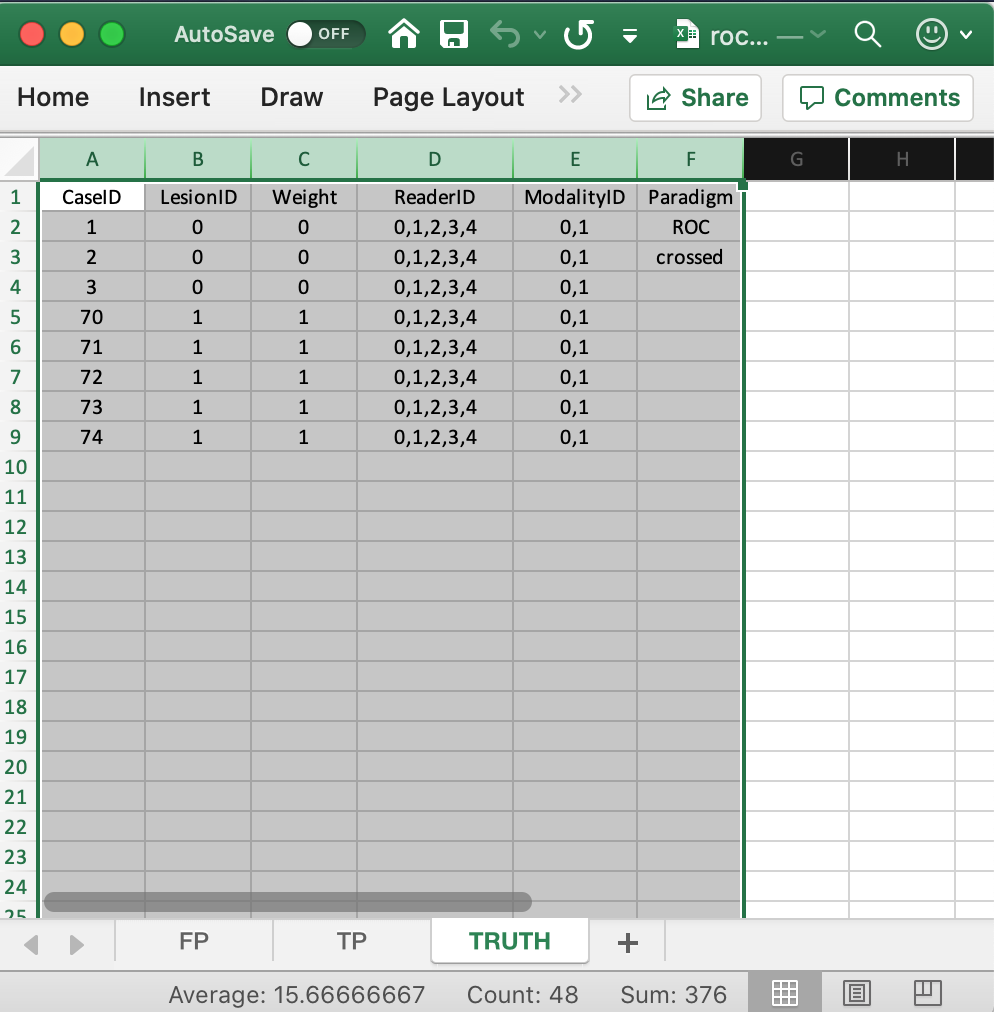
\includegraphics[width=0.5\linewidth,height=0.2\textheight]{images/rocCrTruth} 

}

\caption{Truth worksheet for file rocCr.xlsx}\label{fig:showRocCrTruthSheet}
\end{figure}

\hypertarget{the-structure-of-an-roc-dataset}{%
\section{The structure of an ROC dataset}\label{the-structure-of-an-roc-dataset}}

In the following code chunk the first statement retrieves the name of the data file, located in a hidden directory that one need not be concerned with. The second statement reads the file using the function \texttt{DfReadDataFile()} and saves it to object \texttt{x}. The third statement shows the structure of the dataset object \texttt{x}.

\begin{Shaded}
\begin{Highlighting}[]
\NormalTok{rocCr <-}\StringTok{ }\KeywordTok{system.file}\NormalTok{(}\StringTok{"extdata"}\NormalTok{, }\StringTok{"toyFiles/ROC/rocCr.xlsx"}\NormalTok{,}
                        \DataTypeTok{package =} \StringTok{"RJafroc"}\NormalTok{, }\DataTypeTok{mustWork =} \OtherTok{TRUE}\NormalTok{)}
\NormalTok{x <-}\StringTok{ }\KeywordTok{DfReadDataFile}\NormalTok{(rocCr, }\DataTypeTok{newExcelFileFormat =} \OtherTok{TRUE}\NormalTok{)}
\KeywordTok{str}\NormalTok{(x)}
\CommentTok{#> List of 12}
\CommentTok{#>  $ NL           : num [1:2, 1:5, 1:8, 1] 1 3 2 3 2 2 1 2 3 2 ...}
\CommentTok{#>  $ LL           : num [1:2, 1:5, 1:5, 1] 5 5 5 5 5 5 5 5 5 5 ...}
\CommentTok{#>  $ lesionVector : int [1:5] 1 1 1 1 1}
\CommentTok{#>  $ lesionID     : num [1:5, 1] 1 1 1 1 1}
\CommentTok{#>  $ lesionWeight : num [1:5, 1] 1 1 1 1 1}
\CommentTok{#>  $ dataType     : chr "ROC"}
\CommentTok{#>  $ modalityID   : Named chr [1:2] "0" "1"}
\CommentTok{#>   ..- attr(*, "names")= chr [1:2] "0" "1"}
\CommentTok{#>  $ readerID     : Named chr [1:5] "0" "1" "2" "3" ...}
\CommentTok{#>   ..- attr(*, "names")= chr [1:5] "0" "1" "2" "3" ...}
\CommentTok{#>  $ design       : chr "CROSSED"}
\CommentTok{#>  $ normalCases  : int [1:3] 1 2 3}
\CommentTok{#>  $ abnormalCases: int [1:5] 70 71 72 73 74}
\CommentTok{#>  $ truthTableStr: num [1:2, 1:5, 1:8, 1:2] 1 1 1 1 1 1 1 1 1 1 ...}
\end{Highlighting}
\end{Shaded}

\begin{itemize}
\tightlist
\item
  In the above code chunk flag \texttt{newExcelFileFormat} is set to \texttt{TRUE} as otherwise columns D - F in the \texttt{Truth} worksheet are ignored and the dataset is assumed to be crossed, with \texttt{dataType} automatically determined from the contents of the FP and TP worksheets.
\item
  Flag \texttt{newExcelFileFormat\ =\ FALSE} is for compatibility with older JAFROC format Excel files, which did not have these columns in the \texttt{Truth} worksheet. Its usage is deprecated.
\item
  The dataset object \texttt{x} is a \texttt{list} variable with 12 members.
\item
  The \texttt{x\$NL} member, with dimension {[}2, 5, 8, 1{]}, contains the ratings of normal cases. The extra values in the third dimension, filled with \texttt{NAs}, are needed for compatibility with FROC datasets, as unlike ROC, false positives are possible on diseased cases.
\item
  The \texttt{x\$LL}, with dimension {[}2, 5, 5, 1{]}, contains the ratings of abnormal cases.
\item
  The \texttt{x\$lesionVector} member is a vector with 5 ones representing the 5 diseased cases in the dataset.
\item
  The \texttt{x\$lesionID} member is an array with 5 ones.
\item
  The \texttt{x\$lesionWeight} member is an array with 5 ones.
\item
  The \texttt{lesionVector}, \texttt{lesionID} and \texttt{lesionWeight} members are not used for ROC datasets. They are there for compatibility with FROC datasets.
\item
  The \texttt{dataType} member indicates that this is an \texttt{ROC} dataset.
\item
  The \texttt{x\$modalityID} member is a vector with two elements \texttt{"0"} and \texttt{"1"}, naming the two modalities.
\item
  The \texttt{x\$readerID} member is a vector with five elements \texttt{"0"}, \texttt{"1"}, \texttt{"2"}, \texttt{"3"} and \texttt{"4"}, naming the five readers.
\item
  The \texttt{x\$design} member is CROSSED; specifies the dataset design, which is ``CROSSED''.
\item
  The \texttt{x\$normalCases} member lists the integer names of the normal cases, 1, 2, 3.
\item
  The \texttt{x\$abnormalCases} member lists the integer names of the abnormal cases, 70, 71, 72, 73, 74.
\item
  The \texttt{x\$truthTableStr} member quantifies the structure of the dataset, as explained in \textbf{Chapter 00 Vignette \#3-\#5}.
\end{itemize}

\hypertarget{the-false-positive-fp-ratings}{%
\section{The false positive (FP) ratings}\label{the-false-positive-fp-ratings}}

These are found in the \texttt{FP} or \texttt{NL} worksheet, see below.

\begin{figure}

{\centering 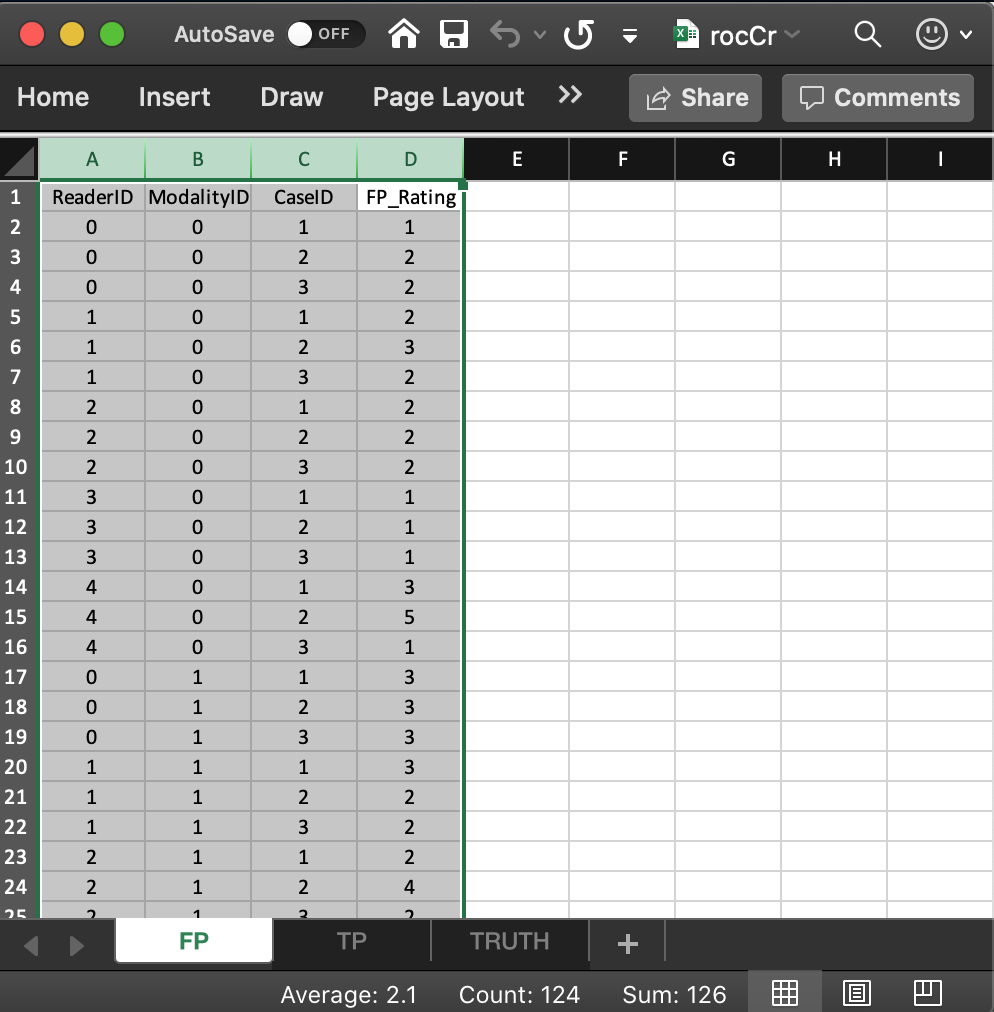
\includegraphics[width=0.5\linewidth,height=0.2\textheight]{images/rocCrFp} 

}

\caption{FP worksheet for file rocCr.xlsx}\label{fig:showRocCrFpSheet}
\end{figure}

\begin{itemize}
\tightlist
\item
  It consists of 4 columns, each of length 30 (= \# of modalities times number of readers times number of non-diseased cases).
\item
  \texttt{ReaderID}: the reader labels: \texttt{0}, \texttt{1}, \texttt{2}, \texttt{3} and \texttt{4}. Each reader label occurs 6 times (= \# of modalities times number of non-diseased cases).
\item
  \texttt{ModalityID}: the modality or treatment labels: \texttt{0} and \texttt{1}. Each label occurs 15 times (= \# of readers times number of non-diseased cases).
\item
  \texttt{CaseID}: the case labels for non-diseased cases: \texttt{1}, \texttt{2} and \texttt{3}. Each label occurs 10 times (= \# of modalities times \# of readers).
\item
  The label of a diseased case cannot occur in the FP worksheet. If it does the software generates an error.
\item
  \texttt{FP\_Rating}: the floating point ratings of non-diseased cases. Each row of this worksheet contains a rating corresponding to the values of \texttt{ReaderID}, \texttt{ModalityID} and \texttt{CaseID} for that row.
\end{itemize}

\hypertarget{the-true-positive-tp-ratings}{%
\section{The true positive (TP) ratings}\label{the-true-positive-tp-ratings}}

These are found in the \texttt{TP} or \texttt{LL} worksheet, see below.

\begin{figure}

{\centering 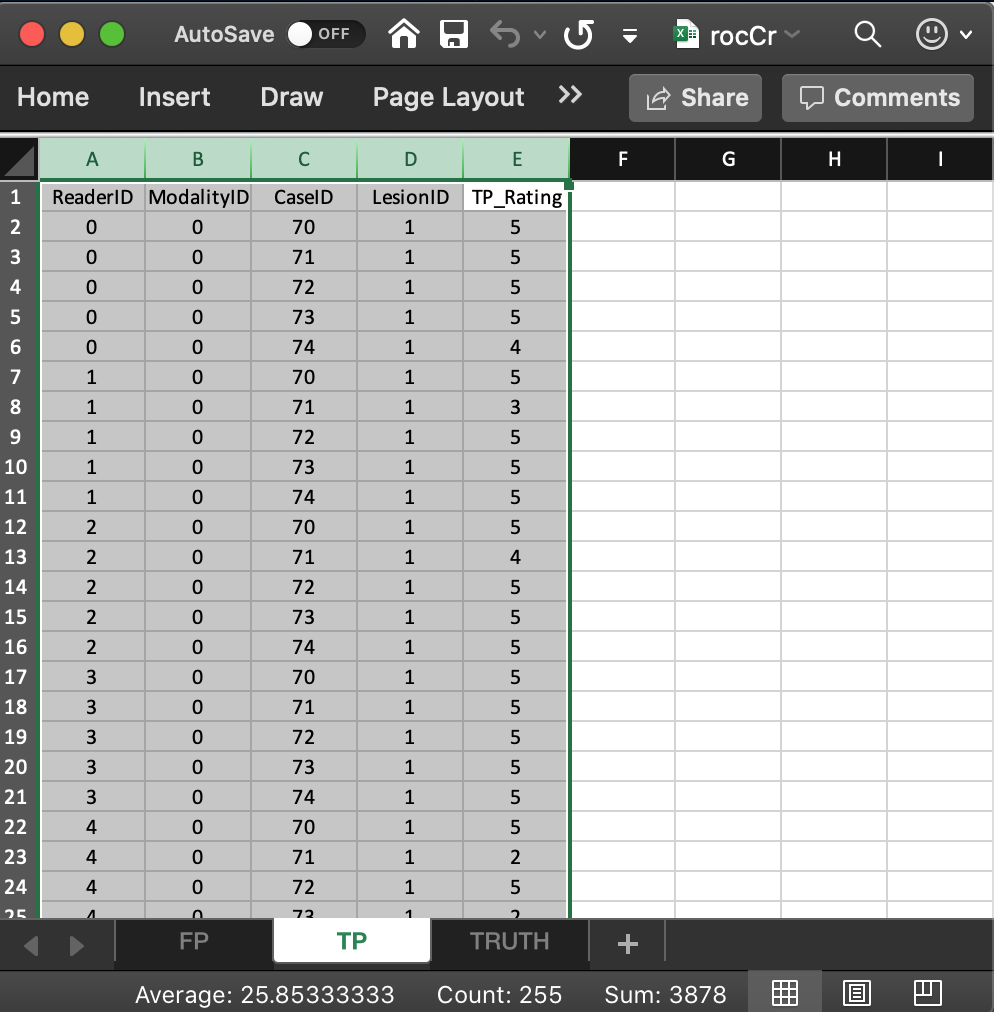
\includegraphics[width=0.5\linewidth,height=0.2\textheight]{images/rocCrTp} 

}

\caption{TP worksheet for file rocCr.xlsx}\label{fig:showRocCrTpSheet}
\end{figure}

\begin{itemize}
\tightlist
\item
  It consists of 5 columns, each of length 50 (= \# of modalities times number of readers times number of diseased cases).
\item
  \texttt{ReaderID}: the reader labels: \texttt{0}, \texttt{1}, \texttt{2}, \texttt{3} and \texttt{4}. Each reader label occurs 10 times (= \# of modalities times number of diseased cases).
\item
  \texttt{ModalityID}: the modality or treatment labels: \texttt{0} and \texttt{1}. Each label occurs 25 times (= \# of readers times number of diseased cases).
\item
  \texttt{LesionID}: For an ROC dataset this column contains fifty 1's (each diseased case has one lesion).
\item
  \texttt{CaseID}: the case labels for non-diseased cases: \texttt{70}, \texttt{71}, \texttt{72}, \texttt{73} and \texttt{74}. Each label occurs 10 times (= \# of modalities times \# of readers). The label of a non-diseased case cannot occur in the TP worksheet.
\item
  \texttt{TP\_Rating}: the floating point ratings of diseased cases. Each row of this worksheet contains a rating corresponding to the values of \texttt{ReaderID}, \texttt{ModalityID}, \texttt{LesionID} and \texttt{CaseID} for that row.
\end{itemize}

\hypertarget{correspondence-between-nl-member-of-dataset-and-the-fp-worksheet}{%
\section{\texorpdfstring{Correspondence between \texttt{NL} member of dataset and the \texttt{FP} worksheet}{Correspondence between NL member of dataset and the FP worksheet}}\label{correspondence-between-nl-member-of-dataset-and-the-fp-worksheet}}

\begin{itemize}
\tightlist
\item
  The list member \texttt{x\$NL} is an array with \texttt{dim\ =\ c(2,5,8,1)}.

  \begin{itemize}
  \tightlist
  \item
    The first dimension (2) comes from the number of modalities.
  \item
    The second dimension (5) comes from the number of readers.
  \item
    The third dimension (8) comes from the \textbf{total} number of cases.
  \item
    The fourth dimension is alway 1 for an ROC dataset.
  \end{itemize}
\item
  The value of \texttt{x\$NL{[}1,5,2,1{]}}, i.e., 5, corresponds to row 15 of the FP table, i.e., to \texttt{ModalityID} = 0, \texttt{ReaderID} = 4 and \texttt{CaseID} = 2.
\item
  The value of \texttt{x\$NL{[}2,3,2,1{]}}, i.e., 4, corresponds to row 24 of the FP table, i.e., to \texttt{ModalityID} 1, \texttt{ReaderID} 2 and \texttt{CaseID} 2.
\item
  All values for case index \textgreater{} 3 are \texttt{-Inf}. For example the value of \texttt{x\$NL{[}2,3,4,1{]}} is \texttt{-Inf}. This is because there are only 3 non-diseased cases. The extra length is needed for compatibility with FROC datasets.
\end{itemize}

\hypertarget{correspondence-between-ll-member-of-dataset-and-the-tp-worksheet}{%
\section{\texorpdfstring{Correspondence between \texttt{LL} member of dataset and the \texttt{TP} worksheet}{Correspondence between LL member of dataset and the TP worksheet}}\label{correspondence-between-ll-member-of-dataset-and-the-tp-worksheet}}

\begin{itemize}
\tightlist
\item
  The list member \texttt{x\$LL} is an array with \texttt{dim\ =\ c(2,5,5,1)}.

  \begin{itemize}
  \tightlist
  \item
    The first dimension (2) comes from the number of modalities.
  \item
    The second dimension (5) comes from the number of readers.
  \item
    The third dimension (5) comes from the number of diseased cases.
  \item
    The fourth dimension is alway 1 for an ROC dataset.
  \end{itemize}
\item
  The value of \texttt{x\$LL{[}1,1,5,1{]}}, i.e., 4, corresponds to row 6 of the TP table, i.e., to \texttt{ModalityID} = 0, \texttt{ReaderID} = 0 and \texttt{CaseID} = 74.
\item
  The value of \texttt{x\$LL{[}1,2,2,1{]}}, i.e., 3, corresponds to row 8 of the TP table, i.e., to \texttt{ModalityID} = 0, \texttt{ReaderID} = 1 and \texttt{CaseID} = 71.
\item
  There are no -Inf values in \texttt{x\$LL}: \texttt{any(x\$LL\ ==\ -Inf)} = FALSE.
\end{itemize}

\hypertarget{correspondence-using-the-which-function}{%
\section{\texorpdfstring{Correspondence using the \texttt{which} function}{Correspondence using the which function}}\label{correspondence-using-the-which-function}}

\begin{itemize}
\tightlist
\item
  Converting from \textbf{names} to \textbf{subscripts} (indicating position in an array) can be confusing.
\item
  The following example uses the \texttt{which} function to help out.
\item
  The first line says that the \texttt{abnormalCase} named 70 corresponds to subscript 1 in the LL array case dimension.
\item
  The second line prints the NL rating for \texttt{modalityID} = 0, \texttt{readerID} = 1 and \texttt{normalCases} = 1.
\item
  The third line prints the LL rating for \texttt{modalityID} = 0, \texttt{readerID} = 1 and \texttt{abnormalCases} = 70.
\item
  The last line shows what happens if one enters an invalid value for name; the result is a \texttt{numeric(0)}.
\item
  Note that in each of these examples, the last dimension is 1 because we are dealing with an ROC dataset.
\item
  The reader is encouraged to examine the correspondence between the NL and LL ratings and the Excel file using this method.
\end{itemize}

\begin{Shaded}
\begin{Highlighting}[]
\KeywordTok{which}\NormalTok{(x}\OperatorTok{$}\NormalTok{abnormalCases }\OperatorTok{==}\StringTok{ }\DecValTok{70}\NormalTok{)}
\CommentTok{#> [1] 1}
\NormalTok{x}\OperatorTok{$}\NormalTok{NL[}\KeywordTok{which}\NormalTok{(x}\OperatorTok{$}\NormalTok{modalityID }\OperatorTok{==}\StringTok{ "0"}\NormalTok{),}\KeywordTok{which}\NormalTok{(x}\OperatorTok{$}\NormalTok{readerID }\OperatorTok{==}\StringTok{ "1"}\NormalTok{),}\KeywordTok{which}\NormalTok{(x}\OperatorTok{$}\NormalTok{normalCases }\OperatorTok{==}\StringTok{ }\DecValTok{1}\NormalTok{),}\DecValTok{1}\NormalTok{]}
\CommentTok{#> [1] 2}
\NormalTok{x}\OperatorTok{$}\NormalTok{LL[}\KeywordTok{which}\NormalTok{(x}\OperatorTok{$}\NormalTok{modalityID }\OperatorTok{==}\StringTok{ "0"}\NormalTok{),}\KeywordTok{which}\NormalTok{(x}\OperatorTok{$}\NormalTok{readerID }\OperatorTok{==}\StringTok{ "1"}\NormalTok{),}\KeywordTok{which}\NormalTok{(x}\OperatorTok{$}\NormalTok{abnormalCases }\OperatorTok{==}\StringTok{ }\DecValTok{70}\NormalTok{),}\DecValTok{1}\NormalTok{]}
\CommentTok{#> [1] 5}
\NormalTok{x}\OperatorTok{$}\NormalTok{LL[}\KeywordTok{which}\NormalTok{(x}\OperatorTok{$}\NormalTok{modalityID }\OperatorTok{==}\StringTok{ "a"}\NormalTok{),}\KeywordTok{which}\NormalTok{(x}\OperatorTok{$}\NormalTok{readerID }\OperatorTok{==}\StringTok{ "1"}\NormalTok{),}\KeywordTok{which}\NormalTok{(x}\OperatorTok{$}\NormalTok{abnormalCases }\OperatorTok{==}\StringTok{ }\DecValTok{70}\NormalTok{),}\DecValTok{1}\NormalTok{]}
\CommentTok{#> numeric(0)}
\end{Highlighting}
\end{Shaded}

\hypertarget{references-1}{%
\section{References}\label{references-1}}

\hypertarget{frocdataformat}{%
\chapter{FROC data format}\label{frocdataformat}}

\hypertarget{purpose}{%
\section{Purpose}\label{purpose}}

\begin{itemize}
\tightlist
\item
  Explain the data format of the input Excel file for FROC datasets.
\item
  Explain the format of the FROC dataset.
\item
  Explain the lesion distribution array returned by \texttt{UtilLesionDistr()}.
\item
  Explain the lesion weights array returned by \texttt{UtilLesionWeightsDistr()}.
\item
  Details on the FROC paradigm are in my book.
\end{itemize}

\hypertarget{introduction-1}{%
\section{Introduction}\label{introduction-1}}

\begin{itemize}
\tightlist
\item
  See my book \citet{RN2680} for full details.
\item
  In the Free-response Receiver Operating Characteristic (FROC) paradigm \citep{RN761} the observer searches each case for signs of \textbf{localized disease} and marks and rates localized regions that are sufficiently suspicious for disease presence.
\item
  FROC data consists of \textbf{mark-rating pairs}, where each mark is a localized-region that was considered sufficiently suspicious for presence of a localized lesion and the rating is the corresponding confidence level.
\item
  By adopting a proximity criterion, each mark is classified by the investigator as a lesion localization (\texttt{LL}) - if it is close to a real lesion - or a non-lesion localization (\texttt{NL}) otherwise.
\item
  The observer assigns a rating to each region. The rating, as in the ROC paradigm, can be an integer or quasi-continuous (e.g., 0 -- 100), or a floating point value, as long as higher numbers represent greater confidence in presence of a lesion at the indicated region.
\end{itemize}

\hypertarget{the-excel-data-format-1}{%
\section{The Excel data format}\label{the-excel-data-format-1}}

The Excel file has three worsheets. These are named \texttt{Truth}, \texttt{NL} or \texttt{FP} and \texttt{LL} or \texttt{TP}.

\hypertarget{the-truth-worksheet-1}{%
\section{\texorpdfstring{The \texttt{Truth} worksheet}{The Truth worksheet}}\label{the-truth-worksheet-1}}

The \texttt{Truth} worksheet contains 6 columns: \texttt{CaseID}, \texttt{LesionID}, \texttt{Weight}, \texttt{ReaderID}, \texttt{ModalityID} and \texttt{Paradigm}.

\begin{itemize}
\tightlist
\item
  Since a diseased case may have more than one lesion, the first five columns contain \textbf{at least} as many rows as there are cases (images) in the dataset.
\item
  \texttt{CaseID}: unique \textbf{integers}, one per case, representing the cases in the dataset.
\item
  \texttt{LesionID}: integers 0, 1, 2, etc., with each 0 representing a non-diseased case, 1 representing the \emph{first} lesion on a diseased case, 2 representing the second lesion on a diseased case, if present, and so on.
\item
  The non-diseased cases are labeled \texttt{1}, \texttt{2} and \texttt{3}, while the diseased cases are labeled \texttt{70}, \texttt{71}, \texttt{72}, \texttt{73} and \texttt{74}.
\item
  There are 3 non-diseased cases in the dataset (the number of 0's in the \texttt{LesionID} column).
\item
  There are 5 diseased cases in the dataset (the number of 1's in the \texttt{LesionID} column of the \texttt{Truth} worksheet).
\item
  There are 3 readers in the dataset (each cell in the \texttt{ReaderID} column contains \texttt{0,\ 1,\ 2}).
\item
  There are 2 modalities in the dataset (each cell in the \texttt{ModalityID} column contains \texttt{0,\ 1}).
\item
  \texttt{Weight}: floating point; 0, for each non-diseased case, or values for each diseased case that add up to unity.\\
\item
  Diseased case \texttt{70} has two lesions, with \texttt{LesionID}s 1 and 2, and weights 0.3 and 0.7. Diseased case \texttt{71} has one lesion, with \texttt{LesionID} = 1, and \texttt{Weight} = 1. Diseased case \texttt{72} has three lesions, with \texttt{LesionID}s 1, 2 and 3 and weights 1/3 each. Diseased case \texttt{73} has two lesions, with \texttt{LesionID}s 1, and 2 and weights 0.1 and 0.9. Diseased case \texttt{74} has one lesion, with \texttt{LesionID} = 1 and \texttt{Weight} = 1.
\item
  \texttt{ReaderID}: a comma-separated listing of readers, each represented by a unique \textbf{integer}, that have interpreted the case. In the example shown below each cell has the value \texttt{0,\ 1,\ 2}. \textbf{Each cell has to be text formatted. Otherwise Excel will not accept it.}
\item
  \texttt{ModalityID}: a comma-separated listing of modalities (or treatments), each represented by a unique \textbf{integer}, that apply to each case. In the example each cell has the value \texttt{0,\ 1}. \textbf{Each cell has to be text formatted.}
\item
  \texttt{Paradigm}: In the example shown below, the contents are \texttt{FROC} and \texttt{crossed}. It informs the software that this is an \texttt{FROC} dataset and the design is ``crossed'', as in \textbf{Vignette \#1}.
\end{itemize}

\begin{figure}

{\centering 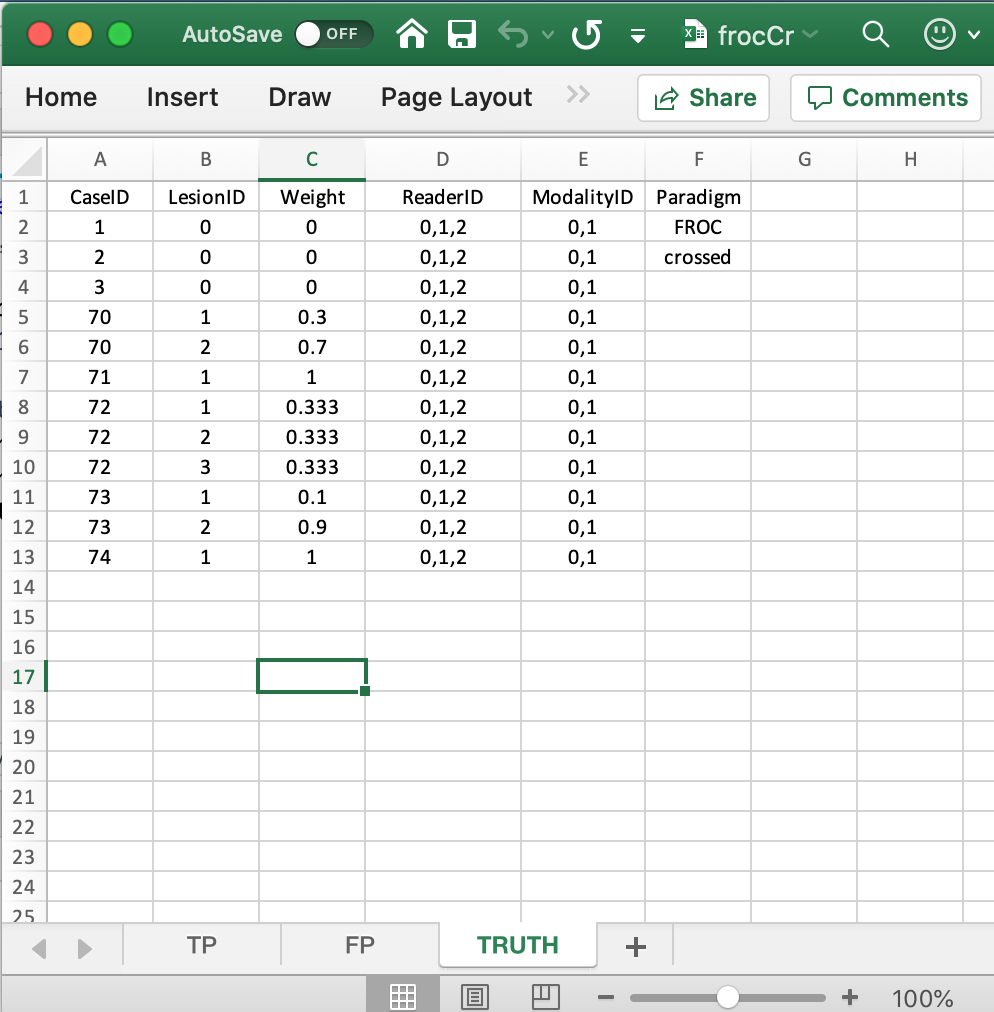
\includegraphics[width=0.5\linewidth,height=0.2\textheight]{images/frocCrTruth} 

}

\caption{Truth worksheet for file inst/extdata/toyFiles/FROC/frocCr.xlsx}\label{fig:frocCrTruth}
\end{figure}

\hypertarget{the-structure-of-an-froc-dataset}{%
\section{The structure of an FROC dataset}\label{the-structure-of-an-froc-dataset}}

The example shown above corresponds to Excel file \texttt{inst/extdata/toyFiles/FROC/frocCr.xlsx} in the project directory.

\begin{Shaded}
\begin{Highlighting}[]
\NormalTok{frocCr <-}\StringTok{ }\KeywordTok{system.file}\NormalTok{(}\StringTok{"extdata"}\NormalTok{, }\StringTok{"toyFiles/FROC/frocCr.xlsx"}\NormalTok{,}
                        \DataTypeTok{package =} \StringTok{"RJafroc"}\NormalTok{, }\DataTypeTok{mustWork =} \OtherTok{TRUE}\NormalTok{)}
\NormalTok{x <-}\StringTok{ }\KeywordTok{DfReadDataFile}\NormalTok{(frocCr, }\DataTypeTok{newExcelFileFormat =} \OtherTok{TRUE}\NormalTok{)}
\KeywordTok{str}\NormalTok{(x)}
\CommentTok{#> List of 12}
\CommentTok{#>  $ NL           : num [1:2, 1:3, 1:8, 1:2] 1.02 2.89 2.21 3.01 2.14 ...}
\CommentTok{#>  $ LL           : num [1:2, 1:3, 1:5, 1:3] 5.28 5.2 5.14 4.77 4.66 4.87 3.01 3.27 3.31 3.19 ...}
\CommentTok{#>  $ lesionVector : int [1:5] 2 1 3 2 1}
\CommentTok{#>  $ lesionID     : num [1:5, 1:3] 1 1 1 1 1 ...}
\CommentTok{#>  $ lesionWeight : num [1:5, 1:3] 0.3 1 0.333 0.1 1 ...}
\CommentTok{#>  $ dataType     : chr "FROC"}
\CommentTok{#>  $ modalityID   : Named chr [1:2] "0" "1"}
\CommentTok{#>   ..- attr(*, "names")= chr [1:2] "0" "1"}
\CommentTok{#>  $ readerID     : Named chr [1:3] "0" "1" "2"}
\CommentTok{#>   ..- attr(*, "names")= chr [1:3] "0" "1" "2"}
\CommentTok{#>  $ design       : chr "CROSSED"}
\CommentTok{#>  $ normalCases  : int [1:3] 1 2 3}
\CommentTok{#>  $ abnormalCases: int [1:5] 70 71 72 73 74}
\CommentTok{#>  $ truthTableStr: num [1:2, 1:3, 1:8, 1:4] 1 1 1 1 1 1 1 1 1 1 ...}
\end{Highlighting}
\end{Shaded}

\begin{itemize}
\tightlist
\item
  This follows the general description in \textbf{Vignette \#1}. The differences are described below.
\item
  The \texttt{x\$dataType} member indicates that this is an \texttt{FROC} dataset.
\item
  The \texttt{x\$lesionVector} member is a vector whose contents reflect the number of lesions in each diseased case, i.e., 2, 1, 3, 2, 1 in the current example.
\item
  The \texttt{x\$lesionID} member indicates the labeling of the lesions in each diseased case.
\end{itemize}

\begin{Shaded}
\begin{Highlighting}[]
\NormalTok{x}\OperatorTok{$}\NormalTok{lesionID}
\CommentTok{#>      [,1] [,2] [,3]}
\CommentTok{#> [1,]    1    2 -Inf}
\CommentTok{#> [2,]    1 -Inf -Inf}
\CommentTok{#> [3,]    1    2    3}
\CommentTok{#> [4,]    1    2 -Inf}
\CommentTok{#> [5,]    1 -Inf -Inf}
\end{Highlighting}
\end{Shaded}

\begin{itemize}
\tightlist
\item
  This shows that the lesions on the first diseased case are labeled 1 and 2. The \texttt{-Inf} is a filler used to denote a missing value. The second diseased case has one lesion labeled 1. The third diseased case has three lesions labeled 1, 2 and 3, etc.
\item
  The \texttt{lesionWeight} member is the clinical importance of each lesion. Lacking specific clinical reasons, the lesions should be equally weighted; this is \emph{not} true for this toy dataset.
\end{itemize}

\begin{Shaded}
\begin{Highlighting}[]
\NormalTok{x}\OperatorTok{$}\NormalTok{lesionWeight}
\CommentTok{#>           [,1]      [,2]      [,3]}
\CommentTok{#> [1,] 0.3000000 0.7000000      -Inf}
\CommentTok{#> [2,] 1.0000000      -Inf      -Inf}
\CommentTok{#> [3,] 0.3333333 0.3333333 0.3333333}
\CommentTok{#> [4,] 0.1000000 0.9000000      -Inf}
\CommentTok{#> [5,] 1.0000000      -Inf      -Inf}
\end{Highlighting}
\end{Shaded}

\begin{itemize}
\tightlist
\item
  The first diseased case has two lesions, the first has weight 0.3 and the second has weight 0.7. The second diseased case has one lesion with weight 1.The third diseased case has three equally weighted lesions, each with weight 1/3. Etc.
\end{itemize}

\hypertarget{the-false-positive-fp-ratings-1}{%
\section{The false positive (FP) ratings}\label{the-false-positive-fp-ratings-1}}

These are found in the \texttt{FP} or \texttt{NL} worksheet, see below.

\begin{figure}

{\centering 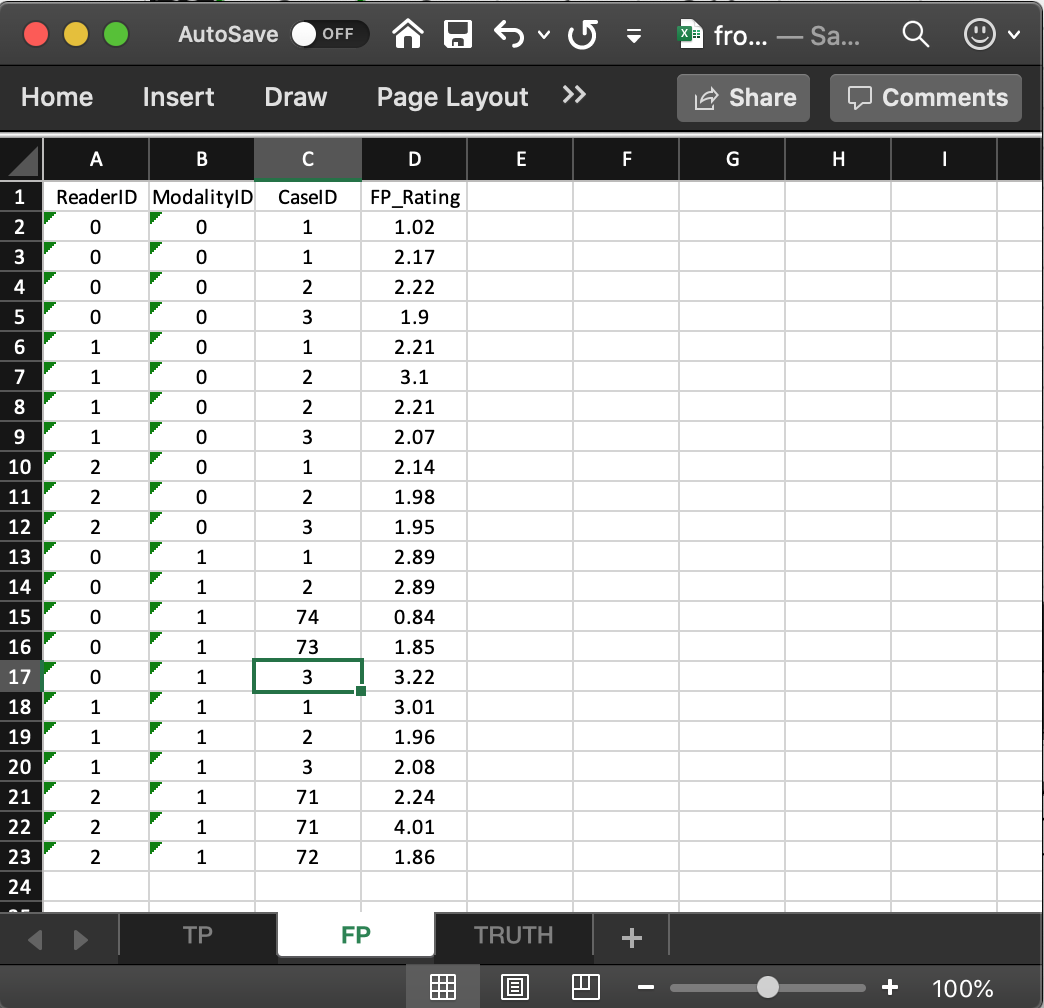
\includegraphics[width=0.5\linewidth,height=0.2\textheight]{images/frocCrNL} 

}

\caption{Fig. 2: FP/NL worksheet for file inst/extdata/toyFiles/FROC/frocCr.xlsx}\label{fig:frocCrNL}
\end{figure}

\begin{itemize}
\tightlist
\item
  It consists of 4 columns, of equal length. \textbf{The common length is unpredictable.} It could be zero if the dataset has no NL marks (a distinct possibility if the lesions are very easy to find and the modality and/or observer has high performance). All one knows is that the common length is an integer greater than or equal to zero.
\item
  In the example dataset, the common length is 22.
\item
  \texttt{ReaderID}: the reader labels: these must be \texttt{0}, \texttt{1}, or \texttt{2}, as declared in the \texttt{Truth} worksheet.
\item
  \texttt{ModalityID}: the modality labels: must be \texttt{0} or \texttt{1}, as declared in the \texttt{Truth} worksheet.
\item
  \texttt{CaseID}: the labels of cases with \texttt{NL} marks. In the FROC paradigm, \texttt{NL} events can occur on non-diseased \textbf{and} diseased cases.
\item
  \texttt{FP\_Rating}: the floating point ratings of \texttt{NL} marks. Each row of this worksheet yields a rating corresponding to the values of \texttt{ReaderID}, \texttt{ModalityID} and \texttt{CaseID} for that row.
\item
  For \texttt{ModalityID} 0, \texttt{ReaderID} 0 and \texttt{CaseID} 1 (the first non-diseased case declared in the \texttt{Truth} worksheet), there is a single \texttt{NL} mark that was rated 1.02, corresponding to row 2 of the \texttt{FP} worksheet.
\item
  Diseased cases with \texttt{NL} marks are also declared in the \texttt{FP} worksheet. Some examples are seen at rows 15, 16 and 21-23 of the \texttt{FP} worksheet.
\item
  Rows 21 and 22 show that \texttt{caseID} = 71 got two \texttt{NL} marks, rated 2.24, 4.01.
\item
  That this is the \emph{only} case with two marks determines the length of the fourth dimension of the \texttt{x\$NL} list member, 2 in the current example. Absent this case, the length would have been one.
\item
  In general, the case with the most \texttt{NL} marks determines the length of the fourth dimension of the \texttt{x\$NL} list member.
\item
  The reader should convince oneself that the ratings in \texttt{x\$NL} reflect the contents of the \texttt{FP} worksheet.
\end{itemize}

\hypertarget{the-true-positive-tp-ratings-1}{%
\section{The true positive (TP) ratings}\label{the-true-positive-tp-ratings-1}}

These are found in the \texttt{TP} or \texttt{LL} worksheet, see below.

\begin{figure}

{\centering 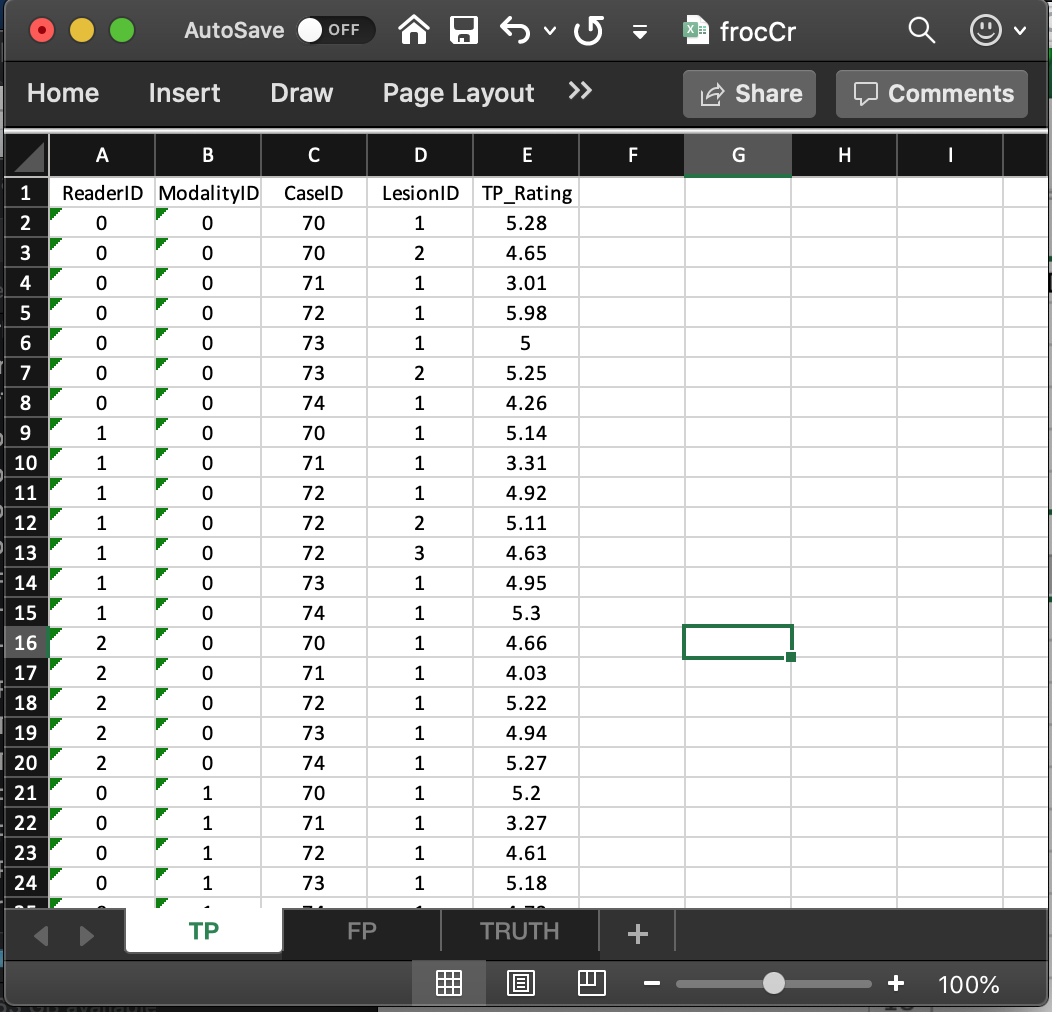
\includegraphics[width=0.5\linewidth,height=0.2\textheight]{images/frocCrLL} 

}

\caption{Fig. 3: TP/LL worksheet for file inst/extdata/toyFiles/FROC/frocCr.xlsx}\label{fig:frocCrLL}
\end{figure}

\begin{itemize}
\tightlist
\item
  This worksheet can only have diseased cases. The presence of a non-diseased case in this worksheet will generate an error.
\item
  The common vertical length, 31 in this example, is a-priori unpredictable. Given the structure of the \texttt{Truth} worsheet for this dataset, the maximum length would be 9 times 2 times 3, assuming every lesion is marked for each modality, reader and diseased case. The 9 comes from the total number of non-zero entries in the \texttt{LesionID} column of the \texttt{Truth} worksheet.
\item
  The fact that the length is smaller than the maximum length means that there are combinations of modality, reader and diseased cases on which some lesions were not marked.
\item
  As an example, the first lesion in \texttt{CaseID} equal to \texttt{70} was marked (and rated 5.28) in \texttt{ModalityID} \texttt{0} and \texttt{ReaderID} \texttt{0}.
\item
  The length of the fourth dimension of the \texttt{x\$LL} list member, 3 in the present example, is determined by the diseased case with the most lesions in the \texttt{Truth} worksheet.
\item
  The reader should convince oneself that the ratings in \texttt{x\$LL} reflect the contents of the \texttt{TP} worksheet.
\end{itemize}

\hypertarget{on-the-distribution-of-numbers-of-lesions-in-abnormal-cases}{%
\section{On the distribution of numbers of lesions in abnormal cases}\label{on-the-distribution-of-numbers-of-lesions-in-abnormal-cases}}

\begin{itemize}
\tightlist
\item
  Consider a much larger dataset, \texttt{dataset11}, with structure as shown below:
\end{itemize}

\begin{Shaded}
\begin{Highlighting}[]
\NormalTok{x <-}\StringTok{ }\NormalTok{dataset11}
\KeywordTok{str}\NormalTok{(x)}
\CommentTok{#> List of 12}
\CommentTok{#>  $ NL           : num [1:4, 1:5, 1:158, 1:4] -Inf -Inf -Inf -Inf -Inf ...}
\CommentTok{#>  $ LL           : num [1:4, 1:5, 1:115, 1:20] -Inf -Inf -Inf -Inf -Inf ...}
\CommentTok{#>  $ lesionVector : int [1:115] 6 4 7 1 3 3 3 8 11 2 ...}
\CommentTok{#>  $ lesionID     : num [1:115, 1:20] 1 1 1 1 1 1 1 1 1 1 ...}
\CommentTok{#>  $ lesionWeight : num [1:115, 1:20] 0.167 0.25 0.143 1 0.333 ...}
\CommentTok{#>  $ dataType     : chr "FROC"}
\CommentTok{#>  $ modalityID   : Named chr [1:4] "1" "2" "3" "4"}
\CommentTok{#>   ..- attr(*, "names")= chr [1:4] "1" "2" "3" "4"}
\CommentTok{#>  $ readerID     : Named chr [1:5] "1" "2" "3" "4" ...}
\CommentTok{#>   ..- attr(*, "names")= chr [1:5] "1" "2" "3" "4" ...}
\CommentTok{#>  $ design       : chr "CROSSED"}
\CommentTok{#>  $ normalCases  : int [1:43] 6 9 14 27 62 66 70 71 83 91 ...}
\CommentTok{#>  $ abnormalCases: int [1:115] 1 2 3 5 7 8 10 11 13 17 ...}
\CommentTok{#>  $ truthTableStr: num [1:4, 1:5, 1:158, 1:21] 1 1 1 1 1 1 1 1 1 1 ...}
\end{Highlighting}
\end{Shaded}

\begin{itemize}
\tightlist
\item
  Focus for now in the 115 abnormal cases.
\item
  The numbers of lesions in these cases is contained in \texttt{x\$lesionVector}.
\end{itemize}

\begin{Shaded}
\begin{Highlighting}[]
\NormalTok{x}\OperatorTok{$}\NormalTok{lesionVector}
\CommentTok{#>   [1]  6  4  7  1  3  3  3  8 11  2  4  6  2 16  5  2  8  3  4  7 11  1  4  3  4}
\CommentTok{#>  [26]  4  7  3  2  5  2  2  7  6  6  4 10 20 12  6  4  7 12  5  1  1  5  1  2  8}
\CommentTok{#>  [51]  3  1  2  2  3  2  8 16 10  1  2  2  6  3  2  2  4  6 10 11  1  2  6  2  4}
\CommentTok{#>  [76]  5  2  9  6  6  8  3  8  7  1  1  6  3  2  1  9  8  8  2  2 12  1  1  1  1}
\CommentTok{#> [101]  1  3  1  2  2  1  1  1  1  3  1  1  1  2  1}
\end{Highlighting}
\end{Shaded}

\begin{itemize}
\tightlist
\item
  For example, the first abnormal case contains 6 lesions, the second contains 4 lesions, the third contains 7 lesions, etc. and the last abnormal case contains 1 lesion.
\item
  To get an idea of the distribution of the numbers of lesions per abnormal cases, one could interrogate this vector as shown below using the \texttt{which()} function:
\end{itemize}

\begin{Shaded}
\begin{Highlighting}[]
\ControlFlowTok{for}\NormalTok{ (el }\ControlFlowTok{in} \DecValTok{1}\OperatorTok{:}\KeywordTok{max}\NormalTok{(x}\OperatorTok{$}\NormalTok{lesionVector)) }\KeywordTok{cat}\NormalTok{(}
  \StringTok{"abnormal cases with"}\NormalTok{, el, }\StringTok{"lesions = "}\NormalTok{, }
  \KeywordTok{length}\NormalTok{(}\KeywordTok{which}\NormalTok{(x}\OperatorTok{$}\NormalTok{lesionVector }\OperatorTok{==}\StringTok{ }\NormalTok{el)), }\StringTok{"}\CharTok{\textbackslash{}n}\StringTok{"}\NormalTok{)}
\CommentTok{#> abnormal cases with 1 lesions =  25 }
\CommentTok{#> abnormal cases with 2 lesions =  23 }
\CommentTok{#> abnormal cases with 3 lesions =  13 }
\CommentTok{#> abnormal cases with 4 lesions =  10 }
\CommentTok{#> abnormal cases with 5 lesions =  5 }
\CommentTok{#> abnormal cases with 6 lesions =  11 }
\CommentTok{#> abnormal cases with 7 lesions =  6 }
\CommentTok{#> abnormal cases with 8 lesions =  8 }
\CommentTok{#> abnormal cases with 9 lesions =  2 }
\CommentTok{#> abnormal cases with 10 lesions =  3 }
\CommentTok{#> abnormal cases with 11 lesions =  3 }
\CommentTok{#> abnormal cases with 12 lesions =  3 }
\CommentTok{#> abnormal cases with 13 lesions =  0 }
\CommentTok{#> abnormal cases with 14 lesions =  0 }
\CommentTok{#> abnormal cases with 15 lesions =  0 }
\CommentTok{#> abnormal cases with 16 lesions =  2 }
\CommentTok{#> abnormal cases with 17 lesions =  0 }
\CommentTok{#> abnormal cases with 18 lesions =  0 }
\CommentTok{#> abnormal cases with 19 lesions =  0 }
\CommentTok{#> abnormal cases with 20 lesions =  1}
\end{Highlighting}
\end{Shaded}

\begin{itemize}
\tightlist
\item
  This tells us that 25 cases contain 1 lesion
\item
  Likewise, 23 cases contain 2 lesions
\item
  Etc.
\end{itemize}

\hypertarget{definition-of-lesdistr-array}{%
\subsection{\texorpdfstring{Definition of \texttt{lesDistr} array}{Definition of lesDistr array}}\label{definition-of-lesdistr-array}}

\begin{itemize}
\tightlist
\item
  Let us ask what is the fraction of (abnormal) cases with 1 lesion, 2 lesions etc.
\end{itemize}

\begin{Shaded}
\begin{Highlighting}[]
\ControlFlowTok{for}\NormalTok{ (el }\ControlFlowTok{in} \DecValTok{1}\OperatorTok{:}\KeywordTok{max}\NormalTok{(x}\OperatorTok{$}\NormalTok{lesionVector)) }\KeywordTok{cat}\NormalTok{(}\StringTok{"fraction of abnormal cases with"}\NormalTok{, el, }\StringTok{"lesions = "}\NormalTok{, }
                                              \KeywordTok{length}\NormalTok{(}\KeywordTok{which}\NormalTok{(x}\OperatorTok{$}\NormalTok{lesionVector }\OperatorTok{==}\StringTok{ }\NormalTok{el))}\OperatorTok{/}\KeywordTok{length}\NormalTok{(x}\OperatorTok{$}\NormalTok{LL[}\DecValTok{1}\NormalTok{,}\DecValTok{1}\NormalTok{,,}\DecValTok{1}\NormalTok{]), }\StringTok{"}\CharTok{\textbackslash{}n}\StringTok{"}\NormalTok{)}
\CommentTok{#> fraction of abnormal cases with 1 lesions =  0.2173913 }
\CommentTok{#> fraction of abnormal cases with 2 lesions =  0.2 }
\CommentTok{#> fraction of abnormal cases with 3 lesions =  0.1130435 }
\CommentTok{#> fraction of abnormal cases with 4 lesions =  0.08695652 }
\CommentTok{#> fraction of abnormal cases with 5 lesions =  0.04347826 }
\CommentTok{#> fraction of abnormal cases with 6 lesions =  0.09565217 }
\CommentTok{#> fraction of abnormal cases with 7 lesions =  0.05217391 }
\CommentTok{#> fraction of abnormal cases with 8 lesions =  0.06956522 }
\CommentTok{#> fraction of abnormal cases with 9 lesions =  0.0173913 }
\CommentTok{#> fraction of abnormal cases with 10 lesions =  0.02608696 }
\CommentTok{#> fraction of abnormal cases with 11 lesions =  0.02608696 }
\CommentTok{#> fraction of abnormal cases with 12 lesions =  0.02608696 }
\CommentTok{#> fraction of abnormal cases with 13 lesions =  0 }
\CommentTok{#> fraction of abnormal cases with 14 lesions =  0 }
\CommentTok{#> fraction of abnormal cases with 15 lesions =  0 }
\CommentTok{#> fraction of abnormal cases with 16 lesions =  0.0173913 }
\CommentTok{#> fraction of abnormal cases with 17 lesions =  0 }
\CommentTok{#> fraction of abnormal cases with 18 lesions =  0 }
\CommentTok{#> fraction of abnormal cases with 19 lesions =  0 }
\CommentTok{#> fraction of abnormal cases with 20 lesions =  0.008695652}
\end{Highlighting}
\end{Shaded}

\begin{itemize}
\tightlist
\item
  This tells us that fraction 0.217 of (abnormal) cases contain 1 lesion
\item
  And fraction 0.2 of (abnormal) cases contain 2 lesions
\item
  Etc.
\item
  This information is contained the the \texttt{lesDistr} array
\item
  It is coded in the \texttt{Utility} function \texttt{UtilLesionDistr()}
\end{itemize}

\begin{Shaded}
\begin{Highlighting}[]
\NormalTok{lesDistr <-}\StringTok{ }\KeywordTok{UtilLesionDistr}\NormalTok{(x)}
\NormalTok{lesDistr}
\CommentTok{#>       [,1]        [,2]}
\CommentTok{#>  [1,]    1 0.217391304}
\CommentTok{#>  [2,]    2 0.200000000}
\CommentTok{#>  [3,]    3 0.113043478}
\CommentTok{#>  [4,]    4 0.086956522}
\CommentTok{#>  [5,]    5 0.043478261}
\CommentTok{#>  [6,]    6 0.095652174}
\CommentTok{#>  [7,]    7 0.052173913}
\CommentTok{#>  [8,]    8 0.069565217}
\CommentTok{#>  [9,]    9 0.017391304}
\CommentTok{#> [10,]   10 0.026086957}
\CommentTok{#> [11,]   11 0.026086957}
\CommentTok{#> [12,]   12 0.026086957}
\CommentTok{#> [13,]   16 0.017391304}
\CommentTok{#> [14,]   20 0.008695652}
\end{Highlighting}
\end{Shaded}

\begin{itemize}
\tightlist
\item
  The \texttt{UtilLesionDistr()} function returns an array with two columns and number of rows equal to the number of distinct values of lesions per case.
\item
  The first column contains the number of distinct values of lesions per case, 14 in the current example.
\item
  The second column contains the fraction of diseased cases with the number of lesions indicated in the first column.
\item
  The second column must sum to unity
\end{itemize}

\begin{Shaded}
\begin{Highlighting}[]
\KeywordTok{sum}\NormalTok{(}\KeywordTok{UtilLesionDistr}\NormalTok{(x)[,}\DecValTok{2}\NormalTok{])}
\CommentTok{#> [1] 1}
\end{Highlighting}
\end{Shaded}

\begin{itemize}
\tightlist
\item
  The lesion distribution array will come in handy when it comes to predicting the operating characteristics from using the Radiological Search Model (RSM), as detailed in Chapter 17 of my book.
\end{itemize}

\hypertarget{definition-of-leswghtdistr-array}{%
\section{\texorpdfstring{Definition of \texttt{lesWghtDistr} array}{Definition of lesWghtDistr array}}\label{definition-of-leswghtdistr-array}}

\begin{itemize}
\tightlist
\item
  This is returned by \texttt{UtilLesionWeightsDistr()}.
\item
  This contains the same number of rows as \texttt{lesDistr}.
\item
  The number of columns is one plus the number of rows as \texttt{lesDistr}.
\item
  The first column contains the number of distinct values of lesions per case, 14 in the current example.
\item
  The second column contains the weights of cases with number of lesions per case corresponding to row 1.
\item
  The third column contains the weights of cases with number of lesions per case corresponding to row 2.
\item
  Etc.
\item
  Missing values are filled with \texttt{-Inf}.
\end{itemize}

\begin{Shaded}
\begin{Highlighting}[]
\NormalTok{lesWghtDistr <-}\StringTok{ }\KeywordTok{UtilLesionWeightsDistr}\NormalTok{(x)}
\KeywordTok{cat}\NormalTok{(}\StringTok{"dim(lesDistr) ="}\NormalTok{, }\KeywordTok{dim}\NormalTok{(lesDistr),}\StringTok{"}\CharTok{\textbackslash{}n}\StringTok{"}\NormalTok{)}
\CommentTok{#> dim(lesDistr) = 14 2}
\KeywordTok{cat}\NormalTok{(}\StringTok{"dim(lesWghtDistr) ="}\NormalTok{, }\KeywordTok{dim}\NormalTok{(lesWghtDistr),}\StringTok{"}\CharTok{\textbackslash{}n}\StringTok{"}\NormalTok{)}
\CommentTok{#> dim(lesWghtDistr) = 14 21}
\KeywordTok{cat}\NormalTok{(}\StringTok{"lesWghtDistr = }\CharTok{\textbackslash{}n\textbackslash{}n}\StringTok{"}\NormalTok{)}
\CommentTok{#> lesWghtDistr =}
\NormalTok{lesWghtDistr}
\CommentTok{#>       [,1]       [,2]       [,3]       [,4]       [,5]       [,6]       [,7]}
\CommentTok{#>  [1,]    1 1.00000000       -Inf       -Inf       -Inf       -Inf       -Inf}
\CommentTok{#>  [2,]    2 0.50000000 0.50000000       -Inf       -Inf       -Inf       -Inf}
\CommentTok{#>  [3,]    3 0.33333333 0.33333333 0.33333333       -Inf       -Inf       -Inf}
\CommentTok{#>  [4,]    4 0.25000000 0.25000000 0.25000000 0.25000000       -Inf       -Inf}
\CommentTok{#>  [5,]    5 0.20000000 0.20000000 0.20000000 0.20000000 0.20000000       -Inf}
\CommentTok{#>  [6,]    6 0.16666667 0.16666667 0.16666667 0.16666667 0.16666667 0.16666667}
\CommentTok{#>  [7,]    7 0.14285714 0.14285714 0.14285714 0.14285714 0.14285714 0.14285714}
\CommentTok{#>  [8,]    8 0.12500000 0.12500000 0.12500000 0.12500000 0.12500000 0.12500000}
\CommentTok{#>  [9,]    9 0.11111111 0.11111111 0.11111111 0.11111111 0.11111111 0.11111111}
\CommentTok{#> [10,]   10 0.10000000 0.10000000 0.10000000 0.10000000 0.10000000 0.10000000}
\CommentTok{#> [11,]   11 0.09090909 0.09090909 0.09090909 0.09090909 0.09090909 0.09090909}
\CommentTok{#> [12,]   12 0.08333333 0.08333333 0.08333333 0.08333333 0.08333333 0.08333333}
\CommentTok{#> [13,]   16 0.06250000 0.06250000 0.06250000 0.06250000 0.06250000 0.06250000}
\CommentTok{#> [14,]   20 0.05000000 0.05000000 0.05000000 0.05000000 0.05000000 0.05000000}
\CommentTok{#>             [,8]       [,9]      [,10]      [,11]      [,12]      [,13]  [,14]}
\CommentTok{#>  [1,]       -Inf       -Inf       -Inf       -Inf       -Inf       -Inf   -Inf}
\CommentTok{#>  [2,]       -Inf       -Inf       -Inf       -Inf       -Inf       -Inf   -Inf}
\CommentTok{#>  [3,]       -Inf       -Inf       -Inf       -Inf       -Inf       -Inf   -Inf}
\CommentTok{#>  [4,]       -Inf       -Inf       -Inf       -Inf       -Inf       -Inf   -Inf}
\CommentTok{#>  [5,]       -Inf       -Inf       -Inf       -Inf       -Inf       -Inf   -Inf}
\CommentTok{#>  [6,]       -Inf       -Inf       -Inf       -Inf       -Inf       -Inf   -Inf}
\CommentTok{#>  [7,] 0.14285714       -Inf       -Inf       -Inf       -Inf       -Inf   -Inf}
\CommentTok{#>  [8,] 0.12500000 0.12500000       -Inf       -Inf       -Inf       -Inf   -Inf}
\CommentTok{#>  [9,] 0.11111111 0.11111111 0.11111111       -Inf       -Inf       -Inf   -Inf}
\CommentTok{#> [10,] 0.10000000 0.10000000 0.10000000 0.10000000       -Inf       -Inf   -Inf}
\CommentTok{#> [11,] 0.09090909 0.09090909 0.09090909 0.09090909 0.09090909       -Inf   -Inf}
\CommentTok{#> [12,] 0.08333333 0.08333333 0.08333333 0.08333333 0.08333333 0.08333333   -Inf}
\CommentTok{#> [13,] 0.06250000 0.06250000 0.06250000 0.06250000 0.06250000 0.06250000 0.0625}
\CommentTok{#> [14,] 0.05000000 0.05000000 0.05000000 0.05000000 0.05000000 0.05000000 0.0500}
\CommentTok{#>        [,15]  [,16]  [,17] [,18] [,19] [,20] [,21]}
\CommentTok{#>  [1,]   -Inf   -Inf   -Inf  -Inf  -Inf  -Inf  -Inf}
\CommentTok{#>  [2,]   -Inf   -Inf   -Inf  -Inf  -Inf  -Inf  -Inf}
\CommentTok{#>  [3,]   -Inf   -Inf   -Inf  -Inf  -Inf  -Inf  -Inf}
\CommentTok{#>  [4,]   -Inf   -Inf   -Inf  -Inf  -Inf  -Inf  -Inf}
\CommentTok{#>  [5,]   -Inf   -Inf   -Inf  -Inf  -Inf  -Inf  -Inf}
\CommentTok{#>  [6,]   -Inf   -Inf   -Inf  -Inf  -Inf  -Inf  -Inf}
\CommentTok{#>  [7,]   -Inf   -Inf   -Inf  -Inf  -Inf  -Inf  -Inf}
\CommentTok{#>  [8,]   -Inf   -Inf   -Inf  -Inf  -Inf  -Inf  -Inf}
\CommentTok{#>  [9,]   -Inf   -Inf   -Inf  -Inf  -Inf  -Inf  -Inf}
\CommentTok{#> [10,]   -Inf   -Inf   -Inf  -Inf  -Inf  -Inf  -Inf}
\CommentTok{#> [11,]   -Inf   -Inf   -Inf  -Inf  -Inf  -Inf  -Inf}
\CommentTok{#> [12,]   -Inf   -Inf   -Inf  -Inf  -Inf  -Inf  -Inf}
\CommentTok{#> [13,] 0.0625 0.0625 0.0625  -Inf  -Inf  -Inf  -Inf}
\CommentTok{#> [14,] 0.0500 0.0500 0.0500  0.05  0.05  0.05  0.05}
\end{Highlighting}
\end{Shaded}

\begin{itemize}
\tightlist
\item
  Row 3 corresponds to 3 lesions per case and the weights are 1/3, 1/3 and 1/3.
\item
  Row 13 corresponds to 16 lesions per case and the weights are 0.06250000, 0.06250000, \ldots{}, repeated 13 times.
\item
  Note that the number of rows is less than the maximum number of lesions per case (20).
\item
  This is because some configurations of lesions per case (e.g., cases with 13 lesions per case) do not occur in this dataset.
\end{itemize}

\hypertarget{summary}{%
\section{Summary}\label{summary}}

\begin{itemize}
\tightlist
\item
  The FROC dataset has far less regularity in structure as compared to an ROC dataset.
\item
  The length of the first dimension of either \texttt{x\$NL} or \texttt{x\$LL} list members is the total number of modalities, 2 in the current example.
\item
  The length of the second dimension of either \texttt{x\$NL} or \texttt{x\$LL} list members is the total number of readers, 3 in the current example.
\item
  The length of the third dimension of \texttt{x\$NL} is the total number of cases, 8 in the current example. The first three positions account for \texttt{NL} marks on non-diseased cases and the remaining 5 positions account for \texttt{NL} marks on diseased cases.
\item
  The length of the third dimension of \texttt{x\$LL} is the total number of diseased cases, 5 in the current example.
\item
  The length of the fourth dimension of \texttt{x\$NL} is determined by the case (diseased or non-diseased) with the most \texttt{NL} marks, 2 in the current example.
\item
  The length of the fourth dimension of \texttt{x\$LL} is determined by the diseased case with the most lesions, 3 in the current example.
\end{itemize}

\hypertarget{references-2}{%
\section{References}\label{references-2}}

\hypertarget{part-roc-split-plot}{%
\part*{ROC SPLIT PLOT}\label{part-roc-split-plot}}
\addcontentsline{toc}{part}{ROC SPLIT PLOT}

\hypertarget{rocSpdataformat}{%
\chapter{ROC split plot data format}\label{rocSpdataformat}}

\hypertarget{introduction-2}{%
\section{Introduction}\label{introduction-2}}

\begin{itemize}
\tightlist
\item
  The purpose of this vignette is to explain the data format of the input Excel file for an ROC \emph{split-plot} dataset.
\item
  In a split-plot dataset each reader interprets a \emph{different} sub-set of cases in all modalities, i.e., the cases interpreted by different readers have no overlap.
\item
  Each sub-set of cases can have different numbers of non-diseased and diseased cases.
\item
  The example below assumes the same numbers of non-diseased and diseased cases.
\item
  The data format has been extended to \texttt{NewFormat} to allow such datasets.
\end{itemize}

\hypertarget{the-excel-data-format-2}{%
\section{The Excel data format}\label{the-excel-data-format-2}}

As before,the Excel file has three worsheets named \texttt{Truth}, \texttt{NL} or \texttt{FP} and \texttt{LL} or \texttt{TP}. The Excel file corresponding to the example that follows is \texttt{inst/extdata/toyFiles/ROC/rocSp.xlsx}.

\hypertarget{the-truth-worksheet-2}{%
\section{\texorpdfstring{The \texttt{Truth} worksheet}{The Truth worksheet}}\label{the-truth-worksheet-2}}

The \texttt{Truth} worksheet contains 6 columns: \texttt{CaseID}, \texttt{LesionID}, \texttt{Weight}, \texttt{ReaderID}, \texttt{ModalityID} and \texttt{Paradigm}.

\begin{itemize}
\tightlist
\item
  The first five columns contain as many rows as there are cases in the dataset.
\item
  \texttt{CaseID}: unique \textbf{integers}, one per case, representing the cases in the dataset.
\item
  \texttt{LesionID}: integers 0, representing non-diseased cases and 1 representing the diseased cases.
\item
  The \texttt{ReaderID} column is a listing of readers each represented by a \textbf{unique string}. Note that, unlike the crossed design, the \texttt{ReaderID} column has \emph{single values}. \textbf{Each cell has to be text formatted.}
\item
  The non-diseased cases interpreted by reader with \texttt{ReaderID} value \texttt{1} are labeled \texttt{6}, \texttt{7}, \texttt{8}, \texttt{9} and \texttt{10}, each with \texttt{LesionID} value \texttt{0}.
\item
  The diseased cases interpreted by this reader are labeled \texttt{16}, \texttt{17}, \texttt{18}, \texttt{19} and \texttt{20}, each with \texttt{LesionID} value \texttt{1}.\\
\item
  The second reader, with \texttt{ReaderID} value \texttt{4}, interprets five non-diseased cases labeled \texttt{21}, \texttt{22}, \texttt{23}, \texttt{24} and \texttt{25}, each with \texttt{LesionID} value \texttt{0}, and five diseased cases labeled \texttt{36}, \texttt{37}, \texttt{38}, \texttt{39} and \texttt{40}, each with \texttt{LesionID} value \texttt{1}.\\
\item
  The third reader, with ReaderID value \texttt{5}, interprets five non-diseased cases labeled \texttt{46}, \texttt{47}, \texttt{48}, \texttt{49} and \texttt{50}, each with \texttt{LesionID} value \texttt{0} and five diseased cases labeled \texttt{51}, \texttt{52}, \texttt{53}, \texttt{54} and \texttt{55}, each with \texttt{LesionID} value \texttt{1}.\\
\item
  \texttt{Weight}: floating point value 0 - this is not used for ROC data.\\
\item
  \texttt{ModalityID}: a comma-separated listing of modalities, each represented by a \textbf{unique string}. In the example shown below each cell has the value \texttt{1,\ 2}. \textbf{Each cell has to be text formatted.}
\item
  \texttt{Paradigm}: In the example shown in this vignette, the contents are \texttt{ROC} and \texttt{split-plot}.
\end{itemize}

\begin{figure}

{\centering 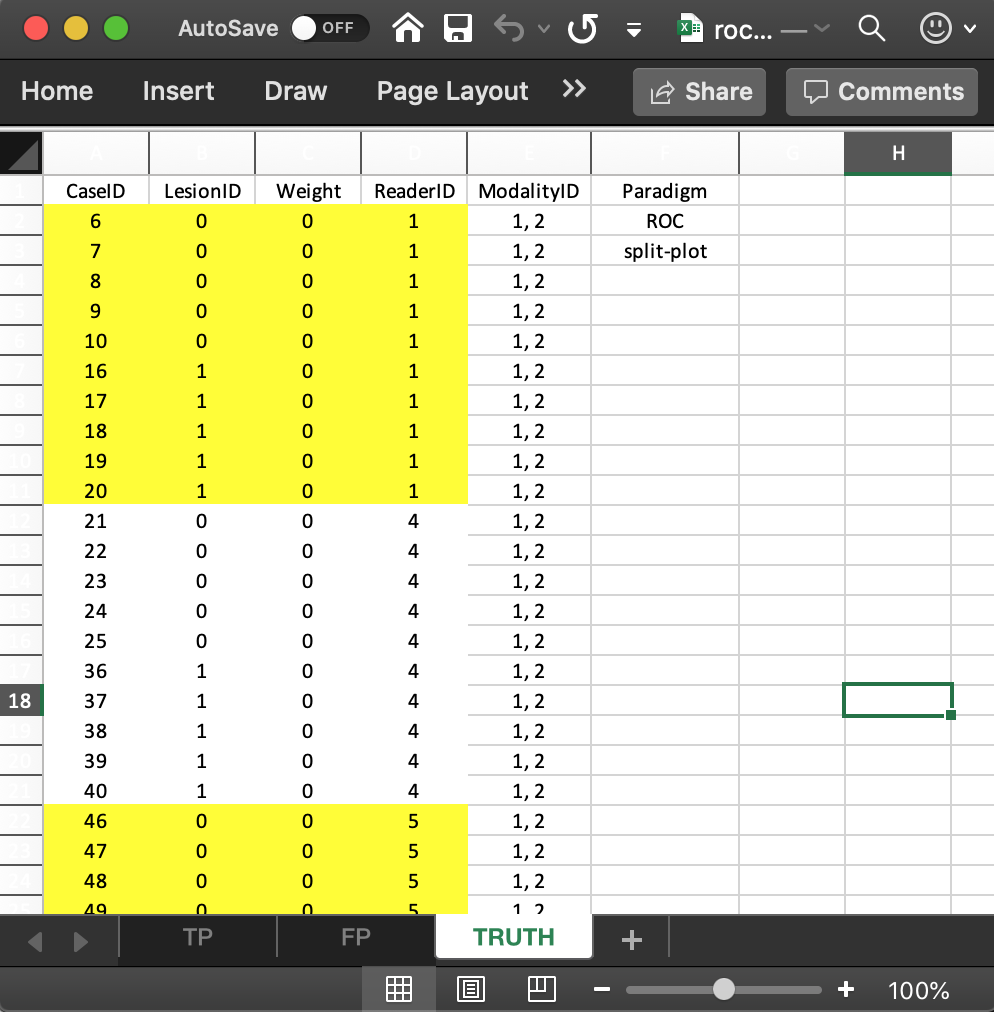
\includegraphics[width=0.5\linewidth,height=0.2\textheight]{images/rocSpTruth} 

}

\caption{Fig. 1: Truth worksheet for file inst/extdata/toyFiles/ROC/rocSp.xlsx}\label{fig:unnamed-chunk-1}
\end{figure}

\hypertarget{the-structure-of-the-roc-split-plot-dataset}{%
\section{The structure of the ROC split plot dataset}\label{the-structure-of-the-roc-split-plot-dataset}}

\begin{itemize}
\tightlist
\item
  The example shown in Fig. 1 corresponds to Excel file \texttt{inst/extdata/toyFiles/ROC/rocSp.xlsx} in the project directory.
\end{itemize}

\begin{Shaded}
\begin{Highlighting}[]
\NormalTok{rocSp <-}\StringTok{ }\KeywordTok{system.file}\NormalTok{(}\StringTok{"extdata"}\NormalTok{, }\StringTok{"toyFiles/ROC/rocSp.xlsx"}\NormalTok{,}
                        \DataTypeTok{package =} \StringTok{"RJafroc"}\NormalTok{, }\DataTypeTok{mustWork =} \OtherTok{TRUE}\NormalTok{)}
\NormalTok{x <-}\StringTok{ }\KeywordTok{DfReadDataFile}\NormalTok{(rocSp, }\DataTypeTok{newExcelFileFormat =} \OtherTok{TRUE}\NormalTok{)}
\KeywordTok{str}\NormalTok{(x)}
\CommentTok{#> List of 12}
\CommentTok{#>  $ NL           : num [1:2, 1:3, 1:30, 1] 1 1 -Inf -Inf -Inf ...}
\CommentTok{#>  $ LL           : num [1:2, 1:3, 1:15, 1] 5 2.3 -Inf -Inf -Inf ...}
\CommentTok{#>  $ lesionVector : int [1:15] 1 1 1 1 1 1 1 1 1 1 ...}
\CommentTok{#>  $ lesionID     : num [1:15, 1] 1 1 1 1 1 1 1 1 1 1 ...}
\CommentTok{#>  $ lesionWeight : num [1:15, 1] 1 1 1 1 1 1 1 1 1 1 ...}
\CommentTok{#>  $ dataType     : chr "ROC"}
\CommentTok{#>  $ modalityID   : Named chr [1:2] "1" "2"}
\CommentTok{#>   ..- attr(*, "names")= chr [1:2] "1" "2"}
\CommentTok{#>  $ readerID     : Named chr [1:3] "1" "4" "5"}
\CommentTok{#>   ..- attr(*, "names")= chr [1:3] "1" "4" "5"}
\CommentTok{#>  $ design       : chr "SPLIT-PLOT"}
\CommentTok{#>  $ normalCases  : int [1:15] 6 7 8 9 10 21 22 23 24 25 ...}
\CommentTok{#>  $ abnormalCases: int [1:15] 16 17 18 19 20 36 37 38 39 40 ...}
\CommentTok{#>  $ truthTableStr: num [1:2, 1:3, 1:30, 1:2] 1 1 NA NA NA NA 1 1 NA NA ...}
\end{Highlighting}
\end{Shaded}

\begin{itemize}
\tightlist
\item
  \texttt{DfReadDataFile()} flag \texttt{newExcelFileFormat} \textbf{must} be set to \texttt{TRUE} for split plot data.
\item
  The dataset object \texttt{x} is a \texttt{list} variable with 12 members.
\item
  There are 15 diseased cases in the dataset (the number of 1's in the \texttt{LesionID} column of the \texttt{Truth} worksheet) and 15 non-diseased cases (the number of 0's in the \texttt{LesionID} column).
\item
  \texttt{x\$NL}, with dimension {[}2, 3, 30, 1{]}, contains the ratings of normal cases. The extra values in the third dimension, filled with \texttt{NAs}, are needed for compatibility with FROC datasets.
\item
  \texttt{x\$LL}, with dimension {[}2, 3, 15, 1{]}, contains the ratings of abnormal cases.
\item
  The \texttt{x\$lesionVector} member is a vector with 15 ones representing the 15 diseased cases in the dataset.
\item
  The \texttt{x\$lesionID} member is an array with 15 ones (this member is needed for compatibility with FROC datasets).
\item
  The \texttt{x\$lesionWeight} member is an array with 15 ones (this member is needed for compatibility with FROC datasets).
\item
  The \texttt{dataType} member is ROC which specifies the data collection method (``ROC'', ``FROC'', ``LROC'' or ``ROI'').
\item
  The \texttt{x\$modalityID} member is a vector with two elements \texttt{"1"} and \texttt{"2"}, naming the two modalities.
\item
  The \texttt{x\$readerID} member is a vector with three elements \texttt{"1"}, \texttt{"4"} and \texttt{"5"}, naming the three modalities.
\item
  The \texttt{x\$design} member is SPLIT-PLOT; specifies the dataset design, which can be either ``CROSSED'' or ``SPLIT-PLOT''.
\item
  The \texttt{x\$normalCases} member lists the names of the normal cases, 6, 7, 8, 9, 10, 21, 22, 23, 24, 25, 46, 47, 48, 49, 50.
\item
  The \texttt{x\$abnormalCases} member lists the names of the abnormal cases, 16, 17, 18, 19, 20, 36, 37, 38, 39, 40, 51, 52, 53, 54, 55.
\item
  The \texttt{x\$truthTableStr} member quantifies the structure of the dataset, as explained next. \textbf{It is used in the \texttt{DfReadDataFile()} function to check for data entry errors.}
\end{itemize}

\hypertarget{the-truthtablestr-member}{%
\section{\texorpdfstring{The \texttt{truthTableStr} member}{The truthTableStr member}}\label{the-truthtablestr-member}}

\begin{itemize}
\tightlist
\item
  This is a \texttt{2\ x\ 3\ x\ 30\ x\ 2} array, i.e., I x J x K x (maximum number of lesions per case plus 1). The \texttt{plus\ 1} is needed to accommodate normal cases with \texttt{lesionID} = 0. {[}Zero is not a valid array subscript in \texttt{R}.{]}
\item
  Each entry in this array is either \texttt{1}, meaning the corresponding interpretation exists, or \texttt{NA}, meaning the corresponding interpretation does not exist.
\item
  For example, \texttt{x\$truthTableStr{[}1,1,1,1{]}} is 1. This means that an interpretation exists for the first treatment (\texttt{modalityID} = 1), first reader (\texttt{readerID} = 1) and first (normal) case (\texttt{caseID} = 6 and \texttt{lesionID} = 0). This example corresponds to row 2 in the \texttt{TRUTH} worksheet.
\item
  The following shows that the first reader interprets the first five normal cases in both modalities.
\end{itemize}

\begin{Shaded}
\begin{Highlighting}[]
\NormalTok{x}\OperatorTok{$}\NormalTok{truthTableStr[,}\DecValTok{1}\NormalTok{,}\DecValTok{1}\OperatorTok{:}\DecValTok{15}\NormalTok{,}\DecValTok{1}\NormalTok{]}
\CommentTok{#>      [,1] [,2] [,3] [,4] [,5] [,6] [,7] [,8] [,9] [,10] [,11] [,12] [,13] [,14]}
\CommentTok{#> [1,]    1    1    1    1    1   NA   NA   NA   NA    NA    NA    NA    NA    NA}
\CommentTok{#> [2,]    1    1    1    1    1   NA   NA   NA   NA    NA    NA    NA    NA    NA}
\CommentTok{#>      [,15]}
\CommentTok{#> [1,]    NA}
\CommentTok{#> [2,]    NA}
\end{Highlighting}
\end{Shaded}

\begin{itemize}
\tightlist
\item
  In the following all elements are \texttt{NA} because normal cases correspond to lesionID = 1.
\end{itemize}

\begin{Shaded}
\begin{Highlighting}[]
\NormalTok{x}\OperatorTok{$}\NormalTok{truthTableStr[,}\DecValTok{1}\NormalTok{,}\DecValTok{1}\OperatorTok{:}\DecValTok{15}\NormalTok{,}\DecValTok{2}\NormalTok{]}
\CommentTok{#>      [,1] [,2] [,3] [,4] [,5] [,6] [,7] [,8] [,9] [,10] [,11] [,12] [,13] [,14]}
\CommentTok{#> [1,]   NA   NA   NA   NA   NA   NA   NA   NA   NA    NA    NA    NA    NA    NA}
\CommentTok{#> [2,]   NA   NA   NA   NA   NA   NA   NA   NA   NA    NA    NA    NA    NA    NA}
\CommentTok{#>      [,15]}
\CommentTok{#> [1,]    NA}
\CommentTok{#> [2,]    NA}
\end{Highlighting}
\end{Shaded}

\begin{itemize}
\tightlist
\item
  The following shows that the second reader interprets the next group of five normal cases, indexed 6 through 10, in both modalities.
\end{itemize}

\begin{Shaded}
\begin{Highlighting}[]
\NormalTok{x}\OperatorTok{$}\NormalTok{truthTableStr[,}\DecValTok{2}\NormalTok{,}\DecValTok{1}\OperatorTok{:}\DecValTok{15}\NormalTok{,}\DecValTok{1}\NormalTok{]}
\CommentTok{#>      [,1] [,2] [,3] [,4] [,5] [,6] [,7] [,8] [,9] [,10] [,11] [,12] [,13] [,14]}
\CommentTok{#> [1,]   NA   NA   NA   NA   NA    1    1    1    1     1    NA    NA    NA    NA}
\CommentTok{#> [2,]   NA   NA   NA   NA   NA    1    1    1    1     1    NA    NA    NA    NA}
\CommentTok{#>      [,15]}
\CommentTok{#> [1,]    NA}
\CommentTok{#> [2,]    NA}
\end{Highlighting}
\end{Shaded}

\begin{itemize}
\tightlist
\item
  The following shows that the third reader interprets the next group of five normal cases, indexed 11 through 15, in both modalities.
\end{itemize}

\begin{Shaded}
\begin{Highlighting}[]
\NormalTok{x}\OperatorTok{$}\NormalTok{truthTableStr[,}\DecValTok{3}\NormalTok{,}\DecValTok{1}\OperatorTok{:}\DecValTok{15}\NormalTok{,}\DecValTok{1}\NormalTok{]}
\CommentTok{#>      [,1] [,2] [,3] [,4] [,5] [,6] [,7] [,8] [,9] [,10] [,11] [,12] [,13] [,14]}
\CommentTok{#> [1,]   NA   NA   NA   NA   NA   NA   NA   NA   NA    NA     1     1     1     1}
\CommentTok{#> [2,]   NA   NA   NA   NA   NA   NA   NA   NA   NA    NA     1     1     1     1}
\CommentTok{#>      [,15]}
\CommentTok{#> [1,]     1}
\CommentTok{#> [2,]     1}
\end{Highlighting}
\end{Shaded}

\begin{itemize}
\tightlist
\item
  The following shows that the first reader interprets the first group of five abnormal cases, indexed 16 through 20, in both modalities.
\end{itemize}

\begin{Shaded}
\begin{Highlighting}[]
\NormalTok{x}\OperatorTok{$}\NormalTok{truthTableStr[,}\DecValTok{1}\NormalTok{,}\DecValTok{16}\OperatorTok{:}\DecValTok{30}\NormalTok{,}\DecValTok{2}\NormalTok{]}
\CommentTok{#>      [,1] [,2] [,3] [,4] [,5] [,6] [,7] [,8] [,9] [,10] [,11] [,12] [,13] [,14]}
\CommentTok{#> [1,]    1    1    1    1    1   NA   NA   NA   NA    NA    NA    NA    NA    NA}
\CommentTok{#> [2,]    1    1    1    1    1   NA   NA   NA   NA    NA    NA    NA    NA    NA}
\CommentTok{#>      [,15]}
\CommentTok{#> [1,]    NA}
\CommentTok{#> [2,]    NA}
\end{Highlighting}
\end{Shaded}

\begin{itemize}
\tightlist
\item
  In the following all elements are \texttt{NA} because abnormal cases correspond to \texttt{lesionID} = 2.
\end{itemize}

\begin{Shaded}
\begin{Highlighting}[]
\NormalTok{x}\OperatorTok{$}\NormalTok{truthTableStr[,}\DecValTok{1}\NormalTok{,}\DecValTok{16}\OperatorTok{:}\DecValTok{30}\NormalTok{,}\DecValTok{1}\NormalTok{]}
\CommentTok{#>      [,1] [,2] [,3] [,4] [,5] [,6] [,7] [,8] [,9] [,10] [,11] [,12] [,13] [,14]}
\CommentTok{#> [1,]   NA   NA   NA   NA   NA   NA   NA   NA   NA    NA    NA    NA    NA    NA}
\CommentTok{#> [2,]   NA   NA   NA   NA   NA   NA   NA   NA   NA    NA    NA    NA    NA    NA}
\CommentTok{#>      [,15]}
\CommentTok{#> [1,]    NA}
\CommentTok{#> [2,]    NA}
\end{Highlighting}
\end{Shaded}

\begin{figure}

{\centering 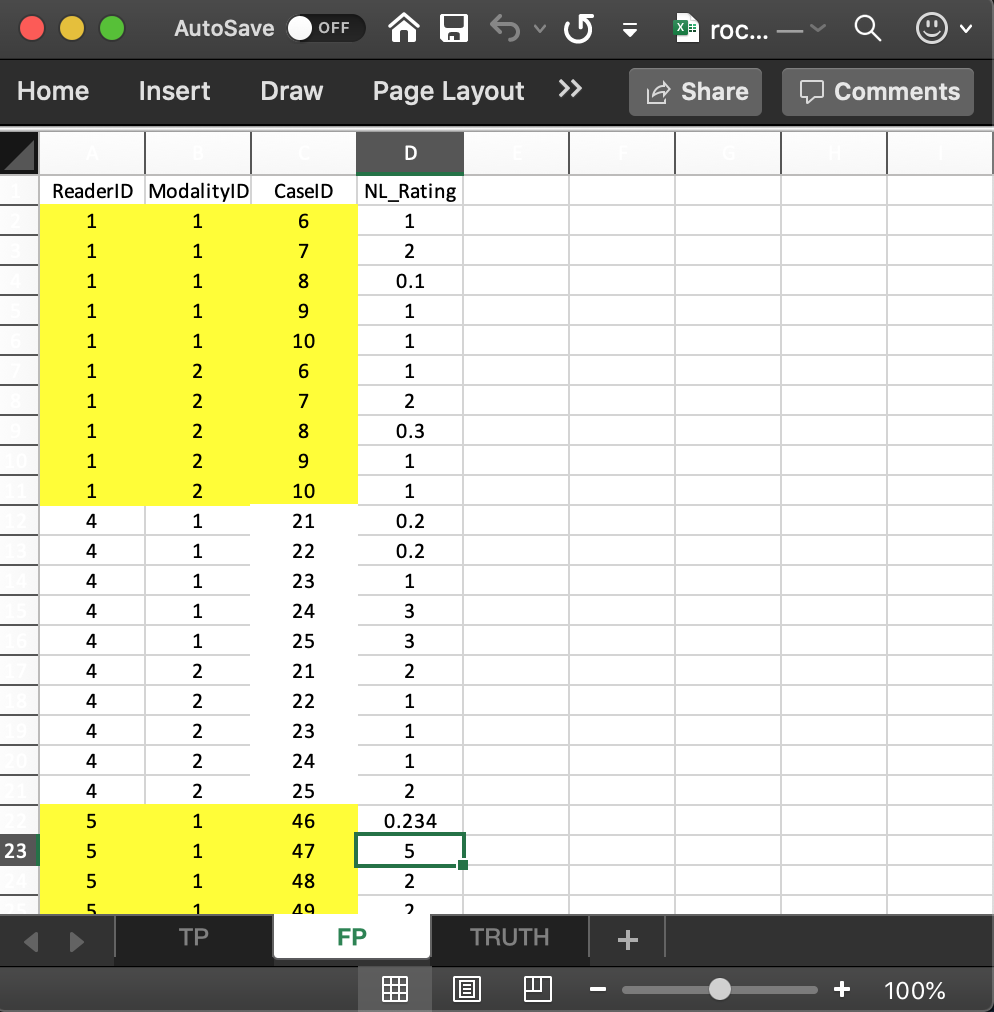
\includegraphics[width=0.5\linewidth,height=0.2\textheight]{images/rocSpFp} 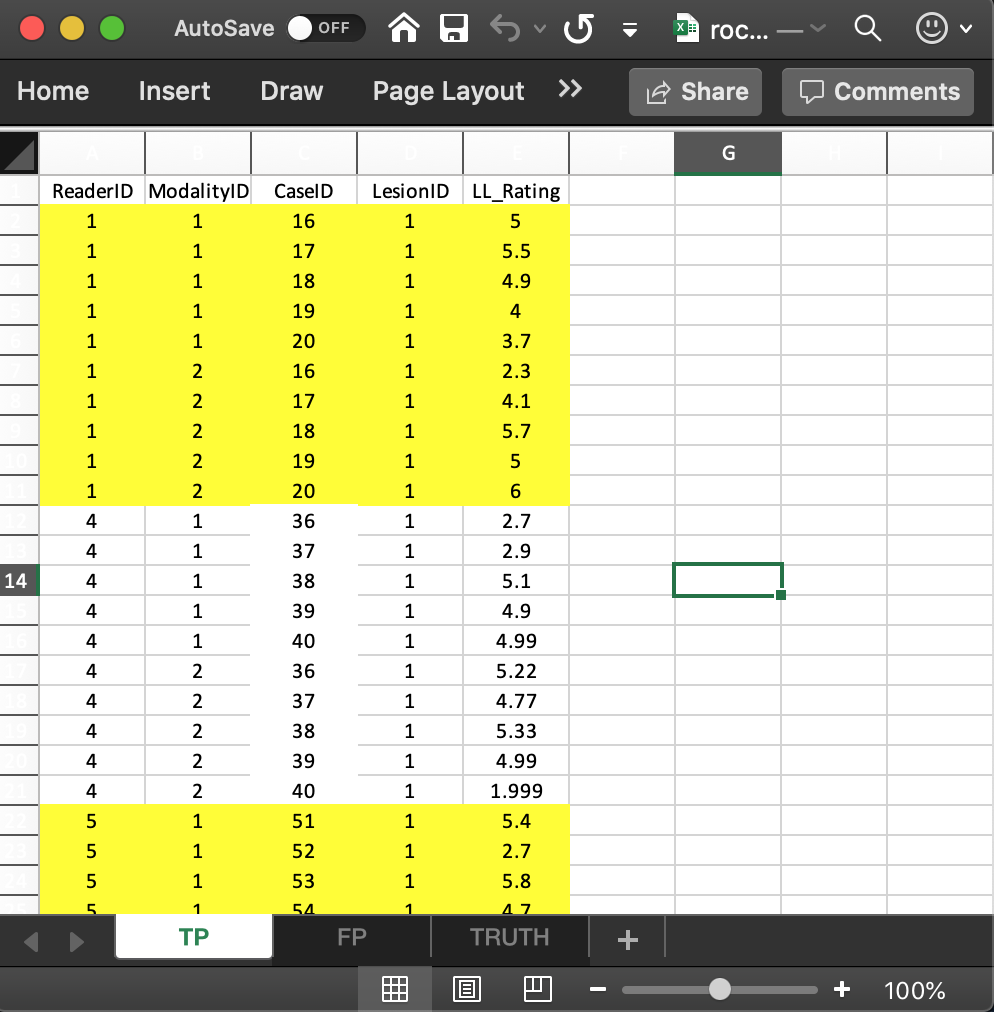
\includegraphics[width=0.5\linewidth,height=0.2\textheight]{images/rocSpTp} 

}

\caption{Fig. 2 FP/TP worksheets; LEFT=FP, (b) RIGHT=TP}\label{fig:unnamed-chunk-9}
\end{figure}

\hypertarget{the-false-positive-fp-ratings-2}{%
\section{The false positive (FP) ratings}\label{the-false-positive-fp-ratings-2}}

\begin{itemize}
\tightlist
\item
  These are found in the \texttt{FP} or \texttt{NL} worksheet, see Fig. 2, left panel.
\item
  This worksheet has the ratings of non-diseased cases.
\item
  The common vertical length is 30 in this example (2 modalities times 3 readers times 5 non-diseased cases per reader).
\item
  \texttt{ReaderID}: the reader labels: these must be from \texttt{1}, \texttt{4} or \texttt{5}, as declared in the \texttt{Truth} worksheet.
\item
  \texttt{ModalityID}: the modality labels: \texttt{1} or \texttt{2}, as declared in the \texttt{Truth} worksheet.
\item
  \texttt{CaseID}: the labels of non-diseased cases. Each \texttt{CaseID} - \texttt{ReaderID} combination must be consistent with that declared in the \texttt{Truth} worsheet.\\
\item
  \texttt{NL\_Rating}: the floating point ratings of non-diseased cases. Each row of this worksheet yields a rating corresponding to the values of \texttt{ReaderID}, \texttt{ModalityID} and \texttt{CaseID} for that row.
\end{itemize}

\begin{Shaded}
\begin{Highlighting}[]
\NormalTok{x}\OperatorTok{$}\NormalTok{NL[,}\DecValTok{1}\NormalTok{,}\DecValTok{1}\OperatorTok{:}\DecValTok{15}\NormalTok{,}\DecValTok{1}\NormalTok{]}
\CommentTok{#>      [,1] [,2] [,3] [,4] [,5] [,6] [,7] [,8] [,9] [,10] [,11] [,12] [,13] [,14]}
\CommentTok{#> [1,]    1    2  0.1    1    1 -Inf -Inf -Inf -Inf  -Inf  -Inf  -Inf  -Inf  -Inf}
\CommentTok{#> [2,]    1    2  0.3    1    1 -Inf -Inf -Inf -Inf  -Inf  -Inf  -Inf  -Inf  -Inf}
\CommentTok{#>      [,15]}
\CommentTok{#> [1,]  -Inf}
\CommentTok{#> [2,]  -Inf}
\NormalTok{x}\OperatorTok{$}\NormalTok{NL[,}\DecValTok{2}\NormalTok{,}\DecValTok{1}\OperatorTok{:}\DecValTok{15}\NormalTok{,}\DecValTok{1}\NormalTok{]}
\CommentTok{#>      [,1] [,2] [,3] [,4] [,5] [,6] [,7] [,8] [,9] [,10] [,11] [,12] [,13] [,14]}
\CommentTok{#> [1,] -Inf -Inf -Inf -Inf -Inf  0.2  0.2    1    3     3  -Inf  -Inf  -Inf  -Inf}
\CommentTok{#> [2,] -Inf -Inf -Inf -Inf -Inf  2.0  1.0    1    1     2  -Inf  -Inf  -Inf  -Inf}
\CommentTok{#>      [,15]}
\CommentTok{#> [1,]  -Inf}
\CommentTok{#> [2,]  -Inf}
\NormalTok{x}\OperatorTok{$}\NormalTok{NL[,}\DecValTok{3}\NormalTok{,}\DecValTok{1}\OperatorTok{:}\DecValTok{15}\NormalTok{,}\DecValTok{1}\NormalTok{]}
\CommentTok{#>      [,1] [,2] [,3] [,4] [,5] [,6] [,7] [,8] [,9] [,10] [,11] [,12] [,13] [,14]}
\CommentTok{#> [1,] -Inf -Inf -Inf -Inf -Inf -Inf -Inf -Inf -Inf  -Inf 0.234     5     2     2}
\CommentTok{#> [2,] -Inf -Inf -Inf -Inf -Inf -Inf -Inf -Inf -Inf  -Inf 3.000     2     2     2}
\CommentTok{#>      [,15]}
\CommentTok{#> [1,]  2.00}
\CommentTok{#> [2,]  0.33}
\end{Highlighting}
\end{Shaded}

\begin{itemize}
\tightlist
\item
  The first line of the above code shows the ratings, in both modalities, of the first five non-diseased cases with \texttt{CaseID}s \texttt{6,7,8,9,10} (indexed 1, 2, 3, 4, 5 and appearing in the first five columns) interpreted by the first reader (\texttt{ReaderID} 1).
\item
  The second line shows the ratings, in both modalities, of the next five non-diseased cases with \texttt{CaseID}s \texttt{21,22,23,24,25} (indexed 6, 7, 8, 9, 10and appearing in the next five columns) interpreted by the second reader (\texttt{ReaderID} 4).
\item
  The third line shows the ratings, in both modalities, of the final five non-diseased cases with \texttt{CaseID}s \texttt{46,47,48,49,50} (indexed 11, 12, 13, 14, 15and appearing in the final five columns) interpreted by the third reader (\texttt{ReaderID} 5).
\item
  Values such as \texttt{x\$NL{[},,16:30,1{]}}, which are there for compatibility with FROC data, are all filled with \texttt{-Inf}.
\end{itemize}

\hypertarget{the-true-positive-tp-ratings-2}{%
\section{The true positive (TP) ratings}\label{the-true-positive-tp-ratings-2}}

\begin{itemize}
\tightlist
\item
  These are found in the \texttt{TP} or \texttt{LL} worksheet, see Fig. 2, right panel.
\item
  This worksheet has the ratings of diseased cases.
\item
  The common vertical length is 30 in this example (2 modalities times 3 readers times 5 diseased cases per reader).
\item
  \texttt{ReaderID}: the reader labels: these must be from \texttt{1}, \texttt{4} or \texttt{5}, as declared in the \texttt{Truth} worksheet.
\item
  \texttt{ModalityID}: the modality labels: \texttt{1} or \texttt{2}, as declared in the \texttt{Truth} worksheet.
\item
  \texttt{CaseID}: the labels of diseased cases. Each \texttt{CaseID} - \texttt{ReaderID} combination must be consistent with that declared in the \texttt{Truth} worsheet.\\
\item
  \texttt{LL\_Rating}: the floating point ratings of diseased cases. Each row of this worksheet yields a rating corresponding to the values of \texttt{ReaderID}, \texttt{ModalityID} and \texttt{CaseID} for that row.
\end{itemize}

\begin{Shaded}
\begin{Highlighting}[]
\NormalTok{x}\OperatorTok{$}\NormalTok{LL[,}\DecValTok{1}\NormalTok{,}\DecValTok{1}\OperatorTok{:}\DecValTok{15}\NormalTok{,}\DecValTok{1}\NormalTok{]}
\CommentTok{#>      [,1] [,2] [,3] [,4] [,5] [,6] [,7] [,8] [,9] [,10] [,11] [,12] [,13] [,14]}
\CommentTok{#> [1,]  5.0  5.5  4.9    4  3.7 -Inf -Inf -Inf -Inf  -Inf  -Inf  -Inf  -Inf  -Inf}
\CommentTok{#> [2,]  2.3  4.1  5.7    5  6.0 -Inf -Inf -Inf -Inf  -Inf  -Inf  -Inf  -Inf  -Inf}
\CommentTok{#>      [,15]}
\CommentTok{#> [1,]  -Inf}
\CommentTok{#> [2,]  -Inf}
\NormalTok{x}\OperatorTok{$}\NormalTok{LL[,}\DecValTok{2}\NormalTok{,}\DecValTok{1}\OperatorTok{:}\DecValTok{15}\NormalTok{,}\DecValTok{1}\NormalTok{]}
\CommentTok{#>      [,1] [,2] [,3] [,4] [,5] [,6] [,7] [,8] [,9] [,10] [,11] [,12] [,13] [,14]}
\CommentTok{#> [1,] -Inf -Inf -Inf -Inf -Inf 2.70 2.90 5.10 4.90 4.990  -Inf  -Inf  -Inf  -Inf}
\CommentTok{#> [2,] -Inf -Inf -Inf -Inf -Inf 5.22 4.77 5.33 4.99 1.999  -Inf  -Inf  -Inf  -Inf}
\CommentTok{#>      [,15]}
\CommentTok{#> [1,]  -Inf}
\CommentTok{#> [2,]  -Inf}
\NormalTok{x}\OperatorTok{$}\NormalTok{LL[,}\DecValTok{3}\NormalTok{,}\DecValTok{1}\OperatorTok{:}\DecValTok{15}\NormalTok{,}\DecValTok{1}\NormalTok{]}
\CommentTok{#>      [,1] [,2] [,3] [,4] [,5] [,6] [,7] [,8] [,9] [,10] [,11] [,12] [,13] [,14]}
\CommentTok{#> [1,] -Inf -Inf -Inf -Inf -Inf -Inf -Inf -Inf -Inf  -Inf   5.4   2.7   5.8   4.7}
\CommentTok{#> [2,] -Inf -Inf -Inf -Inf -Inf -Inf -Inf -Inf -Inf  -Inf   5.4   2.7   5.8   4.7}
\CommentTok{#>      [,15]}
\CommentTok{#> [1,]     5}
\CommentTok{#> [2,]     5}
\end{Highlighting}
\end{Shaded}

\begin{itemize}
\tightlist
\item
  The first line of code shows the ratings, in both modalities, of the first five diseased cases with \texttt{CaseID}s \texttt{16,17,18,19,20} (indexed 1, 2, 3, 4, 5and appearing in the first five columns) interpreted by the first reader (\texttt{ReaderID} 1).
\item
  The second line shows the ratings, in both modalities, of the next five diseased cases with \texttt{CaseID}s \texttt{36,37,38,39,40} (indexed 6, 7, 8, 9, 10and appearing in the next five columns) interpreted by the second reader (\texttt{ReaderID} 4).
\item
  The third line shows the ratings, in both modalities, of the final five non-diseased cases with \texttt{CaseID}s \texttt{51,52,53,54,55} (indexed 11, 12, 13, 14, 15and appearing in the final five columns) interpreted by the third reader (\texttt{ReaderID} 5).
\end{itemize}

\hypertarget{summary-1}{%
\section{Summary}\label{summary-1}}

\begin{itemize}
\tightlist
\item
  The FROC dataset has far less regularity in structure as compared to an ROC dataset.
\item
  The length of the first dimension of either \texttt{x\$NL} or \texttt{x\$LL} list members is the total number of modalities, 2 in the current example.
\item
  The length of the second dimension of either \texttt{x\$NL} or \texttt{x\$LL} list members is the total number of readers, 3 in the current example.
\item
  The length of the third dimension of \texttt{x\$NL} is the total number of cases, 8 in the current example. The first three positions account for \texttt{NL} marks on non-diseased cases and the remaining 5 positions account for \texttt{NL} marks on diseased cases.
\item
  The length of the third dimension of \texttt{x\$LL} is the total number of diseased cases, 5 in the current example.
\item
  The length of the fourth dimension of \texttt{x\$NL} is determined by the case (diseased or non-diseased) with the most \texttt{NL} marks, 2 in the current example.
\item
  The length of the fourth dimension of \texttt{x\$LL} is determined by the diseased case with the most lesions, 3 in the current example.
\end{itemize}

\hypertarget{references-3}{%
\section{References}\label{references-3}}

\hypertarget{part-split-plot-datasets}{%
\part*{SPLIT-PLOT DATASETS}\label{part-split-plot-datasets}}
\addcontentsline{toc}{part}{SPLIT-PLOT DATASETS}

\hypertarget{frocSpdataformat}{%
\chapter{FROC ROC DATA FORMAT SPLIT PLOT}\label{frocSpdataformat}}

\hypertarget{introduction-3}{%
\section{Introduction}\label{introduction-3}}

\begin{itemize}
\tightlist
\item
  The purpose of this vignette is to explain the data format of the input Excel file for an FROC \emph{split-plot} dataset.
\item
  In a split-plot dataset each reader interprets a sub-set of cases in all modalities.
\item
  The cases interpreted by different readers have no overlap.
\item
  It is assumed, for now, that each sub-set of cases has the same numbers of non-diseased and diseased cases.
\end{itemize}

\hypertarget{the-excel-data-format-3}{%
\section{The Excel data format}\label{the-excel-data-format-3}}

The Excel file has three worsheets named \texttt{Truth}, \texttt{NL} or \texttt{FP} and \texttt{LL} or \texttt{TP}.

\hypertarget{the-truth-worksheet-3}{%
\section{\texorpdfstring{The \texttt{Truth} worksheet}{The Truth worksheet}}\label{the-truth-worksheet-3}}

The \texttt{Truth} worksheet contains 6 columns: \texttt{CaseID}, \texttt{LesionID}, \texttt{Weight}, \texttt{ReaderID}, \texttt{ModalityID} and \texttt{Paradigm}.

\begin{itemize}
\tightlist
\item
  The first five columns contain as many rows as there are non-diseased cases (9) plus total number of lesions (27) in the dataset (each row with a non-zero \texttt{LesionID} corresponds to a lesion).
\item
  \texttt{CaseID}: unique \textbf{integers}, one per case, representing the cases in the dataset.
\item
  \texttt{LesionID}: integers 0, 1, 2, etc., with each 0 representing a non-diseased case, 1 representing the \emph{first} lesion on a diseased case, 2 representing the second lesion on a diseased case, if present, and so on.
\item
  The three non-diseased cases interpreted by reader with \texttt{ReaderID} value \texttt{0} are labeled \texttt{1}, \texttt{2}, \texttt{3}, while the diseased cases interpreted by this reader are labeled \texttt{70}, \texttt{71}, \texttt{72}, \texttt{73} and \texttt{74}, with \texttt{LesionID} values ranging from 1 to 3.\\
\item
  The second reader, with \texttt{ReaderID} value \texttt{1}, interprets three non-diseased cases labeled \texttt{4}, \texttt{5} and \texttt{6}, each with \texttt{LesionID} value \texttt{0}, and five diseased cases labeled \texttt{80}, \texttt{81}, \texttt{82}, \texttt{83} and \texttt{84}, with \texttt{LesionID} values ranging from 1 to 3.\\
\item
  The third reader, with \texttt{ReaderID} value \texttt{2}, interprets three non-diseased cases labeled \texttt{7}, \texttt{8} and \texttt{9}, each with \texttt{LesionID} value \texttt{0} and five diseased cases labeled \texttt{90}, \texttt{91}, \texttt{92}, \texttt{93} and \texttt{94}, with \texttt{LesionID} values ranging from 1 to 3.\\
\item
  \texttt{Weight}: floating point value adding upto unity for diseased cases as required for FROC data.
\item
  \texttt{ModalityID}: a comma-separated listing of modalities, each represented by a unique \textbf{integer}. In the example shown below each cell has the value \texttt{0,\ 1}. \textbf{Each cell has to be text formatted.}
\item
  \texttt{Paradigm}: In the example shown below, the contents are \texttt{FROC} and \texttt{split-plot}.
\end{itemize}

\begin{figure}

{\centering 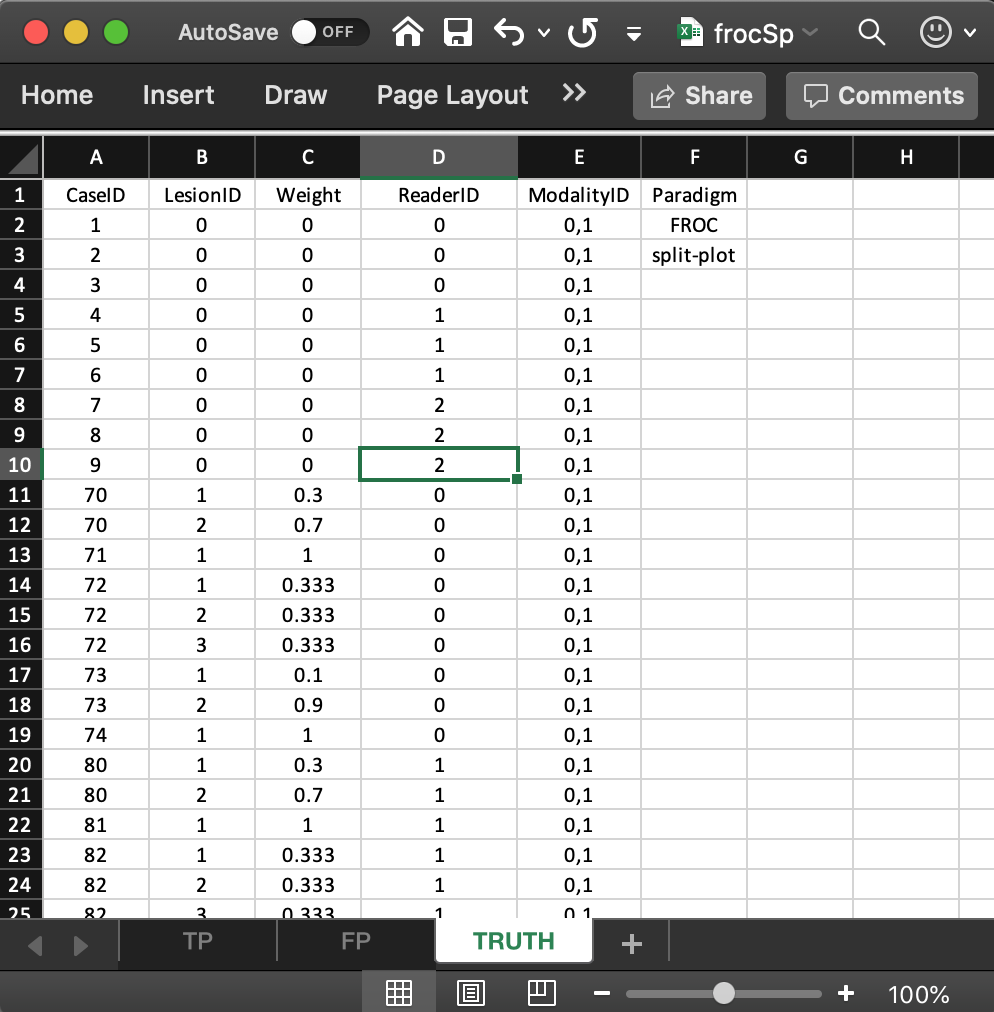
\includegraphics[width=0.5\linewidth,height=0.2\textheight]{images/frocSpTruth} 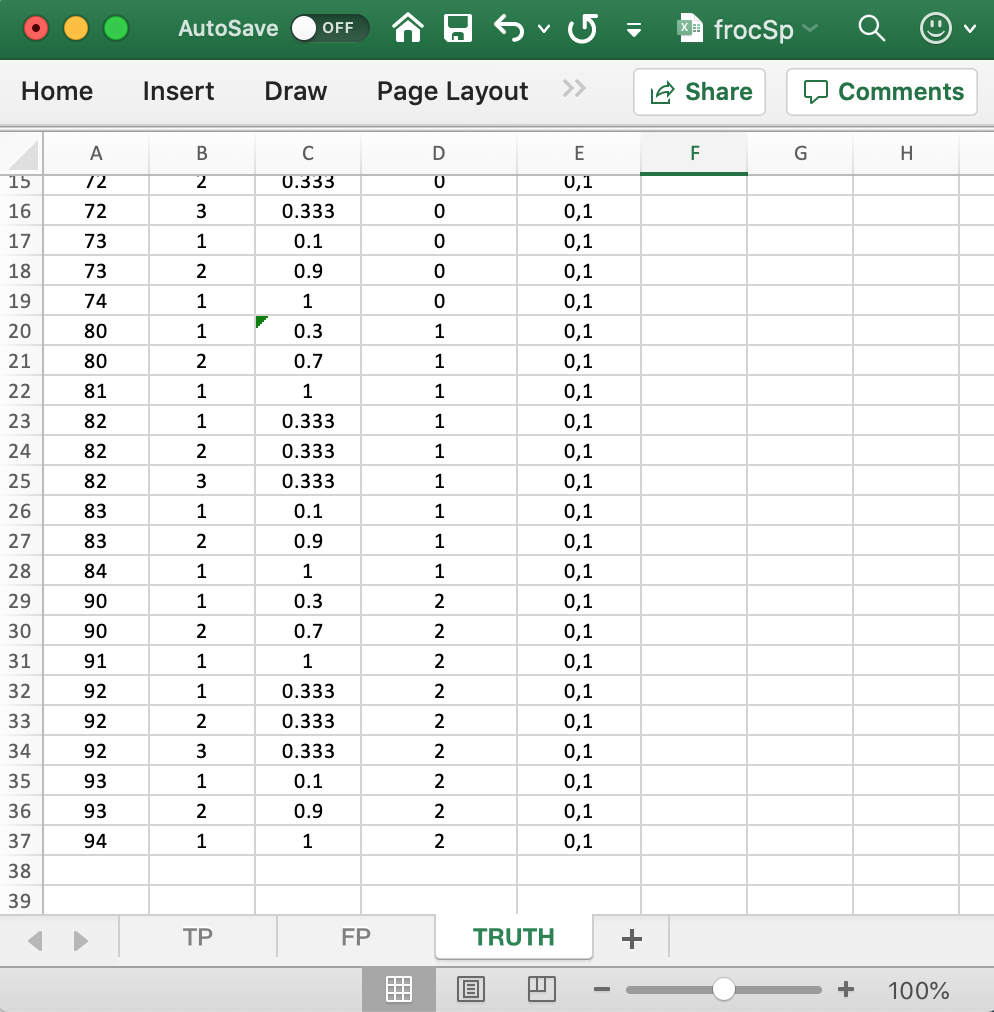
\includegraphics[width=0.5\linewidth,height=0.2\textheight]{images/frocSpTruth2} 

}

\caption{Two views of Truth worksheet for file frocSp.xlsx}\label{fig:frocSpTruth2}
\end{figure}

\hypertarget{the-structure-of-the-froc-split-plot-dataset}{%
\section{The structure of the FROC split plot dataset}\label{the-structure-of-the-froc-split-plot-dataset}}

The example shown in Fig. 1 corresponds to Excel file \texttt{inst/extdata/toyFiles/FROC/frocSp.xlsx} in the project directory.

\begin{Shaded}
\begin{Highlighting}[]
\NormalTok{frocSp <-}\StringTok{ }\KeywordTok{system.file}\NormalTok{(}\StringTok{"extdata"}\NormalTok{, }\StringTok{"toyFiles/FROC/frocSp.xlsx"}\NormalTok{,}
                        \DataTypeTok{package =} \StringTok{"RJafroc"}\NormalTok{, }\DataTypeTok{mustWork =} \OtherTok{TRUE}\NormalTok{)}
\NormalTok{x <-}\StringTok{ }\KeywordTok{DfReadDataFile}\NormalTok{(frocSp, }\DataTypeTok{newExcelFileFormat =} \OtherTok{TRUE}\NormalTok{)}
\KeywordTok{str}\NormalTok{(x)}
\CommentTok{#> List of 12}
\CommentTok{#>  $ NL           : num [1:2, 1:3, 1:24, 1:3] 1.02 2.89 -Inf -Inf -Inf ...}
\CommentTok{#>  $ LL           : num [1:2, 1:3, 1:15, 1:3] 5.28 5.2 -Inf -Inf -Inf ...}
\CommentTok{#>  $ lesionVector : int [1:15] 2 1 3 2 1 2 1 3 2 1 ...}
\CommentTok{#>  $ lesionID     : num [1:15, 1:3] 1 1 1 1 1 1 1 1 1 1 ...}
\CommentTok{#>  $ lesionWeight : num [1:15, 1:3] 0.3 1 0.333 0.1 1 ...}
\CommentTok{#>  $ dataType     : chr "FROC"}
\CommentTok{#>  $ modalityID   : Named chr [1:2] "0" "1"}
\CommentTok{#>   ..- attr(*, "names")= chr [1:2] "0" "1"}
\CommentTok{#>  $ readerID     : Named chr [1:3] "0" "1" "2"}
\CommentTok{#>   ..- attr(*, "names")= chr [1:3] "0" "1" "2"}
\CommentTok{#>  $ design       : chr "SPLIT-PLOT"}
\CommentTok{#>  $ normalCases  : int [1:9] 1 2 3 4 5 6 7 8 9}
\CommentTok{#>  $ abnormalCases: int [1:15] 70 71 72 73 74 80 81 82 83 84 ...}
\CommentTok{#>  $ truthTableStr: num [1:2, 1:3, 1:24, 1:4] 1 1 NA NA NA NA 1 1 NA NA ...}
\end{Highlighting}
\end{Shaded}

\begin{itemize}
\tightlist
\item
  Flag \texttt{newExcelFileFormat} \textbf{must} be set to \texttt{TRUE} for split plot data.
\item
  The dataset object \texttt{x} is a \texttt{list} variable with 12 members.
\item
  Note that the \texttt{dataType} member is FROC and the \texttt{design} member is SPLIT-PLOT.
\item
  There are 15 diseased cases in the dataset (the number of 1's in the \texttt{LesionID} column of the \texttt{Truth} worksheet) and 9 non-diseased cases (the number of 0's in the \texttt{LesionID} column).
\item
  The \texttt{x\$lesionVector} member is a vector with 15 ones representing the 15 diseased cases in the dataset.
\item
  The \texttt{x\$lesionID} member is a 15 x 3 array labeling the lesions in the dataset.
\item
  The \texttt{x\$lesionWeight} member is a 15 x 3 array.
\end{itemize}

\begin{Shaded}
\begin{Highlighting}[]
\NormalTok{x}\OperatorTok{$}\NormalTok{lesionVector}
\CommentTok{#>  [1] 2 1 3 2 1 2 1 3 2 1 2 1 3 2 1}
\NormalTok{x}\OperatorTok{$}\NormalTok{lesionID}
\CommentTok{#>       [,1] [,2] [,3]}
\CommentTok{#>  [1,]    1    2 -Inf}
\CommentTok{#>  [2,]    1 -Inf -Inf}
\CommentTok{#>  [3,]    1    2    3}
\CommentTok{#>  [4,]    1    2 -Inf}
\CommentTok{#>  [5,]    1 -Inf -Inf}
\CommentTok{#>  [6,]    1    2 -Inf}
\CommentTok{#>  [7,]    1 -Inf -Inf}
\CommentTok{#>  [8,]    1    2    3}
\CommentTok{#>  [9,]    1    2 -Inf}
\CommentTok{#> [10,]    1 -Inf -Inf}
\CommentTok{#> [11,]    1    2 -Inf}
\CommentTok{#> [12,]    1 -Inf -Inf}
\CommentTok{#> [13,]    1    2    3}
\CommentTok{#> [14,]    1    2 -Inf}
\CommentTok{#> [15,]    1 -Inf -Inf}
\NormalTok{x}\OperatorTok{$}\NormalTok{lesionWeight}
\CommentTok{#>            [,1]      [,2]      [,3]}
\CommentTok{#>  [1,] 0.3000000 0.7000000      -Inf}
\CommentTok{#>  [2,] 1.0000000      -Inf      -Inf}
\CommentTok{#>  [3,] 0.3333333 0.3333333 0.3333333}
\CommentTok{#>  [4,] 0.1000000 0.9000000      -Inf}
\CommentTok{#>  [5,] 1.0000000      -Inf      -Inf}
\CommentTok{#>  [6,] 0.3000000 0.7000000      -Inf}
\CommentTok{#>  [7,] 1.0000000      -Inf      -Inf}
\CommentTok{#>  [8,] 0.3333333 0.3333333 0.3333333}
\CommentTok{#>  [9,] 0.1000000 0.9000000      -Inf}
\CommentTok{#> [10,] 1.0000000      -Inf      -Inf}
\CommentTok{#> [11,] 0.3000000 0.7000000      -Inf}
\CommentTok{#> [12,] 1.0000000      -Inf      -Inf}
\CommentTok{#> [13,] 0.3333333 0.3333333 0.3333333}
\CommentTok{#> [14,] 0.1000000 0.9000000      -Inf}
\CommentTok{#> [15,] 1.0000000      -Inf      -Inf}
\end{Highlighting}
\end{Shaded}

\begin{itemize}
\tightlist
\item
  The \texttt{x\$truthTableStr} member is a \texttt{2\ x\ 3\ x\ 24\ x\ 4} array, i.e., I x J x K x (maximum number of lesions per case plus 1). The \texttt{plus\ 1} is needed to accommodate normal cases with \texttt{lesionID} = 0.
\item
  Each entry in this array is either \texttt{1}, meaning the corresponding interpretation exists, or \texttt{NA}, meaning the corresponding interpretation does not exist.
\item
  For example, \texttt{x\$truthTableStr{[}1,1,1,1{]}} is 1. This means that an interpretation exists for the first treatment (\texttt{modalityID} = 0), first reader (\texttt{readerID} = 0) and first (normal) case \texttt{caseID} = 1 and \texttt{lesionID} = 0. This example corresponds to row 2 in the \texttt{TRUTH} worksheet.
\item
  \texttt{x\$truthTableStr{[}1,1,4,1{]}} is NA, which means an interpretation does not exist for the first treatment, first reader and fourth (normal) case.
\item
  However, \texttt{x\$truthTableStr{[}1,2,4,1{]}} is 1, which means an interpretation does exist for the first treatment, second reader and fourth (normal) case. This example corresponds to row 5 in the \texttt{TRUTH} worksheet.
\item
  Likewise, \texttt{x\$truthTableStr{[}1,1,10,3{]}} is 1, which means an interpretation does exist for the first treatment, first reader, tenth (abnormal) case and \texttt{lesionID} = 2. This example corresponds to row 12 in the \texttt{TRUTH} worksheet.
\item
  As an aside, in the FROC paradigm an interpretation need not yield a mark-rating pair. An interpretation means the reader was ``exposed to'' and had the opportunity to mark the corresponding treatment-reader-case-lesion combination.
\item
  The reader should confirm that the contents of \texttt{x\$truthTableStr} summarizes the structure of the data in the \texttt{TRUTH} worksheet.
\end{itemize}

\hypertarget{the-false-positive-fp-ratings-3}{%
\section{The false positive (FP) ratings}\label{the-false-positive-fp-ratings-3}}

These are found in the \texttt{FP} or \texttt{NL} worksheet, see Fig. 2.

\begin{figure}

{\centering 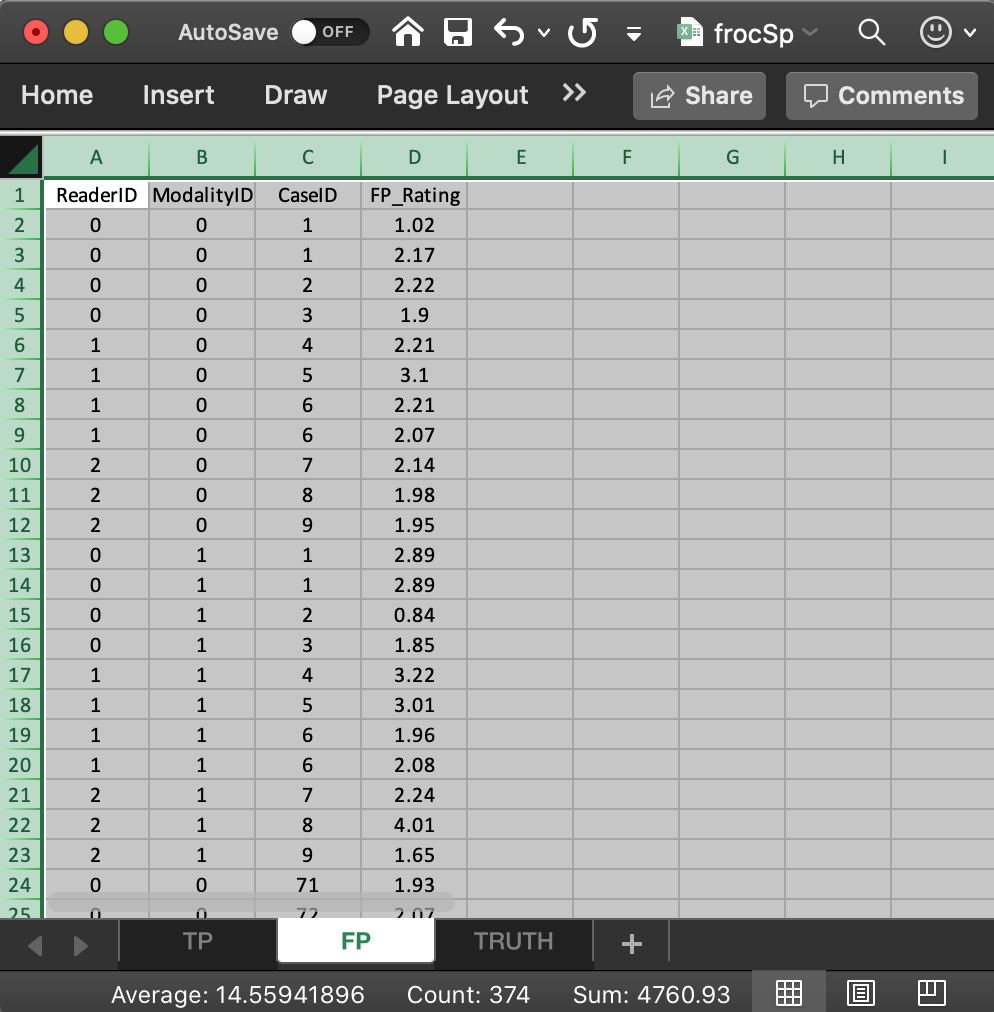
\includegraphics[width=0.5\linewidth,height=0.2\textheight]{images/frocSpNL} 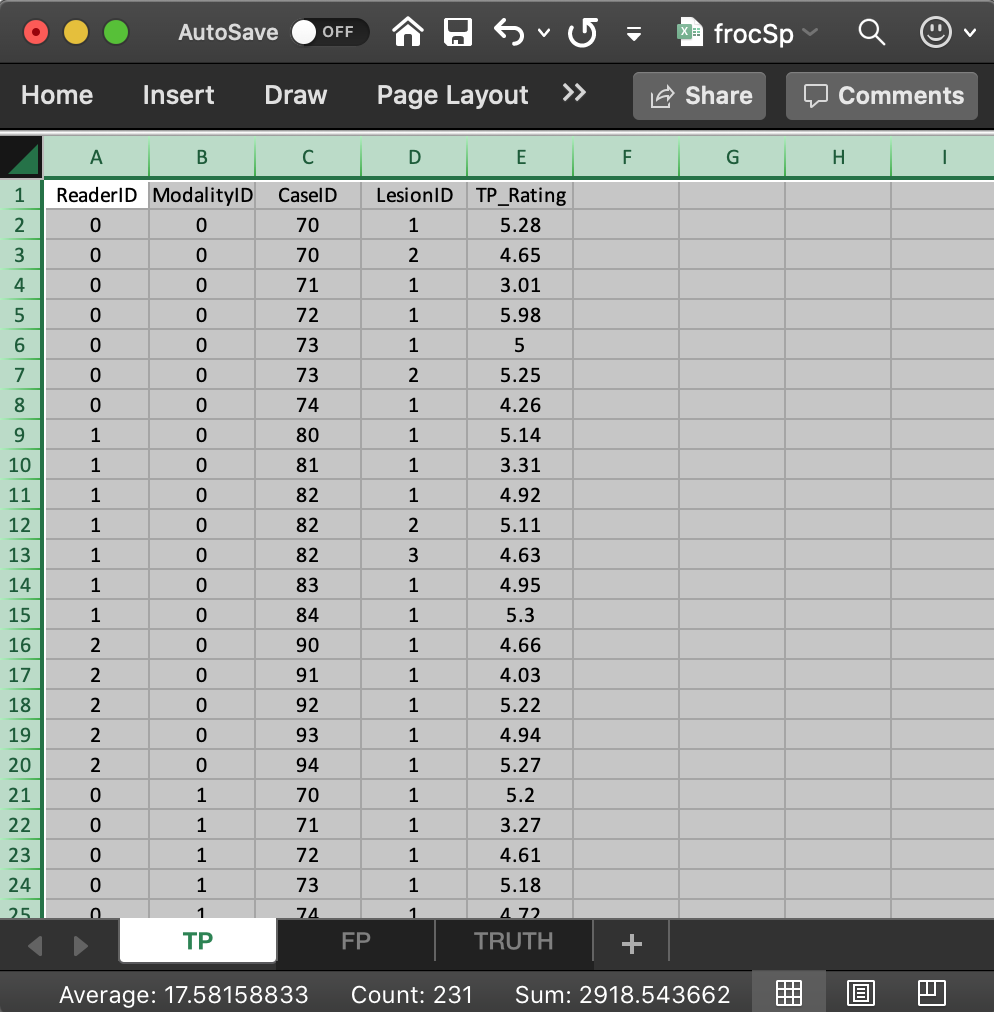
\includegraphics[width=0.5\linewidth,height=0.2\textheight]{images/frocSpLL} 

}

\caption{NL/FP worksheet, left, and LL/TP worksheet, right, for file frocSp.xlsx}\label{fig:frocSpLL}
\end{figure}

\begin{itemize}
\tightlist
\item
  This worksheet has the ratings of non-diseased cases.
\item
  The common vertical length is 30 in this example (2 modalities times 3 readers times 5 non-diseased cases per reader).
\item
  \texttt{ReaderID}: the reader labels: these must be from \texttt{0}, \texttt{1} or \texttt{2}, as declared in the \texttt{Truth} worksheet.
\item
  \texttt{ModalityID}: the modality labels: \texttt{0} or \texttt{1}, as declared in the \texttt{Truth} worksheet.
\item
  \texttt{CaseID}: the labels of non-diseased cases. Each \texttt{CaseID}, \texttt{ModalityID}, \texttt{ReaderID} combination must be consistent with that declared in the \texttt{Truth} worsheet.\\
\item
  \texttt{FP\_Rating}: the floating point ratings of non-diseased cases. Each row of this worksheet yields a rating corresponding to the values of \texttt{ReaderID}, \texttt{ModalityID} and \texttt{CaseID} for that row. Each \texttt{CaseID}, \texttt{ModalityID}, \texttt{ReaderID} combination must be consistent with that declared in the \texttt{Truth} worsheet.
\end{itemize}

\begin{Shaded}
\begin{Highlighting}[]
\NormalTok{x}\OperatorTok{$}\NormalTok{NL[,}\DecValTok{1}\NormalTok{,}\DecValTok{1}\OperatorTok{:}\DecValTok{9}\NormalTok{,}\DecValTok{1}\NormalTok{]}
\CommentTok{#>      [,1] [,2] [,3] [,4] [,5] [,6] [,7] [,8] [,9]}
\CommentTok{#> [1,] 1.02 2.22 1.90 -Inf -Inf -Inf -Inf -Inf -Inf}
\CommentTok{#> [2,] 2.89 0.84 1.85 -Inf -Inf -Inf -Inf -Inf -Inf}
\NormalTok{x}\OperatorTok{$}\NormalTok{NL[,}\DecValTok{2}\NormalTok{,}\DecValTok{1}\OperatorTok{:}\DecValTok{9}\NormalTok{,}\DecValTok{1}\NormalTok{]}
\CommentTok{#>      [,1] [,2] [,3] [,4] [,5] [,6] [,7] [,8] [,9]}
\CommentTok{#> [1,] -Inf -Inf -Inf 2.21 3.10 2.21 -Inf -Inf -Inf}
\CommentTok{#> [2,] -Inf -Inf -Inf 3.22 3.01 1.96 -Inf -Inf -Inf}
\NormalTok{x}\OperatorTok{$}\NormalTok{NL[,}\DecValTok{3}\NormalTok{,}\DecValTok{1}\OperatorTok{:}\DecValTok{9}\NormalTok{,}\DecValTok{1}\NormalTok{]}
\CommentTok{#>      [,1] [,2] [,3] [,4] [,5] [,6] [,7] [,8] [,9]}
\CommentTok{#> [1,] -Inf -Inf -Inf -Inf -Inf -Inf 2.14 1.98 1.95}
\CommentTok{#> [2,] -Inf -Inf -Inf -Inf -Inf -Inf 2.24 4.01 1.65}
\end{Highlighting}
\end{Shaded}

\begin{itemize}
\tightlist
\item
  The first line of the above code shows the ratings, in both modalities, of the first three non-diseased cases with \texttt{CaseID}s \texttt{1,3,3} (indexed 1, 2, 3 and appearing in the first three columns) interpreted by the first reader (\texttt{ReaderID} \texttt{0}).
\item
  The second line shows the ratings, in both modalities, of the next three non-diseased cases with \texttt{CaseID}s \texttt{4,5,6} (indexed 4, 5, 6and appearing in the next three columns) interpreted by the second reader (\texttt{ReaderID} \texttt{1}).
\item
  The third line shows the ratings, in both modalities, of the final three non-diseased cases with \texttt{CaseID}s \texttt{7,8,9} (indexed 7, 8, 9and appearing in the final three columns) interpreted by the third reader (\texttt{ReaderID} \texttt{2}).
\item
  Values such as \texttt{x\$NL{[},,16:30,1{]}}, which are there for compatibility with FROC data, are all filled with \texttt{-Inf}.
\end{itemize}

\hypertarget{the-true-positive-tp-ratings-3}{%
\section{The true positive (TP) ratings}\label{the-true-positive-tp-ratings-3}}

These are found in the \texttt{TP} or \texttt{LL} worksheet, see below.

\begin{itemize}
\tightlist
\item
  This worksheet has the ratings of diseased cases.
\item
  The common vertical length is 30 in this example (2 modalities times 3 readers times 5 diseased cases per reader).
\item
  \texttt{ReaderID}: the reader labels: these must be from \texttt{0}, \texttt{1} or \texttt{2}, as declared in the \texttt{Truth} worksheet.
\item
  \texttt{ModalityID}: the modality labels: \texttt{0} or \texttt{1}, as declared in the \texttt{Truth} worksheet.
\item
  \texttt{CaseID}: the labels of diseased cases. Each \texttt{CaseID}, \texttt{ModalityID}, \texttt{ReaderID} combination must be consistent with that declared in the \texttt{Truth} worsheet.\\
\item
  \texttt{TP\_Rating}: the floating point ratings of diseased cases. Each row of this worksheet yields a rating corresponding to the values of \texttt{ReaderID}, \texttt{ModalityID} and \texttt{CaseID} for that row. Each \texttt{CaseID}, \texttt{ModalityID}, \texttt{ReaderID} combination must be consistent with that declared in the \texttt{Truth} worsheet.
\end{itemize}

\begin{Shaded}
\begin{Highlighting}[]
\NormalTok{x}\OperatorTok{$}\NormalTok{LL[,}\DecValTok{1}\NormalTok{,}\DecValTok{1}\OperatorTok{:}\DecValTok{15}\NormalTok{,}\DecValTok{1}\NormalTok{]}
\CommentTok{#>      [,1] [,2] [,3] [,4] [,5] [,6] [,7] [,8] [,9] [,10] [,11] [,12] [,13] [,14]}
\CommentTok{#> [1,] 5.28 3.01 5.98 5.00 4.26 -Inf -Inf -Inf -Inf  -Inf  -Inf  -Inf  -Inf  -Inf}
\CommentTok{#> [2,] 5.20 3.27 4.61 5.18 4.72 -Inf -Inf -Inf -Inf  -Inf  -Inf  -Inf  -Inf  -Inf}
\CommentTok{#>      [,15]}
\CommentTok{#> [1,]  -Inf}
\CommentTok{#> [2,]  -Inf}
\NormalTok{x}\OperatorTok{$}\NormalTok{LL[,}\DecValTok{2}\NormalTok{,}\DecValTok{1}\OperatorTok{:}\DecValTok{15}\NormalTok{,}\DecValTok{1}\NormalTok{]}
\CommentTok{#>      [,1] [,2] [,3] [,4] [,5] [,6] [,7] [,8] [,9] [,10] [,11] [,12] [,13] [,14]}
\CommentTok{#> [1,] -Inf -Inf -Inf -Inf -Inf 5.14 3.31 4.92 4.95  5.30  -Inf  -Inf  -Inf  -Inf}
\CommentTok{#> [2,] -Inf -Inf -Inf -Inf -Inf 4.77 3.19 5.20 5.39  5.01  -Inf  -Inf  -Inf  -Inf}
\CommentTok{#>      [,15]}
\CommentTok{#> [1,]  -Inf}
\CommentTok{#> [2,]  -Inf}
\NormalTok{x}\OperatorTok{$}\NormalTok{LL[,}\DecValTok{3}\NormalTok{,}\DecValTok{1}\OperatorTok{:}\DecValTok{15}\NormalTok{,}\DecValTok{1}\NormalTok{]}
\CommentTok{#>      [,1] [,2] [,3] [,4] [,5] [,6] [,7] [,8] [,9] [,10] [,11] [,12] [,13] [,14]}
\CommentTok{#> [1,] -Inf -Inf -Inf -Inf -Inf -Inf -Inf -Inf -Inf  -Inf  4.66  4.03  5.22  4.94}
\CommentTok{#> [2,] -Inf -Inf -Inf -Inf -Inf -Inf -Inf -Inf -Inf  -Inf  4.87  1.94  -Inf  -Inf}
\CommentTok{#>      [,15]}
\CommentTok{#> [1,]  5.27}
\CommentTok{#> [2,]  4.78}
\end{Highlighting}
\end{Shaded}

\begin{itemize}
\tightlist
\item
  The first line of code shows the ratings, in both modalities, of the first five diseased cases with \texttt{CaseID}s \texttt{70,71,72,73,74} (indexed 1, 2, 3, 4, 5 and appearing in the first five columns) interpreted by the first reader (\texttt{ReaderID} \texttt{0}).
\item
  The second line shows the ratings, in both modalities, of the next five diseased cases with \texttt{CaseID}s \texttt{80,81,82,83,84} (indexed 6, 7, 8, 9, 10 and appearing in the next five columns) interpreted by the second reader (\texttt{ReaderID} \texttt{1}).
\item
  The third line shows the ratings, in both modalities, of the final five non-diseased cases with \texttt{CaseID}s \texttt{90,91,92,93,94} (indexed 11, 12, 13, 14, 15 and appearing in the final five columns) interpreted by the third reader (\texttt{ReaderID} \texttt{2}).
\end{itemize}

\hypertarget{summary-2}{%
\section{Summary}\label{summary-2}}

\begin{itemize}
\tightlist
\item
  TBA
\end{itemize}

\hypertarget{references-4}{%
\section{References}\label{references-4}}

\hypertarget{part-quick-start}{%
\part*{QUICK START}\label{part-quick-start}}
\addcontentsline{toc}{part}{QUICK START}

\hypertarget{QuickStartDBM1}{%
\chapter{QUICK START DBM1}\label{QuickStartDBM1}}

\hypertarget{introduction-4}{%
\section{Introduction}\label{introduction-4}}

\begin{itemize}
\tightlist
\item
  This vignette is intended for those seeking a quick transition from Windows \textbf{JAFROC} to \texttt{RJafroc}.
\item
  Described first is the structure of an \texttt{RJafroc} dataset followed by how to read
  a \emph{JAFROC} format Excel file to create an \texttt{RJafroc} dataset.
\end{itemize}

\hypertarget{an-roc-dataset}{%
\section{An ROC dataset}\label{an-roc-dataset}}

Dataset \texttt{dataset03} corresponding to the Franken ROC data \citep{RN1995} is predefined. The following code shows the structure of this dataset.

\begin{Shaded}
\begin{Highlighting}[]
\KeywordTok{str}\NormalTok{(dataset03)}
\CommentTok{#> List of 12}
\CommentTok{#>  $ NL           : num [1:2, 1:4, 1:100, 1] 3 3 4 3 3 3 4 1 1 3 ...}
\CommentTok{#>  $ LL           : num [1:2, 1:4, 1:67, 1] 5 5 4 4 5 4 4 5 2 2 ...}
\CommentTok{#>  $ lesionVector : num [1:67] 1 1 1 1 1 1 1 1 1 1 ...}
\CommentTok{#>  $ lesionID     : num [1:67, 1] 1 1 1 1 1 1 1 1 1 1 ...}
\CommentTok{#>  $ lesionWeight : num [1:67, 1] 1 1 1 1 1 1 1 1 1 1 ...}
\CommentTok{#>  $ dataType     : chr "ROC"}
\CommentTok{#>  $ modalityID   : Named chr [1:2] "TREAT1" "TREAT2"}
\CommentTok{#>   ..- attr(*, "names")= chr [1:2] "TREAT1" "TREAT2"}
\CommentTok{#>  $ readerID     : Named chr [1:4] "READER_1" "READER_2" "READER_3" "READER_4"}
\CommentTok{#>   ..- attr(*, "names")= chr [1:4] "READER_1" "READER_2" "READER_3" "READER_4"}
\CommentTok{#>  $ design       : chr "CROSSED"}
\CommentTok{#>  $ normalCases  : int [1:33] 1 2 3 4 5 6 7 8 9 10 ...}
\CommentTok{#>  $ abnormalCases: int [1:67] 34 35 36 37 38 39 40 41 42 43 ...}
\CommentTok{#>  $ truthTableStr: num [1:2, 1:4, 1:100, 1:2] 1 1 1 1 1 1 1 1 1 1 ...}
\end{Highlighting}
\end{Shaded}

\begin{itemize}
\item
  It is a list with 8 members. The false positive ratings are contained in \texttt{\{NL\}}, an array
  with dimensions \texttt{{[}1:2,1:4,1:100,1{]}}. The first index corresponds to treatments, and since the
  dataset has 2 treatments, the corresponding dimension is 2. The second index corresponds to
  readers, and since the dataset has 4 readers, the corresponding dimension is 4. The third index
  corresponds to the total number of cases. Since the dataset has 100 cases, the corresponding
  dimension is 100. But, as you can see from the code below, the entries in this array for cases 34
  through 100 are \texttt{-Inf}: i.e., \texttt{all(dataset03\$NL{[}1,1,34:100,1{]}\ ==\ -Inf)} = TRUE.
\item
  This is because in the ROC paradigm false positive are not possible on diseased cases. So the actual FP ratings are contained in the first 33 elements of the array. How did I know that there are 33 non-diseased cases? This can be understood in several ways.
\item
  \texttt{LL} is an array with dimensions \texttt{{[}1:2,1:4,1:67,1{]}}. This implies 67 diseased cases, and by subtraction from 100, there must be 33 non-diseased cases.
\item
  The list member \texttt{lesionVector} is a vector with length 67, implying 33 non-diseased cases.
\item
  The list members \texttt{lesionID} and \texttt{lesionWeight} are arrays with dimensions \texttt{{[}1:67,1{]}} containing ones. Again, these imply 67 diseased cases.
\item
  The fields \texttt{lesionVector}, \texttt{lesionID} and \texttt{lesionWeight}, while not needed for ROC data, are needed for the FROC paradigm.
\end{itemize}

The \texttt{dataType} list member is the character string \texttt{"ROC"}, characterizing the ROC dataset.

\begin{Shaded}
\begin{Highlighting}[]
\NormalTok{dataset03}\OperatorTok{$}\NormalTok{dataType}
\CommentTok{#> [1] "ROC"}
\end{Highlighting}
\end{Shaded}

The \texttt{modalityID} list member is a character string with two entries, \texttt{"TREAT1"} and \texttt{"TREAT2"}, corresponding to the two modalities.

\begin{Shaded}
\begin{Highlighting}[]
\NormalTok{dataset03}\OperatorTok{$}\NormalTok{modalityID}
\CommentTok{#>   TREAT1   TREAT2 }
\CommentTok{#> "TREAT1" "TREAT2"}
\end{Highlighting}
\end{Shaded}

The \texttt{readerID} list member is a character string with four entries, \texttt{"READER\_1"}, \texttt{"READER\_2"}, \texttt{"READER\_3"} and \texttt{"READER\_4"} corresponding to the four readers.

\begin{Shaded}
\begin{Highlighting}[]
\NormalTok{dataset03}\OperatorTok{$}\NormalTok{readerID}
\CommentTok{#>   READER_1   READER_2   READER_3   READER_4 }
\CommentTok{#> "READER_1" "READER_2" "READER_3" "READER_4"}
\end{Highlighting}
\end{Shaded}

Here are the actual ratings for cases 1:34.

\begin{Shaded}
\begin{Highlighting}[]
\NormalTok{dataset03}\OperatorTok{$}\NormalTok{NL[}\DecValTok{1}\NormalTok{,}\DecValTok{1}\NormalTok{,}\DecValTok{1}\OperatorTok{:}\DecValTok{33}\NormalTok{,}\DecValTok{1}\NormalTok{]}
\CommentTok{#>  [1] 3 1 2 2 2 2 2 4 1 1 4 2 1 2 4 2 1 2 1 2 4 2 3 2 2 2 4 3 2 2 2 5 3}
\end{Highlighting}
\end{Shaded}

\begin{itemize}
\item
  This says that for treatment 1 and reader 1, (non-diseased) case 1 was rated 3, case 2 was rated 1, cases 3-7 were rated 2, case 8 was rated 4, etc.
\item
  As another example, for treatment 2 and reader 3, the FP ratings are:
\end{itemize}

\begin{Shaded}
\begin{Highlighting}[]
\NormalTok{dataset03}\OperatorTok{$}\NormalTok{NL[}\DecValTok{2}\NormalTok{,}\DecValTok{3}\NormalTok{,}\DecValTok{1}\OperatorTok{:}\DecValTok{33}\NormalTok{,}\DecValTok{1}\NormalTok{]}
\CommentTok{#>  [1] 3 1 2 2 2 2 4 4 2 3 2 2 1 3 2 4 2 3 2 2 2 2 2 4 2 2 1 2 2 2 2 4 2}
\end{Highlighting}
\end{Shaded}

\hypertarget{creating-a-dataset-from-a-jafroc-format-file}{%
\section{Creating a dataset from a JAFROC format file}\label{creating-a-dataset-from-a-jafroc-format-file}}

There is a file \texttt{RocData.xlsx} that is part of the package installation. Since it is a system
file one must get its name as follows.

\begin{Shaded}
\begin{Highlighting}[]
\NormalTok{fileName <-}\StringTok{ "RocData.xlsx"}
\NormalTok{sysFileName <-}\StringTok{ }\KeywordTok{system.file}\NormalTok{(}\KeywordTok{paste0}\NormalTok{(}\StringTok{"extdata/"}\NormalTok{,fileName), }\DataTypeTok{package =} \StringTok{"RJafroc"}\NormalTok{, }\DataTypeTok{mustWork =} \OtherTok{TRUE}\NormalTok{)}
\end{Highlighting}
\end{Shaded}

Next, one uses \texttt{DfReadDataFile()} as follows, assuming it is a JAFROC format file.

\begin{Shaded}
\begin{Highlighting}[]
\NormalTok{ds <-}\StringTok{ }\KeywordTok{DfReadDataFile}\NormalTok{(sysFileName, }\DataTypeTok{newExcelFileFormat =} \OtherTok{FALSE}\NormalTok{)}
\KeywordTok{str}\NormalTok{(ds)}
\CommentTok{#> List of 12}
\CommentTok{#>  $ NL           : num [1:2, 1:5, 1:114, 1] 1 3 2 3 2 2 1 2 3 2 ...}
\CommentTok{#>  $ LL           : num [1:2, 1:5, 1:45, 1] 5 5 5 5 5 5 5 5 5 5 ...}
\CommentTok{#>  $ lesionVector : int [1:45] 1 1 1 1 1 1 1 1 1 1 ...}
\CommentTok{#>  $ lesionID     : num [1:45, 1] 1 1 1 1 1 1 1 1 1 1 ...}
\CommentTok{#>  $ lesionWeight : num [1:45, 1] 1 1 1 1 1 1 1 1 1 1 ...}
\CommentTok{#>  $ dataType     : chr "ROC"}
\CommentTok{#>  $ modalityID   : Named chr [1:2] "0" "1"}
\CommentTok{#>   ..- attr(*, "names")= chr [1:2] "0" "1"}
\CommentTok{#>  $ readerID     : Named chr [1:5] "0" "1" "2" "3" ...}
\CommentTok{#>   ..- attr(*, "names")= chr [1:5] "0" "1" "2" "3" ...}
\CommentTok{#>  $ design       : chr "CROSSED"}
\CommentTok{#>  $ normalCases  : int [1:69] 1 2 3 4 5 6 7 8 9 10 ...}
\CommentTok{#>  $ abnormalCases: int [1:45] 70 71 72 73 74 75 76 77 78 79 ...}
\CommentTok{#>  $ truthTableStr: num [1:2, 1:5, 1:114, 1:2] 1 1 1 1 1 1 1 1 1 1 ...}
\end{Highlighting}
\end{Shaded}

Analysis is illustrated for \texttt{dataset03}, but one could have used the newly created dataset \texttt{ds}.

\hypertarget{analyzing-the-roc-dataset}{%
\section{Analyzing the ROC dataset}\label{analyzing-the-roc-dataset}}

This illustrates the \texttt{StSignificanceTesting()} function. The significance testing method is specified as \texttt{"DBMH"} and the figure of merit \texttt{FOM} is specified as ``Wilcoxon''.

\begin{Shaded}
\begin{Highlighting}[]
\NormalTok{ret <-}\StringTok{ }\KeywordTok{StSignificanceTesting}\NormalTok{(dataset03, }\DataTypeTok{FOM =} \StringTok{"Wilcoxon"}\NormalTok{, }\DataTypeTok{method =} \StringTok{"DBMH"}\NormalTok{)}
\KeywordTok{print}\NormalTok{(ret)}
\CommentTok{#> $fomArray}
\CommentTok{#>           RdrREADER_1 RdrREADER_2 RdrREADER_3 RdrREADER_4}
\CommentTok{#> TrtTREAT1   0.8534600   0.8649932   0.8573044   0.8152420}
\CommentTok{#> TrtTREAT2   0.8496156   0.8435097   0.8401176   0.8143374}
\CommentTok{#> }
\CommentTok{#> $anovaY}
\CommentTok{#>       Source           SS  DF          MS}
\CommentTok{#> 1     Row1_T   0.02356541   1 0.023565410}
\CommentTok{#> 2     Row2_R   0.20521800   3 0.068406000}
\CommentTok{#> 3     Row3_C  52.52839868  99 0.530589886}
\CommentTok{#> 4    Row4_TR   0.01506079   3 0.005020264}
\CommentTok{#> 5    Row5_TC   6.41004881  99 0.064747968}
\CommentTok{#> 6    Row6_RC  39.24295381 297 0.132131158}
\CommentTok{#> 7   Row7_TRC  22.66007764 297 0.076296558}
\CommentTok{#> 8 Row8_Total 121.08532315 799          NA}
\CommentTok{#> }
\CommentTok{#> $anovaYi}
\CommentTok{#>   Source  DF  TrtTREAT1  TrtTREAT2}
\CommentTok{#> 1      R   3 0.04926635 0.02415991}
\CommentTok{#> 2      C  99 0.29396753 0.30137032}
\CommentTok{#> 3     RC 297 0.10504787 0.10337984}
\CommentTok{#> }
\CommentTok{#> $varComp}
\CommentTok{#>           varR       varC         varTR        varTC     varRC     varErr}
\CommentTok{#> 1 3.775568e-05 0.05125091 -0.0007127629 -0.002887147 0.0279173 0.07629656}
\CommentTok{#> }
\CommentTok{#> $FTestStatsRRRC}
\CommentTok{#>      fRRRC ndfRRRC ddfRRRC     pRRRC}
\CommentTok{#> 1 4.694058       1       3 0.1188379}
\CommentTok{#> }
\CommentTok{#> $ciDiffTrtRRRC}
\CommentTok{#>               TrtDiff   Estimate      StdErr DF        t     PrGTt      CILower}
\CommentTok{#> 1 TrtTREAT1-TrtTREAT2 0.01085482 0.005010122  3 2.166577 0.1188379 -0.005089627}
\CommentTok{#>      CIUpper}
\CommentTok{#> 1 0.02679926}
\CommentTok{#> }
\CommentTok{#> $ciAvgRdrEachTrtRRRC}
\CommentTok{#>   Treatment      Area     StdErr        DF   CILower   CIUpper}
\CommentTok{#> 1 TrtTREAT1 0.8477499 0.02440215  70.12179 0.7990828 0.8964170}
\CommentTok{#> 2 TrtTREAT2 0.8368951 0.02356642 253.64403 0.7904843 0.8833058}
\CommentTok{#> }
\CommentTok{#> $FTestStatsFRRC}
\CommentTok{#>      fFRRC ndfFRRC ddfFRRC    pFRRC}
\CommentTok{#> 1 0.363956       1      99 0.547697}
\CommentTok{#> }
\CommentTok{#> $ciDiffTrtFRRC}
\CommentTok{#>             Treatment   Estimate     StdErr DF         t    PrGTt     CILower}
\CommentTok{#> 1 TrtTREAT1-TrtTREAT2 0.01085482 0.01799277 99 0.6032876 0.547697 -0.02484675}
\CommentTok{#>      CIUpper}
\CommentTok{#> 1 0.04655638}
\CommentTok{#> }
\CommentTok{#> $ciAvgRdrEachTrtFRRC}
\CommentTok{#>   Treatment      Area     StdErr DF   CILower   CIUpper}
\CommentTok{#> 1 TrtTREAT1 0.8477499 0.02710939 99 0.7939590 0.9015408}
\CommentTok{#> 2 TrtTREAT2 0.8368951 0.02744860 99 0.7824311 0.8913591}
\CommentTok{#> }
\CommentTok{#> $msAnovaEachRdrFRRC}
\CommentTok{#>   Source DF  RdrREADER_1 RdrREADER_2 RdrREADER_3  RdrREADER_4}
\CommentTok{#> 1      T  1 0.0007389761  0.02307702  0.01476929 4.091217e-05}
\CommentTok{#> 2      C 99 0.2038747746  0.22344191  0.21424677 2.854199e-01}
\CommentTok{#> 3     TC 99 0.0915587344  0.08027926  0.06122898 6.057067e-02}
\CommentTok{#> }
\CommentTok{#> $ciDiffTrtEachRdrFRRC}
\CommentTok{#>        Reader           Treatment     Estimate     StdErr DF          t}
\CommentTok{#> 1 RdrREADER_1 TrtTREAT1-TrtTREAT2 0.0038444143 0.04279223 99 0.08983908}
\CommentTok{#> 2 RdrREADER_2 TrtTREAT1-TrtTREAT2 0.0214834916 0.04006975 99 0.53615233}
\CommentTok{#> 3 RdrREADER_3 TrtTREAT1-TrtTREAT2 0.0171867933 0.03499399 99 0.49113552}
\CommentTok{#> 4 RdrREADER_4 TrtTREAT1-TrtTREAT2 0.0009045681 0.03480536 99 0.02598933}
\CommentTok{#>       PrGTt     CILower    CIUpper}
\CommentTok{#> 1 0.9285966 -0.08106465 0.08875348}
\CommentTok{#> 2 0.5930559 -0.05802359 0.10099057}
\CommentTok{#> 3 0.6244176 -0.05224888 0.08662247}
\CommentTok{#> 4 0.9793182 -0.06815683 0.06996596}
\CommentTok{#> }
\CommentTok{#> $FTestStatsRRFC}
\CommentTok{#>      fRRFC ndfRRFC ddfRRFC     pRRFC}
\CommentTok{#> 1 4.694058       1       3 0.1188379}
\CommentTok{#> }
\CommentTok{#> $ciDiffTrtRRFC}
\CommentTok{#>             Treatment   Estimate      StdErr DF        t     PrGTt      CILower}
\CommentTok{#> 1 TrtTREAT1-TrtTREAT2 0.01085482 0.005010122  3 2.166577 0.1188379 -0.005089627}
\CommentTok{#>      CIUpper}
\CommentTok{#> 1 0.02679926}
\CommentTok{#> }
\CommentTok{#> $ciAvgRdrEachTrtRRFC}
\CommentTok{#>   Treatment      Area     StdErr DF   CILower   CIUpper}
\CommentTok{#> 1 TrtTREAT1 0.8477499 0.01109801  3 0.8124311 0.8830687}
\CommentTok{#> 2 TrtTREAT2 0.8368951 0.00777173  3 0.8121620 0.8616282}
\end{Highlighting}
\end{Shaded}

\hypertarget{explanation-of-the-output}{%
\section{Explanation of the output}\label{explanation-of-the-output}}

The function returns a long unwieldy list. Let us consider them one by one. The function \texttt{UtilOutputReport()}, which can generate an Excel file report, making it much easier to visualize the results, is described in another vignette.

\hypertarget{foms}{%
\subsection{FOMs}\label{foms}}

\begin{itemize}
\tightlist
\item
  \texttt{fomArray} contains the \texttt{{[}1:2,1:4{]}} FOM values.
\end{itemize}

\begin{Shaded}
\begin{Highlighting}[]
\NormalTok{ret}\OperatorTok{$}\NormalTok{fomArray}
\CommentTok{#>           RdrREADER_1 RdrREADER_2 RdrREADER_3 RdrREADER_4}
\CommentTok{#> TrtTREAT1   0.8534600   0.8649932   0.8573044   0.8152420}
\CommentTok{#> TrtTREAT2   0.8496156   0.8435097   0.8401176   0.8143374}
\end{Highlighting}
\end{Shaded}

This shows the 2 x 4 array of FOM values.

\hypertarget{pseudovalue-anova-table}{%
\subsection{Pseudovalue ANOVA table}\label{pseudovalue-anova-table}}

\begin{itemize}
\tightlist
\item
  \texttt{anovaY}, where the Y denotes that these are pseudovalue based, is the ANOVA table.
\end{itemize}

\begin{Shaded}
\begin{Highlighting}[]
\NormalTok{ret}\OperatorTok{$}\NormalTok{anovaY}
\CommentTok{#>       Source           SS  DF          MS}
\CommentTok{#> 1     Row1_T   0.02356541   1 0.023565410}
\CommentTok{#> 2     Row2_R   0.20521800   3 0.068406000}
\CommentTok{#> 3     Row3_C  52.52839868  99 0.530589886}
\CommentTok{#> 4    Row4_TR   0.01506079   3 0.005020264}
\CommentTok{#> 5    Row5_TC   6.41004881  99 0.064747968}
\CommentTok{#> 6    Row6_RC  39.24295381 297 0.132131158}
\CommentTok{#> 7   Row7_TRC  22.66007764 297 0.076296558}
\CommentTok{#> 8 Row8_Total 121.08532315 799          NA}
\end{Highlighting}
\end{Shaded}

\hypertarget{pseudovalue-anova-table-each-treatment}{%
\subsection{Pseudovalue ANOVA table, each treatment}\label{pseudovalue-anova-table-each-treatment}}

\begin{itemize}
\tightlist
\item
  \texttt{anovaYi} is the ANOVA table for individual treatments.
\end{itemize}

\begin{Shaded}
\begin{Highlighting}[]
\NormalTok{ret}\OperatorTok{$}\NormalTok{anovaYi}
\CommentTok{#>   Source  DF  TrtTREAT1  TrtTREAT2}
\CommentTok{#> 1      R   3 0.04926635 0.02415991}
\CommentTok{#> 2      C  99 0.29396753 0.30137032}
\CommentTok{#> 3     RC 297 0.10504787 0.10337984}
\end{Highlighting}
\end{Shaded}

The \texttt{0} and \texttt{1} headers come from the treatment names.

\hypertarget{pseudovalue-variance-components}{%
\subsection{Pseudovalue Variance Components}\label{pseudovalue-variance-components}}

\begin{itemize}
\tightlist
\item
  \texttt{varComp} is the variance components (needed for sample size estimation).
\end{itemize}

\begin{Shaded}
\begin{Highlighting}[]
\NormalTok{ret}\OperatorTok{$}\NormalTok{varComp}
\CommentTok{#>           varR       varC         varTR        varTC     varRC     varErr}
\CommentTok{#> 1 3.775568e-05 0.05125091 -0.0007127629 -0.002887147 0.0279173 0.07629656}
\end{Highlighting}
\end{Shaded}

\hypertarget{random-reader-random-case-rrrc-analysis}{%
\subsection{Random-reader random-case (RRRC) analysis}\label{random-reader-random-case-rrrc-analysis}}

\begin{itemize}
\tightlist
\item
  \texttt{ret\$FTestStatsRRRC\$fRRRC} is the F-statistic for testing the NH that the
  treatments have identical FOMs. RRRC means random-reader random-case generalization.
\end{itemize}

\begin{Shaded}
\begin{Highlighting}[]
\NormalTok{ret}\OperatorTok{$}\NormalTok{FTestStatsRRRC}\OperatorTok{$}\NormalTok{fRRRC}
\CommentTok{#> [1] 4.694058}
\end{Highlighting}
\end{Shaded}

\hypertarget{f-statistic-and-p-value-for-rrrc-analysis}{%
\subsubsection{F-statistic and p-value for RRRC analysis}\label{f-statistic-and-p-value-for-rrrc-analysis}}

\begin{itemize}
\tightlist
\item
  \texttt{ret\$FTestStatsRRRC\$ddfRRRC} is the denominator degrees of freedom of the F-statistic.
\end{itemize}

\begin{Shaded}
\begin{Highlighting}[]
\NormalTok{ret}\OperatorTok{$}\NormalTok{FTestStatsRRRC}\OperatorTok{$}\NormalTok{ddfRRRC}
\CommentTok{#> [1] 3}
\end{Highlighting}
\end{Shaded}

\begin{itemize}
\tightlist
\item
  \texttt{ret\$FTestStatsRRRC\$pRRRC} is the p-value of the test.
\end{itemize}

\begin{Shaded}
\begin{Highlighting}[]
\NormalTok{ret}\OperatorTok{$}\NormalTok{FTestStatsRRRC}\OperatorTok{$}\NormalTok{pRRRC}
\CommentTok{#> [1] 0.1188379}
\end{Highlighting}
\end{Shaded}

\hypertarget{confidence-intervals-for-rrrc-analysis}{%
\subsubsection{Confidence Intervals for RRRC analysis}\label{confidence-intervals-for-rrrc-analysis}}

\begin{itemize}
\tightlist
\item
  \texttt{ciDiffTrtRRRC} is the 95\% confidence interval of reader-averaged differences between treatments.
\end{itemize}

\begin{Shaded}
\begin{Highlighting}[]
\NormalTok{ret}\OperatorTok{$}\NormalTok{ciDiffTrtRRRC}
\CommentTok{#>               TrtDiff   Estimate      StdErr DF        t     PrGTt      CILower}
\CommentTok{#> 1 TrtTREAT1-TrtTREAT2 0.01085482 0.005010122  3 2.166577 0.1188379 -0.005089627}
\CommentTok{#>      CIUpper}
\CommentTok{#> 1 0.02679926}
\end{Highlighting}
\end{Shaded}

\begin{itemize}
\tightlist
\item
  \texttt{ciAvgRdrEachTrtRRRC} is the 95\% confidence interval of reader-averaged FOMs for each treatments.
\end{itemize}

\begin{Shaded}
\begin{Highlighting}[]
\NormalTok{ret}\OperatorTok{$}\NormalTok{ciAvgRdrEachTrtRRRC}
\CommentTok{#>   Treatment      Area     StdErr        DF   CILower   CIUpper}
\CommentTok{#> 1 TrtTREAT1 0.8477499 0.02440215  70.12179 0.7990828 0.8964170}
\CommentTok{#> 2 TrtTREAT2 0.8368951 0.02356642 253.64403 0.7904843 0.8833058}
\end{Highlighting}
\end{Shaded}

\hypertarget{fixed-reader-random-case-frrc-analysis}{%
\subsection{Fixed-reader random-case (FRRC) analysis}\label{fixed-reader-random-case-frrc-analysis}}

\hypertarget{f-statistic-and-p-value-for-frrc-analysis}{%
\subsubsection{F-statistic and p-value for FRRC analysis}\label{f-statistic-and-p-value-for-frrc-analysis}}

\begin{itemize}
\tightlist
\item
  \texttt{ret\$FTestStatsFRRC\$fFRRC} is the F-statistic for fixed-reader random-case analysis.
\end{itemize}

\begin{Shaded}
\begin{Highlighting}[]
\NormalTok{ret}\OperatorTok{$}\NormalTok{FTestStatsFRRC}\OperatorTok{$}\NormalTok{fFRRC}
\CommentTok{#> [1] 0.363956}
\end{Highlighting}
\end{Shaded}

\begin{itemize}
\tightlist
\item
  \texttt{ret\$FTestStatsFRRC\$ndfFRRC} is the numerator degrees of freedom of the F-statistic, always one less than the number of treatments.
\end{itemize}

\begin{Shaded}
\begin{Highlighting}[]
\NormalTok{ret}\OperatorTok{$}\NormalTok{FTestStatsFRRC}\OperatorTok{$}\NormalTok{ndfFRRC}
\CommentTok{#> [1] 1}
\end{Highlighting}
\end{Shaded}

\begin{itemize}
\tightlist
\item
  \texttt{ret\$FTestStatsFRRC\$ddfFRRC} is the denominator degreesof freedom of the F-statistic, for fixed-reader random-case analysis.
\end{itemize}

\begin{Shaded}
\begin{Highlighting}[]
\NormalTok{ret}\OperatorTok{$}\NormalTok{FTestStatsFRRC}\OperatorTok{$}\NormalTok{ddfFRRC}
\CommentTok{#> [1] 99}
\end{Highlighting}
\end{Shaded}

\begin{itemize}
\tightlist
\item
  \texttt{ret\$FTestStatsFRRC\$pFRRC} is the p-value for fixed-reader random-case analysis.
\end{itemize}

\begin{Shaded}
\begin{Highlighting}[]
\NormalTok{ret}\OperatorTok{$}\NormalTok{FTestStatsFRRC}\OperatorTok{$}\NormalTok{pFRRC}
\CommentTok{#> [1] 0.547697}
\end{Highlighting}
\end{Shaded}

\hypertarget{confidence-intervals-for-frrc-analysis}{%
\subsubsection{Confidence Intervals for FRRC analysis}\label{confidence-intervals-for-frrc-analysis}}

\begin{itemize}
\tightlist
\item
  \texttt{ciDiffTrtFRRC} is the 95\% CI of reader-average differences between treatments for fixed-reader random-case analysis
\end{itemize}

\begin{Shaded}
\begin{Highlighting}[]
\NormalTok{ret}\OperatorTok{$}\NormalTok{ciDiffTrtFRRC}
\CommentTok{#>             Treatment   Estimate     StdErr DF         t    PrGTt     CILower}
\CommentTok{#> 1 TrtTREAT1-TrtTREAT2 0.01085482 0.01799277 99 0.6032876 0.547697 -0.02484675}
\CommentTok{#>      CIUpper}
\CommentTok{#> 1 0.04655638}
\end{Highlighting}
\end{Shaded}

\begin{itemize}
\tightlist
\item
  \texttt{ret\$ciAvgRdrEachTrtFRRC} is the 95\% CI of reader-average FOMs of each treatment for fixed-reader random-case analysis
\end{itemize}

\begin{Shaded}
\begin{Highlighting}[]
\NormalTok{ret}\OperatorTok{$}\NormalTok{ciAvgRdrEachTrtFRRC}
\CommentTok{#>   Treatment      Area     StdErr DF   CILower   CIUpper}
\CommentTok{#> 1 TrtTREAT1 0.8477499 0.02710939 99 0.7939590 0.9015408}
\CommentTok{#> 2 TrtTREAT2 0.8368951 0.02744860 99 0.7824311 0.8913591}
\end{Highlighting}
\end{Shaded}

\hypertarget{anova-for-frrc-analysis}{%
\subsubsection{ANOVA for FRRC analysis}\label{anova-for-frrc-analysis}}

\begin{itemize}
\tightlist
\item
  \texttt{ret\$msAnovaEachRdrFRRC} is the mean-squares ANOVA for each reader
\end{itemize}

\begin{Shaded}
\begin{Highlighting}[]
\NormalTok{ret}\OperatorTok{$}\NormalTok{msAnovaEachRdrFRRC}
\CommentTok{#>   Source DF  RdrREADER_1 RdrREADER_2 RdrREADER_3  RdrREADER_4}
\CommentTok{#> 1      T  1 0.0007389761  0.02307702  0.01476929 4.091217e-05}
\CommentTok{#> 2      C 99 0.2038747746  0.22344191  0.21424677 2.854199e-01}
\CommentTok{#> 3     TC 99 0.0915587344  0.08027926  0.06122898 6.057067e-02}
\end{Highlighting}
\end{Shaded}

\hypertarget{confidence-intervals-for-frrc-analysis-1}{%
\subsubsection{Confidence Intervals for FRRC analysis}\label{confidence-intervals-for-frrc-analysis-1}}

\begin{itemize}
\tightlist
\item
  \texttt{ciDiffTrtFRRC} is the CI for reader-averaged treatment differences, for fixed-reader random-case analysis
\end{itemize}

\begin{Shaded}
\begin{Highlighting}[]
\NormalTok{ret}\OperatorTok{$}\NormalTok{ciDiffTrtFRRC}
\CommentTok{#>             Treatment   Estimate     StdErr DF         t    PrGTt     CILower}
\CommentTok{#> 1 TrtTREAT1-TrtTREAT2 0.01085482 0.01799277 99 0.6032876 0.547697 -0.02484675}
\CommentTok{#>      CIUpper}
\CommentTok{#> 1 0.04655638}
\end{Highlighting}
\end{Shaded}

\hypertarget{random-reader-fixed-case-rrfc-analysis}{%
\subsection{Random-reader fixed-case (RRFC) analysis}\label{random-reader-fixed-case-rrfc-analysis}}

\hypertarget{f-statistic-and-p-value-for-rrfc-analysis}{%
\subsubsection{F-statistic and p-value for RRFC analysis}\label{f-statistic-and-p-value-for-rrfc-analysis}}

\begin{itemize}
\tightlist
\item
  \texttt{ret\$FTestStatsRRFC\$fRRFC} is the F-statistic for for random-reader fixed-case analysis
\end{itemize}

\begin{Shaded}
\begin{Highlighting}[]
\NormalTok{ret}\OperatorTok{$}\NormalTok{FTestStatsRRFC}\OperatorTok{$}\NormalTok{fRRFC}
\CommentTok{#> [1] 4.694058}
\end{Highlighting}
\end{Shaded}

\begin{itemize}
\tightlist
\item
  \texttt{ret\$FTestStatsRRFC\$ddfRRFC} is the ddf for for random-reader fixed-case analysis
\end{itemize}

\begin{Shaded}
\begin{Highlighting}[]
\NormalTok{ret}\OperatorTok{$}\NormalTok{FTestStatsRRFC}\OperatorTok{$}\NormalTok{ddfRRFC}
\CommentTok{#> [1] 3}
\end{Highlighting}
\end{Shaded}

\begin{itemize}
\tightlist
\item
  \texttt{ret\$FTestStatsRRFC\$pRRFC} is the p-value for for random-reader fixed-case analysis
\end{itemize}

\begin{Shaded}
\begin{Highlighting}[]
\NormalTok{ret}\OperatorTok{$}\NormalTok{FTestStatsRRFC}\OperatorTok{$}\NormalTok{pRRFC}
\CommentTok{#> [1] 0.1188379}
\end{Highlighting}
\end{Shaded}

\hypertarget{confidence-intervals-for-rrfc-analysis}{%
\subsubsection{Confidence Intervals for RRFC analysis}\label{confidence-intervals-for-rrfc-analysis}}

\begin{itemize}
\tightlist
\item
  \texttt{ciDiffTrtRRFC} is the CI for reader-averaged inter-treatment FOM differences for random-reader fixed-case analysis
\end{itemize}

\begin{Shaded}
\begin{Highlighting}[]
\NormalTok{ret}\OperatorTok{$}\NormalTok{ciDiffTrtRRFC}
\CommentTok{#>             Treatment   Estimate      StdErr DF        t     PrGTt      CILower}
\CommentTok{#> 1 TrtTREAT1-TrtTREAT2 0.01085482 0.005010122  3 2.166577 0.1188379 -0.005089627}
\CommentTok{#>      CIUpper}
\CommentTok{#> 1 0.02679926}
\end{Highlighting}
\end{Shaded}

\begin{itemize}
\tightlist
\item
  \texttt{ciAvgRdrEachTrtRRFC} is the CI for treatment FOMs for each reader for random-reader fixed-case analysis
\end{itemize}

\begin{Shaded}
\begin{Highlighting}[]
\NormalTok{ret}\OperatorTok{$}\NormalTok{ciAvgRdrEachTrtRRFC}
\CommentTok{#>   Treatment      Area     StdErr DF   CILower   CIUpper}
\CommentTok{#> 1 TrtTREAT1 0.8477499 0.01109801  3 0.8124311 0.8830687}
\CommentTok{#> 2 TrtTREAT2 0.8368951 0.00777173  3 0.8121620 0.8616282}
\end{Highlighting}
\end{Shaded}

\hypertarget{orh-significance-testing}{%
\section{ORH significance testing}\label{orh-significance-testing}}

Simply change \texttt{method\ =\ "DBMH"} to \texttt{method\ =\ "ORH"}.

\begin{Shaded}
\begin{Highlighting}[]
\NormalTok{ret <-}\StringTok{ }\KeywordTok{StSignificanceTesting}\NormalTok{(dataset03, }\DataTypeTok{FOM =} \StringTok{"Wilcoxon"}\NormalTok{, }\DataTypeTok{method =} \StringTok{"ORH"}\NormalTok{)}
\KeywordTok{str}\NormalTok{(ret)}
\CommentTok{#> List of 14}
\CommentTok{#>  $ fomArray            : num [1:2, 1:4] 0.853 0.85 0.865 0.844 0.857 ...}
\CommentTok{#>   ..- attr(*, "dimnames")=List of 2}
\CommentTok{#>   .. ..$ : chr [1:2] "TrtTREAT1" "TrtTREAT2"}
\CommentTok{#>   .. ..$ : chr [1:4] "RdrREADER_1" "RdrREADER_2" "RdrREADER_3" "RdrREADER_4"}
\CommentTok{#>  $ meanSquares         :'data.frame':    1 obs. of  3 variables:}
\CommentTok{#>   ..$ msT : num 0.000236}
\CommentTok{#>   ..$ msR : num 0.000684}
\CommentTok{#>   ..$ msTR: num 5.02e-05}
\CommentTok{#>  $ varComp             :'data.frame':    1 obs. of  6 variables:}
\CommentTok{#>   ..$ varR : num 2.33e-05}
\CommentTok{#>   ..$ varTR: num -0.000684}
\CommentTok{#>   ..$ cov1 : num 0.000792}
\CommentTok{#>   ..$ cov2 : num 0.000484}
\CommentTok{#>   ..$ cov3 : num 0.000513}
\CommentTok{#>   ..$ var  : num 0.00153}
\CommentTok{#>  $ FTestStatsRRRC      :'data.frame':    1 obs. of  4 variables:}
\CommentTok{#>   ..$ fRRRC  : num 4.69}
\CommentTok{#>   ..$ ndfRRRC: num 1}
\CommentTok{#>   ..$ ddfRRRC: num 3}
\CommentTok{#>   ..$ pRRRC  : num 0.119}
\CommentTok{#>  $ ciDiffTrtRRRC       :'data.frame':    1 obs. of  8 variables:}
\CommentTok{#>   ..$ Treatment: chr "TrtTREAT1-TrtTREAT2"}
\CommentTok{#>   ..$ Estimate : num 0.0109}
\CommentTok{#>   ..$ StdErr   : num 0.00501}
\CommentTok{#>   ..$ DF       : num 3}
\CommentTok{#>   ..$ t        : num 2.17}
\CommentTok{#>   ..$ PrGTt    : num 0.119}
\CommentTok{#>   ..$ CILower  : num -0.00509}
\CommentTok{#>   ..$ CIUpper  : num 0.0268}
\CommentTok{#>  $ ciAvgRdrEachTrtRRRC :'data.frame':    2 obs. of  6 variables:}
\CommentTok{#>   ..$ Treatment: Factor w/ 2 levels "TrtTREAT1","TrtTREAT2": 1 2}
\CommentTok{#>   ..$ Area     : num [1:2] 0.848 0.837}
\CommentTok{#>   ..$ StdErr   : num [1:2] 0.0244 0.0236}
\CommentTok{#>   ..$ DF       : num [1:2] 70.1 253.6}
\CommentTok{#>   ..$ CILower  : num [1:2] 0.799 0.79}
\CommentTok{#>   ..$ CIUpper  : num [1:2] 0.896 0.883}
\CommentTok{#>  $ FTestStatsFRRC      :'data.frame':    1 obs. of  4 variables:}
\CommentTok{#>   ..$ fFRRC  : num 0.364}
\CommentTok{#>   ..$ ndfFRRC: num 1}
\CommentTok{#>   ..$ ddfFRRC: num Inf}
\CommentTok{#>   ..$ pFRRC  : num 0.546}
\CommentTok{#>  $ ciDiffTrtFRRC       :'data.frame':    1 obs. of  8 variables:}
\CommentTok{#>   ..$ Treatment: chr "TrtTREAT1-TrtTREAT2"}
\CommentTok{#>   ..$ Estimate : num 0.0109}
\CommentTok{#>   ..$ StdErr   : num 0.018}
\CommentTok{#>   ..$ DF       : num Inf}
\CommentTok{#>   ..$ t        : num 0.603}
\CommentTok{#>   ..$ PrGTt    : num 0.546}
\CommentTok{#>   ..$ CILower  : num -0.0244}
\CommentTok{#>   ..$ CIUpper  : num 0.0461}
\CommentTok{#>  $ ciAvgRdrEachTrtFRRC :'data.frame':    2 obs. of  6 variables:}
\CommentTok{#>   ..$ Treatment: Factor w/ 2 levels "TrtTREAT1","TrtTREAT2": 1 2}
\CommentTok{#>   ..$ Area     : num [1:2] 0.848 0.837}
\CommentTok{#>   ..$ StdErr   : num [1:2] 0.0271 0.0274}
\CommentTok{#>   ..$ DF       : num [1:2] Inf Inf}
\CommentTok{#>   ..$ CILower  : num [1:2] 0.795 0.783}
\CommentTok{#>   ..$ CIUpper  : num [1:2] 0.901 0.891}
\CommentTok{#>  $ ciDiffTrtEachRdrFRRC:'data.frame':    4 obs. of  9 variables:}
\CommentTok{#>   ..$ Reader   : Factor w/ 4 levels "RdrREADER_1",..: 1 2 3 4}
\CommentTok{#>   ..$ Treatment: Factor w/ 1 level "TrtTREAT1-TrtTREAT2": 1 1 1 1}
\CommentTok{#>   ..$ Estimate : num [1:4] 0.003844 0.021483 0.017187 0.000905}
\CommentTok{#>   ..$ StdErr   : num [1:4] 0.0428 0.0401 0.035 0.0348}
\CommentTok{#>   ..$ DF       : num [1:4] Inf Inf Inf Inf}
\CommentTok{#>   ..$ t        : num [1:4] 0.0898 0.5362 0.4911 0.026}
\CommentTok{#>   ..$ PrGTt    : num [1:4] 0.928 0.592 0.623 0.979}
\CommentTok{#>   ..$ CILower  : num [1:4] -0.08 -0.0571 -0.0514 -0.0673}
\CommentTok{#>   ..$ CIUpper  : num [1:4] 0.0877 0.1 0.0858 0.0691}
\CommentTok{#>  $ varCovEachRdr       :'data.frame':    4 obs. of  3 variables:}
\CommentTok{#>   ..$ Reader: Factor w/ 4 levels "RdrREADER_1",..: 1 2 3 4}
\CommentTok{#>   ..$ Var   : num [1:4] 0.00148 0.00152 0.00138 0.00173}
\CommentTok{#>   ..$ Cov1  : num [1:4] 0.000562 0.000716 0.000765 0.001124}
\CommentTok{#>  $ FTestStatsRRFC      :'data.frame':    1 obs. of  4 variables:}
\CommentTok{#>   ..$ fRRFC  : num 4.69}
\CommentTok{#>   ..$ ndfRRFC: num 1}
\CommentTok{#>   ..$ ddfRRFC: num 3}
\CommentTok{#>   ..$ pRRFC  : num 0.119}
\CommentTok{#>  $ ciDiffTrtRRFC       :'data.frame':    1 obs. of  8 variables:}
\CommentTok{#>   ..$ Treatment: chr "TrtTREAT1-TrtTREAT2"}
\CommentTok{#>   ..$ Estimate : num 0.0109}
\CommentTok{#>   ..$ StdErr   : num 0.00501}
\CommentTok{#>   ..$ DF       : num 3}
\CommentTok{#>   ..$ t        : num 2.17}
\CommentTok{#>   ..$ PrGTt    : num 0.119}
\CommentTok{#>   ..$ CILower  : num -0.00509}
\CommentTok{#>   ..$ CIUpper  : num 0.0268}
\CommentTok{#>  $ ciAvgRdrEachTrtRRFC :'data.frame':    2 obs. of  6 variables:}
\CommentTok{#>   ..$ Treatment: Factor w/ 2 levels "TrtTREAT1","TrtTREAT2": 1 2}
\CommentTok{#>   ..$ Area     : num [1:2] 0.848 0.837}
\CommentTok{#>   ..$ StdErr   : num [1:2] 0.0111 0.00777}
\CommentTok{#>   ..$ DF       : num [1:2] 3 3}
\CommentTok{#>   ..$ CILower  : num [1:2] 0.812 0.812}
\CommentTok{#>   ..$ CIUpper  : num [1:2] 0.883 0.862}
\end{Highlighting}
\end{Shaded}

\hypertarget{references-5}{%
\section{References}\label{references-5}}

\hypertarget{QuickStartDBM2}{%
\chapter{QUICK START DBM2}\label{QuickStartDBM2}}

\hypertarget{introduction-5}{%
\section{Introduction}\label{introduction-5}}

This vignette illustrates significance testing using the DBMH method. But, instead of the unwieldy output in \emph{QuickStartDBMH.html}, it generates an Excel output file containing the following worksheets:

\begin{itemize}
\tightlist
\item
  \texttt{Summary}
\item
  \texttt{FOMs}
\item
  \texttt{RRRC}
\item
  \texttt{FRRC}
\item
  \texttt{RRFC}
\item
  \texttt{ANOVA}
\end{itemize}

\hypertarget{generating-the-excel-output-file}{%
\section{Generating the Excel output file}\label{generating-the-excel-output-file}}

This illustrates the \texttt{UtilOutputReport()} function. The significance testing \texttt{method} is ``DBMH'', the default, and the figure of merit \texttt{FOM} is ``Wilcoxon''. Note \texttt{ReportFileExt} = ``xlsx''` telling
the function to create an Excel output file. The Excel output is created in a temporary file.

\begin{Shaded}
\begin{Highlighting}[]
\NormalTok{ret <-}\StringTok{ }\KeywordTok{UtilOutputReport}\NormalTok{(dataset03, }\DataTypeTok{FOM =} \StringTok{"Wilcoxon"}\NormalTok{, }\DataTypeTok{overWrite =} \OtherTok{TRUE}\NormalTok{, }\DataTypeTok{ReportFileExt =} \StringTok{"xlsx"}\NormalTok{)}
\CommentTok{#> }
\CommentTok{#> Output file name is:      /var/folders/d1/mx6dcbzx3v39r260458z2b200000gn/T//RtmpzObBhS/RJafrocUtilOutputReport7b4936b26f01.xlsx}
\end{Highlighting}
\end{Shaded}

\hypertarget{orh-significance-testing-1}{%
\section{ORH significance testing}\label{orh-significance-testing-1}}

Simply change \texttt{method\ =\ "DBMH"} (the default) to \texttt{method\ =\ "ORH"}.

\begin{Shaded}
\begin{Highlighting}[]
\NormalTok{ret <-}\StringTok{ }\KeywordTok{UtilOutputReport}\NormalTok{(dataset03, }\DataTypeTok{FOM =} \StringTok{"Wilcoxon"}\NormalTok{, }\DataTypeTok{method =} \StringTok{"ORH"}\NormalTok{, }\DataTypeTok{overWrite =} \OtherTok{TRUE}\NormalTok{, }\DataTypeTok{ReportFileExt =} \StringTok{"xlsx"}\NormalTok{)}
\CommentTok{#> }
\CommentTok{#> Output file name is:      /var/folders/d1/mx6dcbzx3v39r260458z2b200000gn/T//RtmpzObBhS/RJafrocUtilOutputReport7b49254579fa.xlsx}
\end{Highlighting}
\end{Shaded}

\hypertarget{part-sample-size}{%
\part*{SAMPLE SIZE}\label{part-sample-size}}
\addcontentsline{toc}{part}{SAMPLE SIZE}

\hypertarget{SSFDistr}{%
\chapter{BACKGROUND ON THE F-DISTRIBUTION}\label{SSFDistr}}

\hypertarget{introduction-6}{%
\section{Introduction}\label{introduction-6}}

Since it plays an important role in sample size estimation, it is helpful to examine the behavior of the F-distribution. In the following \texttt{ndf} = numerator degrees of freedom, \texttt{ddf} = denominator degrees of freedom and \texttt{ncp} = non-centrality parameter (i.e., the \(\Delta\) appearing in Eqn. (11.6) of \citep{RN2680}).

The use of three \texttt{R} functions is demonstrated.

\begin{itemize}
\item
  \texttt{qf(p,ndf,ddf)} is the \emph{quantile} function of the F-distribution for specified values of \texttt{p}, \texttt{ndf} and \texttt{ddf}, i.e., the value \texttt{x} such that fraction \texttt{p} of the area under the F-distribution lies to the right of \texttt{x}. Since \texttt{ncp} is not included as a parameter, the default value, i.e., zero, is used. This is called the \emph{central} F-distribution.
\item
  \texttt{df(x,ndf,ddf,ncp)} is the probability density function (\emph{pdf}) of the F-distribution, as a function of \texttt{x}, for specified values of \texttt{ndf}, \texttt{ddf} and \texttt{ncp}.
\item
  \texttt{pf(x,ndf,ddf,ncp)} is the probability (or cumulative) distribution function of the F-distribution for specified values of \texttt{ndf}, \texttt{ddf} and \texttt{ncp}.
\end{itemize}

\hypertarget{effect-of-ncp-for-ndf-2-and-ddf-10}{%
\section{\texorpdfstring{Effect of \texttt{ncp} for \texttt{ndf} = 2 and \texttt{ddf} = 10}{Effect of ncp for ndf = 2 and ddf = 10}}\label{effect-of-ncp-for-ndf-2-and-ddf-10}}

\begin{itemize}
\tightlist
\item
  Four values of \texttt{ncp} are considered (0, 2, 5, 10) for \texttt{ddf} = 10.
\item
  \texttt{fCrit} is the critical value of the F distribution, i.e., that value such that fraction \(\alpha\) of the area is to the right of the critical value, i.e., \texttt{fCrit} is identical in statistical notation to \({{F}_{1-\alpha ,ndf,ddf}}\).
\end{itemize}

\begin{Shaded}
\begin{Highlighting}[]
\NormalTok{ndf <-}\StringTok{ }\DecValTok{2}\NormalTok{;ddf <-}\StringTok{ }\DecValTok{10}\NormalTok{;ncp <-}\StringTok{ }\KeywordTok{c}\NormalTok{(}\DecValTok{0}\NormalTok{,}\DecValTok{2}\NormalTok{,}\DecValTok{5}\NormalTok{,}\DecValTok{10}\NormalTok{)}
\NormalTok{alpha <-}\StringTok{ }\FloatTok{0.05}
\NormalTok{fCrit <-}\StringTok{ }\KeywordTok{qf}\NormalTok{(}\DecValTok{1}\OperatorTok{-}\NormalTok{alpha, ndf,ddf)}
\NormalTok{x <-}\StringTok{ }\KeywordTok{seq}\NormalTok{(}\DecValTok{1}\NormalTok{, }\DecValTok{20}\NormalTok{, }\FloatTok{0.1}\NormalTok{)}
\NormalTok{myLabel <-}\StringTok{ }\KeywordTok{c}\NormalTok{(}\StringTok{"A"}\NormalTok{, }\StringTok{"B"}\NormalTok{, }\StringTok{"C"}\NormalTok{, }\StringTok{"D"}\NormalTok{)}
\NormalTok{myLabelIndx <-}\StringTok{ }\DecValTok{1}
\NormalTok{pFgtFCrit <-}\StringTok{ }\OtherTok{NULL}
\ControlFlowTok{for}\NormalTok{ (i }\ControlFlowTok{in} \DecValTok{1}\OperatorTok{:}\KeywordTok{length}\NormalTok{(ncp))}
\NormalTok{\{}
\NormalTok{  y <-}\StringTok{ }\KeywordTok{df}\NormalTok{(x,ndf,ddf,}\DataTypeTok{ncp=}\NormalTok{ncp[i])}
\NormalTok{  pFgtFCrit <-}\StringTok{ }\KeywordTok{c}\NormalTok{(pFgtFCrit, }\DecValTok{1}\OperatorTok{-}\KeywordTok{pf}\NormalTok{(fCrit, ndf, ddf, }\DataTypeTok{ncp =}\NormalTok{ ncp[i]))}
\NormalTok{\}  }
\ControlFlowTok{for}\NormalTok{ (i }\ControlFlowTok{in} \DecValTok{1}\OperatorTok{:}\KeywordTok{length}\NormalTok{(ncp))}
\NormalTok{\{}
\NormalTok{  y <-}\StringTok{ }\KeywordTok{df}\NormalTok{(x,ndf,ddf,}\DataTypeTok{ncp=}\NormalTok{ncp[i])}
\NormalTok{  curveData <-}\StringTok{ }\KeywordTok{data.frame}\NormalTok{(}\DataTypeTok{x =}\NormalTok{ x, }\DataTypeTok{pdf =}\NormalTok{ y)}
\NormalTok{  curvePlot <-}\StringTok{ }\KeywordTok{ggplot}\NormalTok{(}\DataTypeTok{data =}\NormalTok{ curveData, }\DataTypeTok{mapping =} \KeywordTok{aes}\NormalTok{(}\DataTypeTok{x =}\NormalTok{ x, }\DataTypeTok{y =}\NormalTok{ pdf)) }\OperatorTok{+}\StringTok{ }
\StringTok{    }\KeywordTok{geom_line}\NormalTok{() }\OperatorTok{+}
\StringTok{    }\KeywordTok{ggtitle}\NormalTok{(myLabel[myLabelIndx]);myLabelIndx <-}\StringTok{ }\NormalTok{myLabelIndx }\OperatorTok{+}\StringTok{ }\DecValTok{1}
  \KeywordTok{print}\NormalTok{(curvePlot)}
\NormalTok{\}}
\NormalTok{fCrit_}\DecValTok{2}\NormalTok{_}\DecValTok{10}\NormalTok{ <-}\StringTok{ }\NormalTok{fCrit }\CommentTok{# convention fCrit_ndf_ddf}
\end{Highlighting}
\end{Shaded}

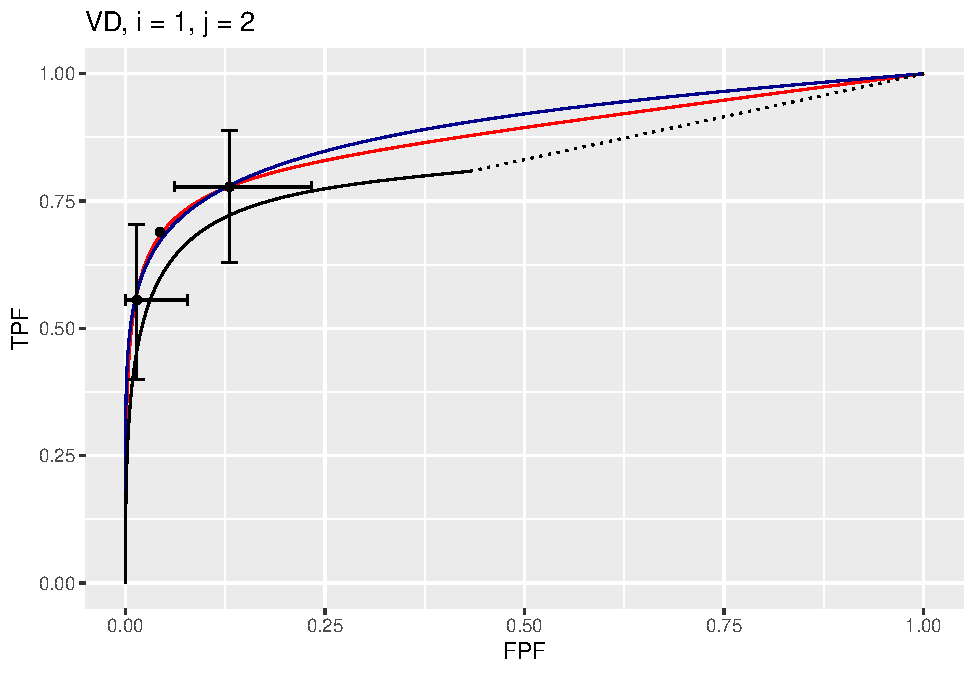
\includegraphics{11-SampleSize1_files/figure-latex/unnamed-chunk-2-1.pdf} 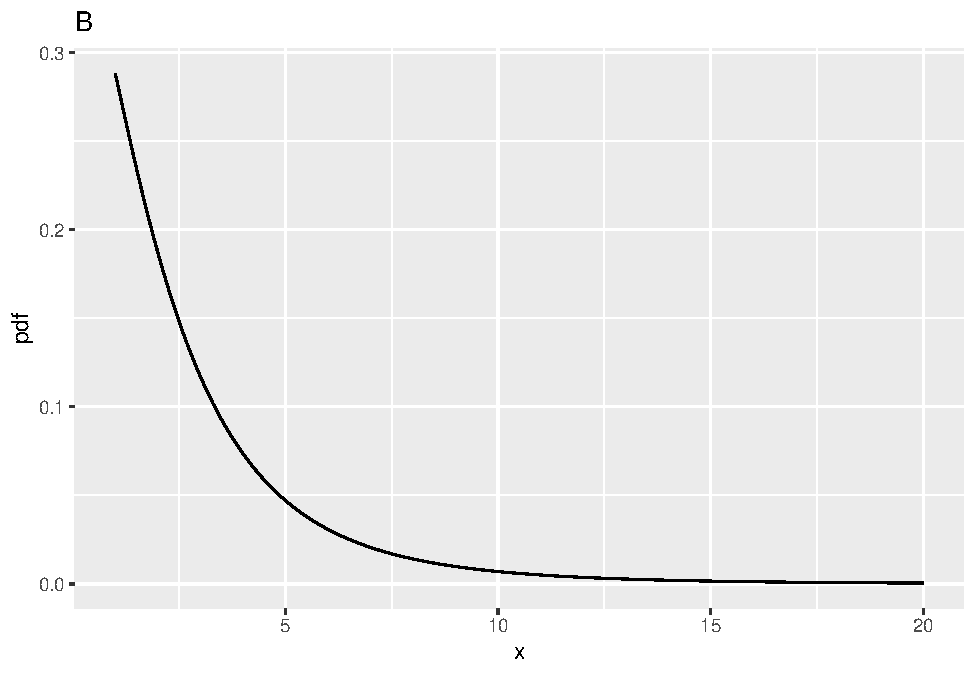
\includegraphics{11-SampleSize1_files/figure-latex/unnamed-chunk-2-2.pdf} 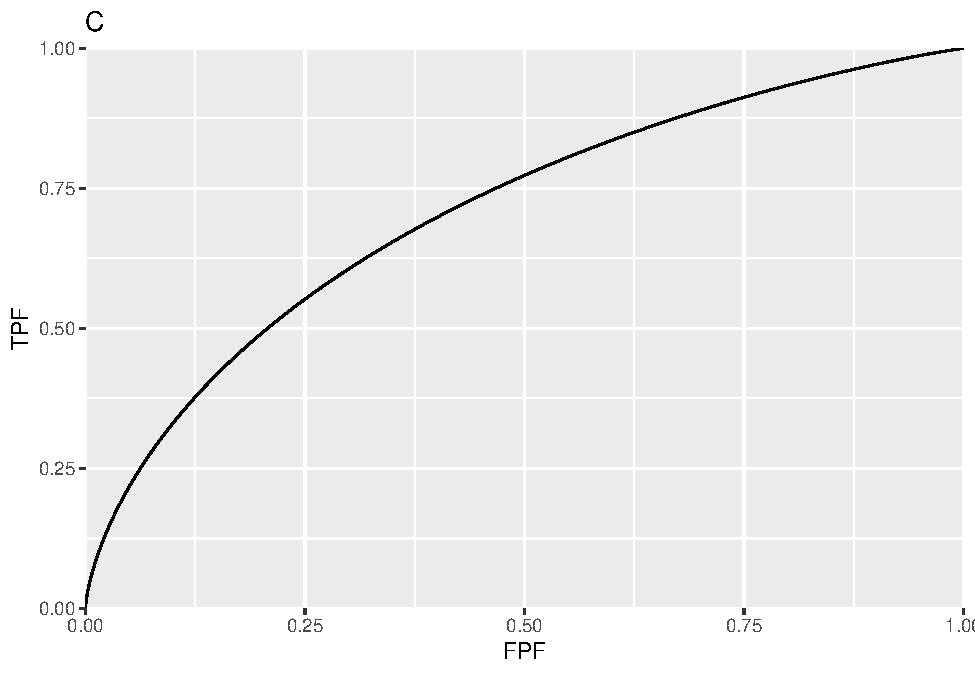
\includegraphics{11-SampleSize1_files/figure-latex/unnamed-chunk-2-3.pdf} 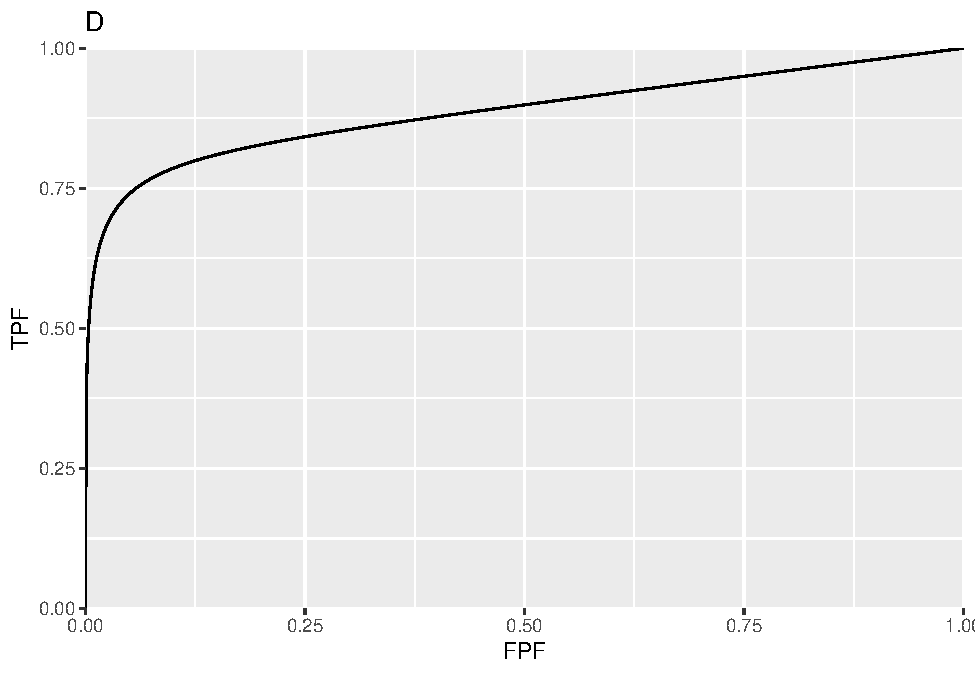
\includegraphics{11-SampleSize1_files/figure-latex/unnamed-chunk-2-4.pdf}

\begin{tabular}{l|r|r|r|r|r}
\hline
  & ndf & ddf & fCrit & ncp & pFgtFCrit\\
\hline
A & 2 & 10 & 4.102821 & 0 & 0.0500000\\
\hline
B & 2 & 10 & 4.102821 & 2 & 0.1775840\\
\hline
C & 2 & 10 & 4.102821 & 5 & 0.3876841\\
\hline
D & 2 & 10 & 4.102821 & 10 & 0.6769776\\
\hline
\end{tabular}

\hypertarget{comments}{%
\section{Comments}\label{comments}}

\hypertarget{fig.-a}{%
\subsection{Fig. A}\label{fig.-a}}

\begin{itemize}
\tightlist
\item
  This corresponds to \texttt{ncp\ =\ 0}, i.e., the \emph{central} F-distribution.
\item
  The integral under this distribution is unity (this is also true for all plots in this vignette).
\item
  The critical value, \texttt{fCrit} in the above code block, is the value of \texttt{x} such that the probability of exceeding \texttt{x} is \(\alpha\). The corresponding parameter \texttt{alpha} is defined above as 0.05.
\item
  In the current example \texttt{fCrit} = 4.102821. Notice the use of the quantile function \texttt{qf()} to determine this value, and the default value of \texttt{ncp}, namely zero, is used; specifically, one does not pass a 4th argument to \texttt{qf()}.
\item
  \textbf{The decision rule for rejecting the NH uses the NH distribution of the F-statistic}, i.e., reject the NH if F \textgreater{}= \texttt{fCrit}. As expected, \texttt{prob\ \textgreater{}\ fCrit} = 0.05 because this is how \texttt{fCrit} was defined.
\end{itemize}

\hypertarget{fig.-b}{%
\subsection{Fig. B}\label{fig.-b}}

\begin{itemize}
\tightlist
\item
  This corresponds to \texttt{ncp\ =\ 2}, \texttt{ndf} = 2 and \texttt{ddf} = 10.
\item
  The distribution is slightly shifted to the right as compared to Fig. A, thereby making it more likely that the observed value of the F-statistic will exceed the critical value determined for the NH distribution.
\item
  In fact, \texttt{prob\ \textgreater{}\ fCrit} = 0.177584, i.e., the \emph{statistical power} (compare this to Fig. A where \texttt{prob\ \textgreater{}\ fCrit} was 0.05).
\end{itemize}

\hypertarget{fig.-c}{%
\subsection{Fig. C}\label{fig.-c}}

\begin{itemize}
\tightlist
\item
  This corresponds to \texttt{ncp\ =\ 5}, \texttt{ndf} = 2 and \texttt{ddf} = 10.
\item
  Now \texttt{prob\ \textgreater{}\ fCrit} = 0.3876841.
\item
  Power has increased compared to Fig. B.
\end{itemize}

\hypertarget{fig.-d}{%
\subsection{Fig. D}\label{fig.-d}}

\begin{itemize}
\tightlist
\item
  This corresponds to \texttt{ncp\ =\ 10}, \texttt{ndf} = 2 and \texttt{ddf} = 10.
\item
  Now \texttt{prob\ \textgreater{}\ fCrit} is 0.6769776.
\item
  Power has increased compared to Fig. C.
\item
  The effect of the shift is most obvious in Fig. C and Fig. D.
\item
  Considering a vertical line at \texttt{x} = 4.102821, fraction 0.6769776 of the probability distribution in Fig. D lies to the right of this line
\item
  Therefore the NH is likely to be rejected with probability 0.6769776.
\end{itemize}

\hypertarget{summary-3}{%
\subsection{Summary}\label{summary-3}}

The larger that non-centrality parameter, the greater the shift to the right of the F-distribution, and the greater the statistical power.

\hypertarget{effect-of-ncp-for-ndf-2-and-ddf-100}{%
\section{\texorpdfstring{Effect of \texttt{ncp} for \texttt{ndf} = 2 and \texttt{ddf} = 100}{Effect of ncp for ndf = 2 and ddf = 100}}\label{effect-of-ncp-for-ndf-2-and-ddf-100}}

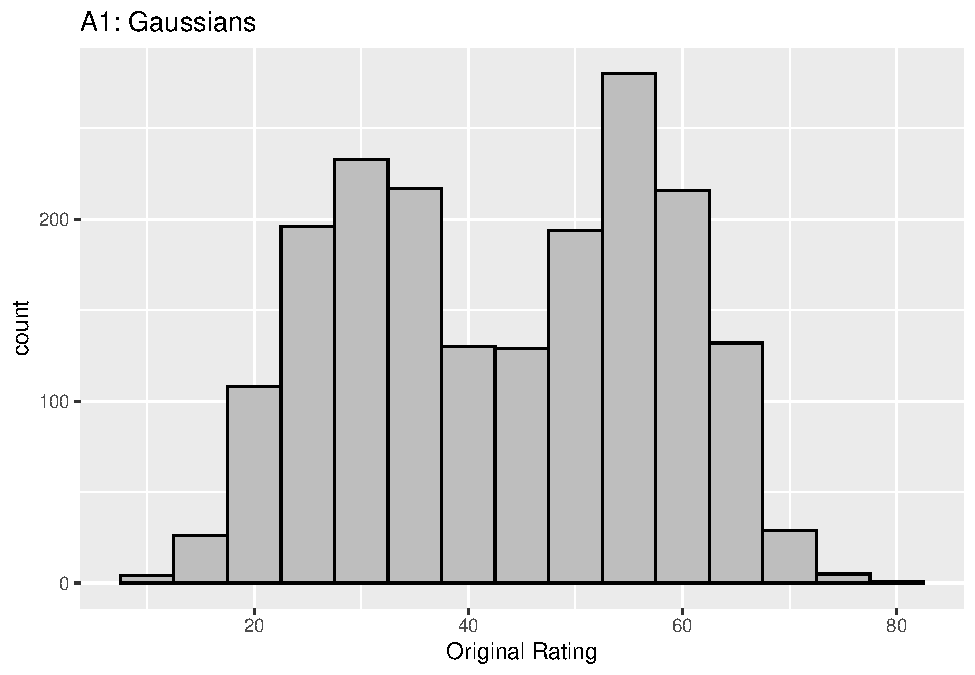
\includegraphics{11-SampleSize1_files/figure-latex/unnamed-chunk-4-1.pdf} 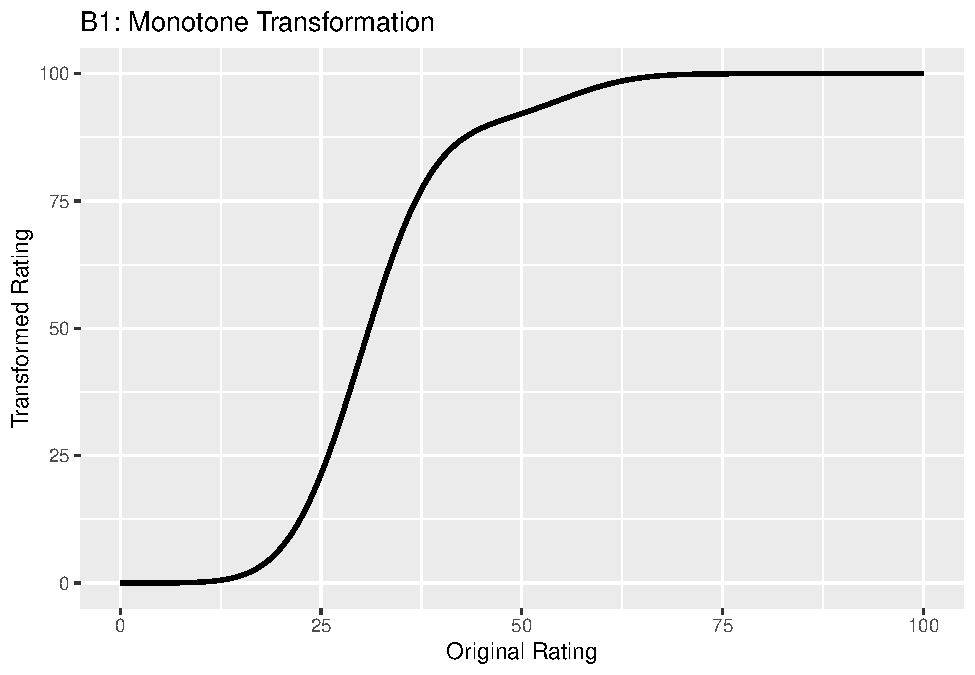
\includegraphics{11-SampleSize1_files/figure-latex/unnamed-chunk-4-2.pdf} 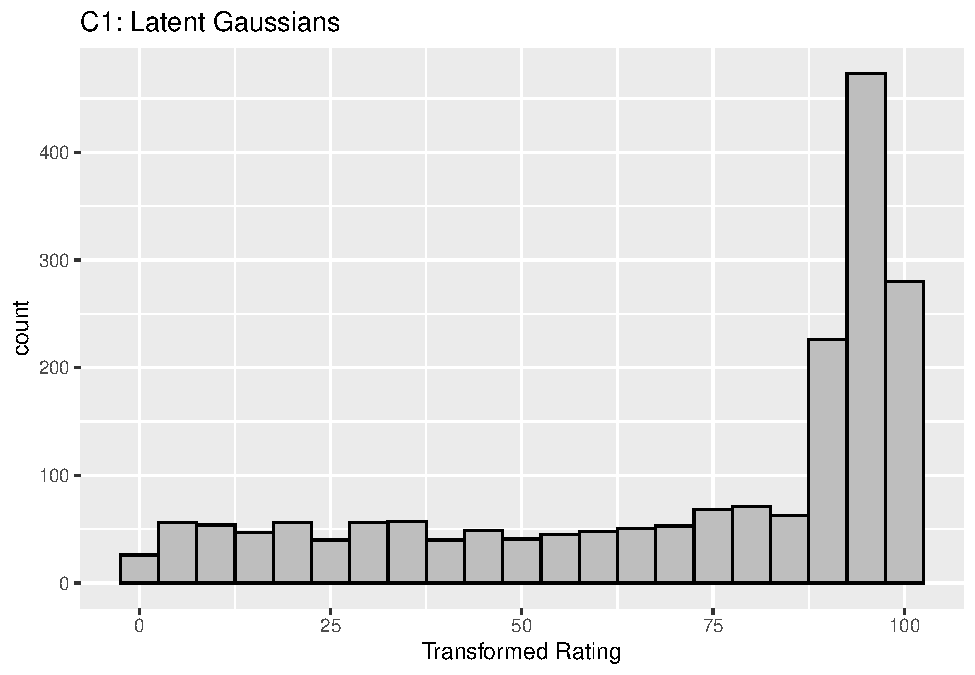
\includegraphics{11-SampleSize1_files/figure-latex/unnamed-chunk-4-3.pdf} 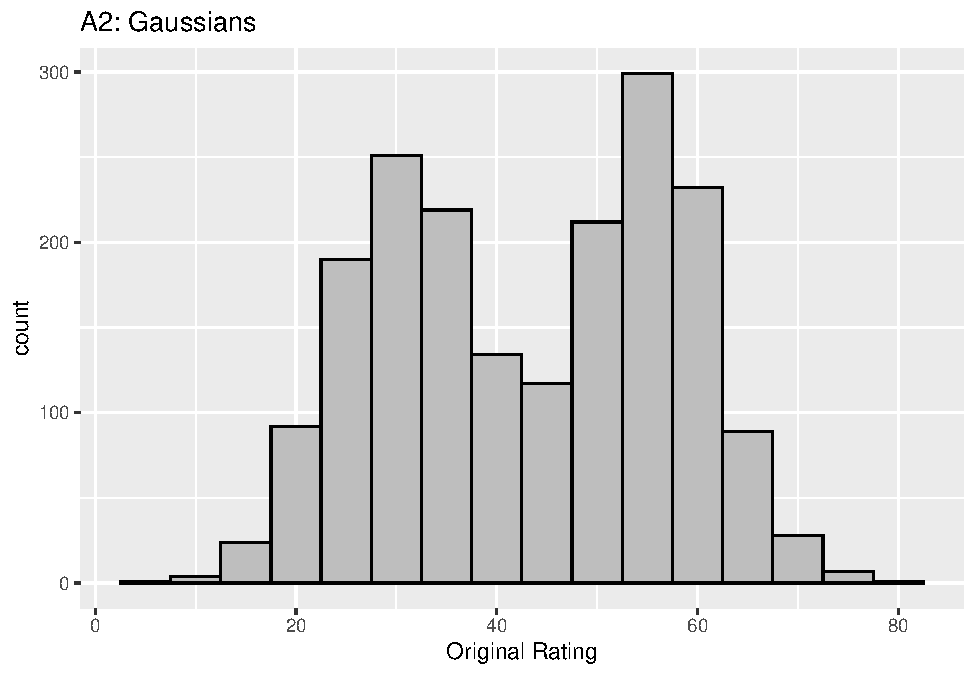
\includegraphics{11-SampleSize1_files/figure-latex/unnamed-chunk-4-4.pdf}

\begin{tabular}{l|r|r|r|r|r}
\hline
  & ndf & ddf & fCrit & ncp & pFgtFCrit\\
\hline
A & 2 & 10 & 4.102821 & 0 & 0.0500000\\
\hline
B & 2 & 10 & 4.102821 & 2 & 0.1775840\\
\hline
C & 2 & 10 & 4.102821 & 5 & 0.3876841\\
\hline
D & 2 & 10 & 4.102821 & 10 & 0.6769776\\
\hline
E & 2 & 100 & 3.087296 & 0 & 0.0500000\\
\hline
F & 2 & 100 & 3.087296 & 2 & 0.2199264\\
\hline
G & 2 & 100 & 3.087296 & 5 & 0.4910802\\
\hline
H & 2 & 100 & 3.087296 & 10 & 0.8029764\\
\hline
\end{tabular}

\hypertarget{comments-1}{%
\section{Comments}\label{comments-1}}

\begin{itemize}
\tightlist
\item
  All comparisons in this sections are at the same values of \texttt{ncp} defined above.
\item
  And between \texttt{ddf} = 100 and \texttt{ddf} = 10.
\end{itemize}

\hypertarget{fig.-e}{%
\subsection{Fig. E}\label{fig.-e}}

\begin{itemize}
\tightlist
\item
  This corresponds to \texttt{ncp} = 0, \texttt{ndf} = 2 and \texttt{ddf} = 100.
\item
  The critical value is \texttt{fCrit\_2\_100} = 3.0872959. Notice the decrease compared to the previous value for \texttt{ncp} = 0, i.e., 4.102821, for \texttt{ddf} = 10.
\item
  One expects that increasing \texttt{ddf} will make it more likely that the NH will be rejected, and this is confirmed below.
\item
  All else equal, statistical power increases with increasing \texttt{ddf}.
\end{itemize}

\hypertarget{fig.-f}{%
\subsection{Fig. F}\label{fig.-f}}

\begin{itemize}
\tightlist
\item
  This corresponds to \texttt{ncp} = 2, \texttt{ndf} = 2 and \texttt{ddf} = 100.
\item
  The probability of exceeding the critical value is \texttt{prob\ \textgreater{}\ fCrit\_2\_100} = 0.2199264, greater than the previous value, i.e., 0.177584 for \texttt{ddf} = 10.
\end{itemize}

\hypertarget{fig.-g}{%
\subsection{Fig. G}\label{fig.-g}}

\begin{itemize}
\tightlist
\item
  This corresponds to \texttt{ncp\ =\ 5}, \texttt{ndf} = 2 and \texttt{ddf} = 100.
\item
  The probability of exceeding the critical value is \texttt{prob\ \textgreater{}\ fCrit\_2\_100} = 0.4910802.
\item
  This is greater than the previous value, i.e., 0.3876841 for \texttt{ddf} = 10.
\end{itemize}

\hypertarget{fig.-h}{%
\subsection{Fig. H}\label{fig.-h}}

\begin{itemize}
\tightlist
\item
  This corresponds to \texttt{ncp\ =\ 10}, \texttt{ndf} = 2 and \texttt{ddf} = 100.
\item
  The probability of exceeding the critical value is \texttt{prob\ \textgreater{}\ fCrit\_2\_100} is 0.8029764.
\item
  This is greater than the previous value, i.e., 0.6769776 for \texttt{ddf} = 10.
\end{itemize}

\hypertarget{effect-of-ncp-for-ndf-1-ddf-100}{%
\section{\texorpdfstring{Effect of \texttt{ncp} for \texttt{ndf} = 1, \texttt{ddf} = 100}{Effect of ncp for ndf = 1, ddf = 100}}\label{effect-of-ncp-for-ndf-1-ddf-100}}

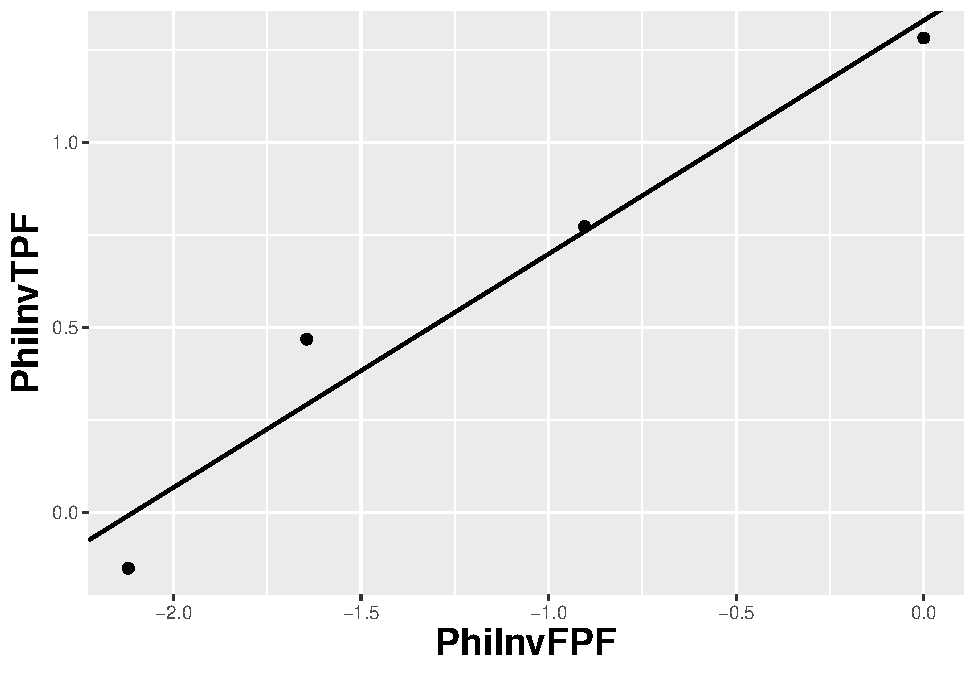
\includegraphics{11-SampleSize1_files/figure-latex/unnamed-chunk-6-1.pdf} 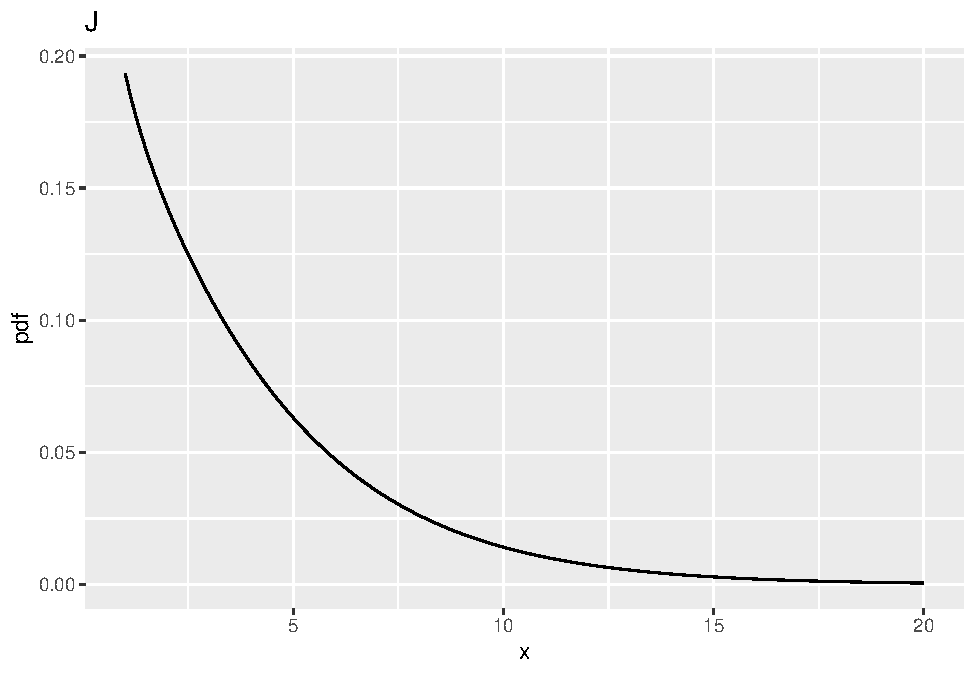
\includegraphics{11-SampleSize1_files/figure-latex/unnamed-chunk-6-2.pdf} 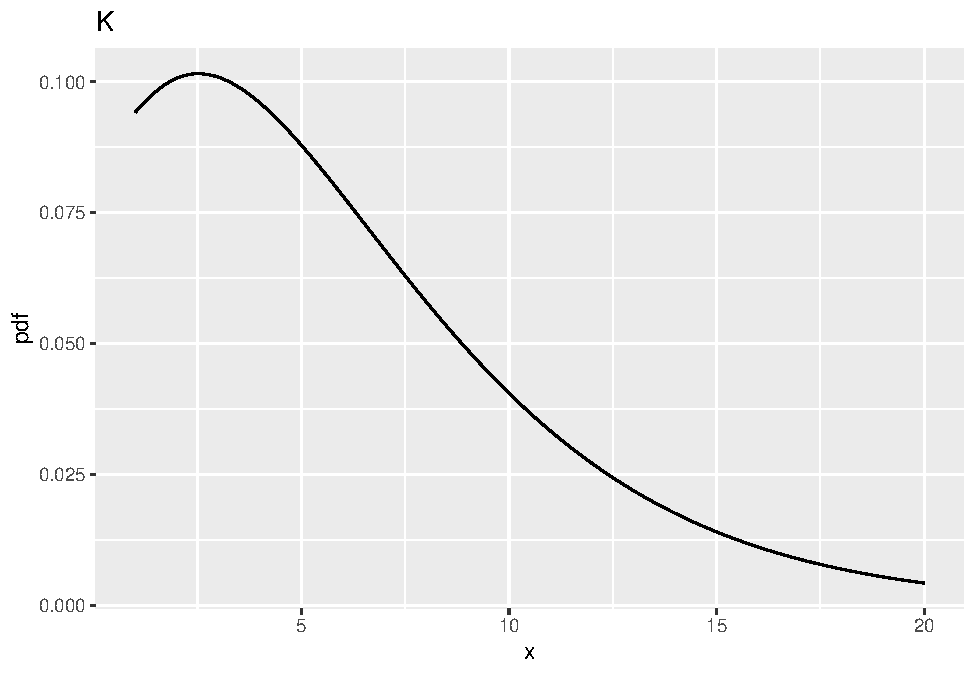
\includegraphics{11-SampleSize1_files/figure-latex/unnamed-chunk-6-3.pdf} 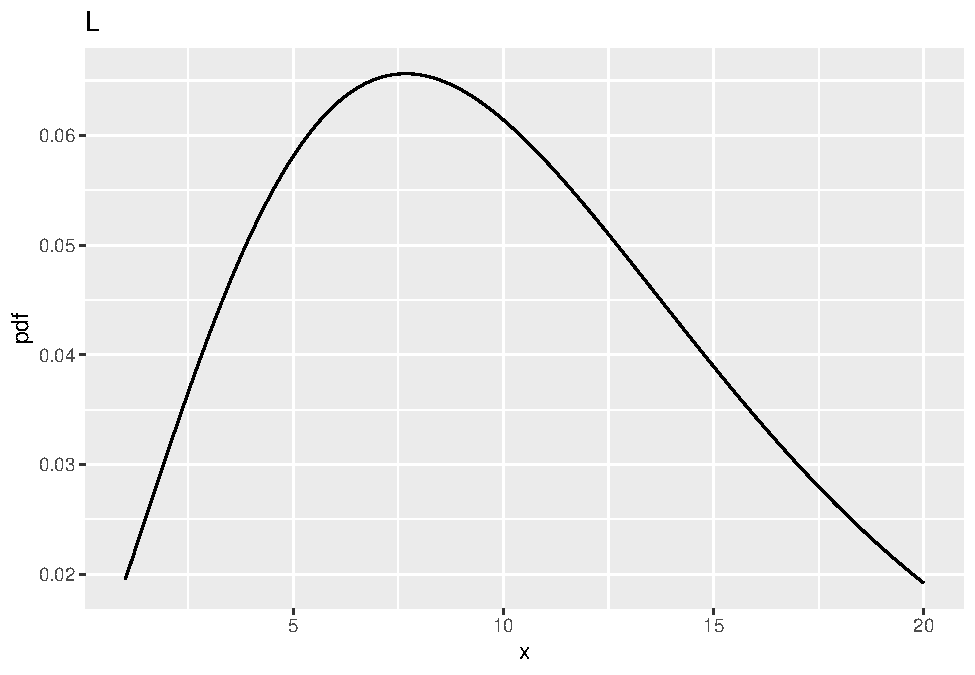
\includegraphics{11-SampleSize1_files/figure-latex/unnamed-chunk-6-4.pdf}

\begin{tabular}{l|r|r|r|r|r}
\hline
  & ndf & ddf & fCrit & ncp & pFgtFCrit\\
\hline
A & 2 & 10 & 4.102821 & 0 & 0.0500000\\
\hline
B & 2 & 10 & 4.102821 & 2 & 0.1775840\\
\hline
C & 2 & 10 & 4.102821 & 5 & 0.3876841\\
\hline
D & 2 & 10 & 4.102821 & 10 & 0.6769776\\
\hline
E & 2 & 100 & 3.087296 & 0 & 0.0500000\\
\hline
F & 2 & 100 & 3.087296 & 2 & 0.2199264\\
\hline
G & 2 & 100 & 3.087296 & 5 & 0.4910802\\
\hline
H & 2 & 100 & 3.087296 & 10 & 0.8029764\\
\hline
I & 1 & 100 & 3.936143 & 0 & 0.0500000\\
\hline
J & 1 & 100 & 3.936143 & 2 & 0.2883607\\
\hline
K & 1 & 100 & 3.936143 & 5 & 0.6004962\\
\hline
L & 1 & 100 & 3.936143 & 10 & 0.8793619\\
\hline
\end{tabular}

\hypertarget{comments-2}{%
\section{Comments}\label{comments-2}}

\begin{itemize}
\tightlist
\item
  All comparisons in this sections are at the same values of \texttt{ncp} defined above and at \texttt{ddf} = 100.
\item
  And between \texttt{ndf} = 1 and \texttt{ndf} = 2.
\end{itemize}

\hypertarget{fig.-i}{%
\subsection{Fig. I}\label{fig.-i}}

\begin{itemize}
\tightlist
\item
  This corresponds to \texttt{ncp} = 0, \texttt{ndf} = 1 and \texttt{ddf} = 100.
\item
  The critical value is \texttt{fCrit\_1\_100} = 3.936143.
\item
  Notice the increase in the critical value as compared to the corresponding value for \texttt{ndf\ =\ 2}, i.e., 3.0872959.
\item
  One might expect power to decrease, \textbf{but see below}.
\end{itemize}

\hypertarget{fig.-j}{%
\subsection{Fig. J}\label{fig.-j}}

\begin{itemize}
\tightlist
\item
  This corresponds to \texttt{ncp} = 2, \texttt{ndf} = 1 and \texttt{ddf} = 100.
\item
  Now \texttt{prob\ \textgreater{}\ fCrit\_1\_100} = 0.2883607, larger than the previous value 0.2199264.
\item
  The power has actually increased.
\end{itemize}

\hypertarget{fig.-k}{%
\subsection{Fig. K}\label{fig.-k}}

\begin{itemize}
\tightlist
\item
  This corresponds to \texttt{ncp} = 5, \texttt{ndf} = 1 and \texttt{ddf} = 100`',
\item
  Now \texttt{prob\ \textgreater{}\ fCrit\_1\_100} = 0.6004962, larger than the previous value 0.4910802.
\item
  Again, the power has actually increased.
\end{itemize}

\hypertarget{fig.-l}{%
\subsection{Fig. L}\label{fig.-l}}

\begin{itemize}
\tightlist
\item
  This corresponds to \texttt{ncp} = 10, \texttt{ndf} = 1 and \texttt{ddf} = 100
\item
  Now \texttt{prob\ \textgreater{}\ fCrit\_1\_100} is 0.8793619, larger than the previous value 0.8029764.
\item
  The power has actually increased.
\end{itemize}

\hypertarget{summary-4}{%
\section{Summary}\label{summary-4}}

\begin{itemize}
\tightlist
\item
  Power increases with increasing \texttt{ddf} and \texttt{ncp}.
\item
  The effect of increasing \texttt{ncp} is quite dramatic. This is because power depends on the square of \texttt{ncp}.
\item
  Decreasing \texttt{ndf} also \textbf{increases} power. At first glance this may seem counterintuitive, as \texttt{fCrit} has gone up, but is explained by the differing shapes of the two distributions: the pdf is broader for \texttt{ndf} = 1 as compared to \texttt{ndf} = 2 (compare Fig. L to H).
\end{itemize}

\hypertarget{references-6}{%
\section{References}\label{references-6}}

\hypertarget{SSRocFirstPrinciples}{%
\chapter{ROC-DBMH sample size from first principles}\label{SSRocFirstPrinciples}}

\hypertarget{introduction-7}{%
\section{Introduction}\label{introduction-7}}

The starting point is a \textbf{pilot} study. The variability in this dataset (specifically the variance components, subsequently converted to mean squares), obtained by running the significance testing function \texttt{StSignificanceTesting()}, is used to extrapolate to the necessary numbers of readers and cases, in the \textbf{pivotal} study, to achieve the desired power. In this example, the observed effect size in the pilot study is used as the anticipated effect size for the pivotal study -- this is generally not a good idea as discussed in \textbf{Chapter 11} under ``Cautionary notes''. Shown below, and the reader should confirm, is a first principles implementation of the relevant formulae in \textbf{Chapter 11}.

\hypertarget{sample-size-estimation-using-the-dbmh-method}{%
\section{Sample size estimation using the DBMH method}\label{sample-size-estimation-using-the-dbmh-method}}

The Van Dyke dataset in file \texttt{VanDyke.lrc}, in \texttt{"MRMC"} format, is regarded as a pilot study. The command \texttt{rocData\ \textless{}-\ DfReadDataFile(fileName,\ format\ =\ "MRMC")} reads the data and saves it to a \texttt{dataset} object \texttt{rocData}. \href{https://dpc10ster.github.io/RJafroc/reference/RJafroc-package.html}{For more on data formats click here}. The next line uses the function \texttt{StSignificanceTesting()} to apply \texttt{method\ =\ "DBMH"} analysis, the default, using the \texttt{FOM\ =\ "Wilcoxon"} figure of merit. The next line extracts the variance components \texttt{varYTR}, \texttt{varYTC} and \texttt{varYEps} (the Y's denote pseudovalue based values). The next line extracts the effect size.

\begin{Shaded}
\begin{Highlighting}[]
\NormalTok{alpha <-}\StringTok{ }\FloatTok{0.05}
\NormalTok{rocData <-}\StringTok{ }\NormalTok{dataset02 }\CommentTok{##"VanDyke.lrc"}
\CommentTok{#fileName <- dataset03 ## "Franken1.lrc"}
\NormalTok{retDbm <-}\StringTok{ }\KeywordTok{StSignificanceTesting}\NormalTok{(}\DataTypeTok{dataset =}\NormalTok{ rocData, }\DataTypeTok{FOM =} \StringTok{"Wilcoxon"}\NormalTok{, }\DataTypeTok{method =} \StringTok{"DBMH"}\NormalTok{) }
\NormalTok{varYTR <-}\StringTok{ }\NormalTok{retDbm}\OperatorTok{$}\NormalTok{varComp}\OperatorTok{$}\NormalTok{varTR;varYTC <-}\StringTok{ }\NormalTok{retDbm}\OperatorTok{$}\NormalTok{varComp}\OperatorTok{$}\NormalTok{varTC;varYEps <-}\StringTok{ }\NormalTok{retDbm}\OperatorTok{$}\NormalTok{varComp}\OperatorTok{$}\NormalTok{varErr}
\NormalTok{effectSize <-}\StringTok{ }\NormalTok{retDbm}\OperatorTok{$}\NormalTok{ciDiffTrtRRRC}\OperatorTok{$}\NormalTok{Estimate}
\end{Highlighting}
\end{Shaded}

The \emph{observed} effect size is \texttt{effectSize} = -0.0438003, which, in this example, is used as the \emph{anticipated} effect size, generally not a good idea. \textbf{See Chapter 11 for nuances regarding the choice of this all important value.} The following code snippet reveals the names and array indexing of the pseudovalue variance components.

\begin{Shaded}
\begin{Highlighting}[]
\NormalTok{retDbm}\OperatorTok{$}\NormalTok{varComp}
\CommentTok{#>          varR       varC        varTR     varTC      varRC    varErr}
\CommentTok{#> 1 0.001534999 0.02724923 0.0002004025 0.0119753 0.01226473 0.0399716}
\end{Highlighting}
\end{Shaded}

For example, the treatment-reader pseudovalue variance component is the third element of \texttt{retDbm\$varComp}.

\hypertarget{random-reader-random-case-rrrc}{%
\subsection{Random reader random case (RRRC)}\label{random-reader-random-case-rrrc}}

This illustrates random reader random case sample size estimation. Assumed are 10 readers and 163 cases in the pivotal study. The non-centrality parameter is defined by:

\[\Delta =\frac{JK\sigma _{Y;\tau }^{2}}{\left( \sigma _{Y;\varepsilon }^{2}+\sigma _{Y;\tau RC}^{2} \right)+K\sigma _{Y;\tau R}^{2}+J\max \left( \sigma _{Y;\tau C}^{2},0 \right)}\]

The sampling distribution of the F-statistic under the AH is:

\[{{F}_{\left. AH \right|R}}\equiv \frac{MST}{MSTC}\tilde{\ }{{F}_{I-1,\left( I-1 \right)\left( K-1 \right),\Delta }}\]
Also,

\[\sigma _{Y;\tau }^{2}={{d}^{2}}/2\]

where \texttt{d} is the observed effect size, i.e., \texttt{effectSize}. The formulae for calculating the mean-squares are in \citep{RN1476}, implemented in \texttt{UtilMeanSquares()}.

\begin{Shaded}
\begin{Highlighting}[]
\CommentTok{#RRRC}
\NormalTok{J <-}\StringTok{ }\DecValTok{10}\NormalTok{;K <-}\StringTok{ }\DecValTok{163}
\NormalTok{ncp <-}\StringTok{ }\NormalTok{(}\FloatTok{0.5}\OperatorTok{*}\NormalTok{J}\OperatorTok{*}\NormalTok{K}\OperatorTok{*}\NormalTok{(effectSize)}\OperatorTok{^}\DecValTok{2}\NormalTok{)}\OperatorTok{/}\NormalTok{(K}\OperatorTok{*}\NormalTok{varYTR}\OperatorTok{+}\KeywordTok{max}\NormalTok{(J}\OperatorTok{*}\NormalTok{varYTC,}\DecValTok{0}\NormalTok{)}\OperatorTok{+}\NormalTok{varYEps)}
\NormalTok{MS <-}\StringTok{ }\KeywordTok{UtilMeanSquares}\NormalTok{(rocData, }\DataTypeTok{FOM =} \StringTok{"Wilcoxon"}\NormalTok{, }\DataTypeTok{method =} \StringTok{"DBMH"}\NormalTok{)}
\NormalTok{ddf <-}\StringTok{ }\NormalTok{(MS}\OperatorTok{$}\NormalTok{msTR}\OperatorTok{+}\KeywordTok{max}\NormalTok{(MS}\OperatorTok{$}\NormalTok{msTC}\OperatorTok{-}\NormalTok{MS}\OperatorTok{$}\NormalTok{msTRC,}\DecValTok{0}\NormalTok{))}\OperatorTok{^}\DecValTok{2}\OperatorTok{/}\NormalTok{(MS}\OperatorTok{$}\NormalTok{msTR}\OperatorTok{^}\DecValTok{2}\NormalTok{)}\OperatorTok{*}\NormalTok{(J}\DecValTok{-1}\NormalTok{)}
\NormalTok{FCrit <-}\StringTok{ }\KeywordTok{qf}\NormalTok{(}\DecValTok{1} \OperatorTok{-}\StringTok{ }\NormalTok{alpha, }\DecValTok{1}\NormalTok{, ddf)}
\NormalTok{Power1 <-}\StringTok{ }\DecValTok{1}\OperatorTok{-}\KeywordTok{pf}\NormalTok{(FCrit, }\DecValTok{1}\NormalTok{, ddf, }\DataTypeTok{ncp =}\NormalTok{ ncp)}
\end{Highlighting}
\end{Shaded}

The next line calculates the non centrality parameter, \texttt{ncp} = 8.1269825. Note that \texttt{effectSize} enters as the \textbf{square}. The \texttt{UtilMeanSquares()} function returns the mean-squares as a \texttt{list} (ignore the last two rows of output for now).

\begin{Shaded}
\begin{Highlighting}[]
\KeywordTok{str}\NormalTok{(MS)}
\CommentTok{#> List of 9}
\CommentTok{#>  $ msT       : num 0.547}
\CommentTok{#>  $ msR       : num 0.437}
\CommentTok{#>  $ msC       : num 0.397}
\CommentTok{#>  $ msTR      : num 0.0628}
\CommentTok{#>  $ msTC      : num 0.0521}
\CommentTok{#>  $ msRC      : num 0.0645}
\CommentTok{#>  $ msTRC     : num 0.04}
\CommentTok{#>  $ msCSingleT: num [1:2] 0.336 0.16}
\CommentTok{#>  $ msCSingleR: num [1:5] 0.1222 0.2127 0.1365 0.0173 0.1661}
\end{Highlighting}
\end{Shaded}

The next line calculates \texttt{ddf} = 12.822129. The remaining lines calculate the critical value of the F-distribution, \texttt{FCrit} = 4.680382 and statistical power = 0.7494133, which by design is close to 80\%, i.e., the numbers of readers and cases were chosen to achieve this value.

\hypertarget{fixed-reader-random-case-frrc}{%
\subsection{Fixed reader random case (FRRC)}\label{fixed-reader-random-case-frrc}}

This code illustrates fixed reader random case sample size estimation. Assumed are 10 readers and 133 cases in the pivotal study. The formulae are:

\[\Delta =\frac{JK\sigma _{Y;\tau }^{2}}{\sigma _{Y;\varepsilon }^{2}+\sigma _{Y;\tau RC}^{2}+J\sigma _{Y;\tau C}^{2}}\]

The sampling distribution of the F-statistic under the AH is:

\[{{F}_{\left. AH \right|R}}\equiv \frac{MST}{MSTC}\tilde{\ }{{F}_{I-1,\left( I-1 \right)\left( K-1 \right),\Delta }}\]

\begin{Shaded}
\begin{Highlighting}[]
\CommentTok{#FRRC}
\NormalTok{ncp <-}\StringTok{ }\NormalTok{(}\FloatTok{0.5}\OperatorTok{*}\NormalTok{J}\OperatorTok{*}\NormalTok{K}\OperatorTok{*}\NormalTok{(effectSize)}\OperatorTok{^}\DecValTok{2}\NormalTok{)}\OperatorTok{/}\NormalTok{(}\KeywordTok{max}\NormalTok{(J}\OperatorTok{*}\NormalTok{varYTC,}\DecValTok{0}\NormalTok{)}\OperatorTok{+}\NormalTok{varYEps)}
\NormalTok{ddf <-}\StringTok{ }\NormalTok{(K}\DecValTok{-1}\NormalTok{)}
\NormalTok{FCrit <-}\StringTok{ }\KeywordTok{qf}\NormalTok{(}\DecValTok{1} \OperatorTok{-}\StringTok{ }\NormalTok{alpha, }\DecValTok{1}\NormalTok{, ddf)}
\NormalTok{Power2 <-}\StringTok{ }\DecValTok{1}\OperatorTok{-}\KeywordTok{pf}\NormalTok{(FCrit, }\DecValTok{1}\NormalTok{, ddf, }\DataTypeTok{ncp =}\NormalTok{ ncp)}
\end{Highlighting}
\end{Shaded}

This time non centrality parameter, \texttt{ncp} = 7.9873835, \texttt{ddf} = 132, \texttt{FCrit} = 3.912875 and statistical power = 0.8011167. Again, be design, this is close to 80\%. Note that when readers are regarded as a fixed effect, fewer cases are needed to achieve the desired power. Freezing out a source of variability results in a more stable measurement and hence fewer cases are needed to achieve the desired power.

\hypertarget{random-reader-fixed-case-rrfc}{%
\subsection{Random reader fixed case (RRFC)}\label{random-reader-fixed-case-rrfc}}

This code illustrates random reader random case sample size estimation. Assumed are 10 readers and 53 cases in the pivotal study. The formulae are:

\[\Delta =\frac{JK\sigma _{Y;\tau }^{2}}{\sigma _{Y;\varepsilon }^{2}+\sigma _{Y;\tau RC}^{2}+K\sigma _{Y;\tau R}^{2}}\]

The sampling distribution of the F-statistic under the AH is:

\[{{F}_{\left. AH \right|C}}\equiv \frac{MST}{MSTR}\tilde{\ }{{F}_{I-1,\left( I-1 \right)\left( J-1 \right),\Delta }}\]

\begin{Shaded}
\begin{Highlighting}[]
\CommentTok{#RRFC}
\NormalTok{ncp <-}\StringTok{ }\NormalTok{(}\FloatTok{0.5}\OperatorTok{*}\NormalTok{J}\OperatorTok{*}\NormalTok{K}\OperatorTok{*}\NormalTok{(effectSize)}\OperatorTok{^}\DecValTok{2}\NormalTok{)}\OperatorTok{/}\NormalTok{(K}\OperatorTok{*}\NormalTok{varYTR}\OperatorTok{+}\NormalTok{varYEps)}
\NormalTok{ddf <-}\StringTok{ }\NormalTok{(J}\DecValTok{-1}\NormalTok{)}
\NormalTok{FCrit <-}\StringTok{ }\KeywordTok{qf}\NormalTok{(}\DecValTok{1} \OperatorTok{-}\StringTok{ }\NormalTok{alpha, }\DecValTok{1}\NormalTok{, ddf)}
\NormalTok{Power3 <-}\StringTok{ }\DecValTok{1}\OperatorTok{-}\KeywordTok{pf}\NormalTok{(FCrit, }\DecValTok{1}\NormalTok{, ddf, }\DataTypeTok{ncp =}\NormalTok{ ncp)}
\end{Highlighting}
\end{Shaded}

This time non centrality parameter, \texttt{ncp} = 10.0487164, \texttt{ddf} = 9, \texttt{FCrit} = 5.117355 and statistical power = 0.8049666. Again, be design, this is close to 80\%.

\hypertarget{summary-5}{%
\section{Summary}\label{summary-5}}

For 10 readers, the numbers of cases needed for 80\% power is largest (163) for RRRC, intermediate (133) for FRRC and least for RRFC (53). For all three analyses, the expectation of 80\% power is met.

\hypertarget{references-7}{%
\section{References}\label{references-7}}

\hypertarget{SSRocDBMHRJafroc}{%
\chapter{ROC-DBMH sample size using RJafroc}\label{SSRocDBMHRJafroc}}

\hypertarget{introduction-8}{%
\section{Introduction}\label{introduction-8}}

This illustrates the \texttt{RJafroc} implementation of sample-size estimation. Default \(\alpha\) is 0.05 and default power (1-\(\beta\)) is 0.8. Three functions are provided. Each of these functions can be used with \texttt{method\ "DBMH"} (illustrated here, the default) or \texttt{method\ =\ "ORH"} (next vignette). Illustrated below, for the most part, is the random-reader random-case (RRRC) option, i.e., \texttt{option\ =\ "RRRC"}. The last two examples illustrate fixed-reader random-case (FRRC) \texttt{option\ =\ "FRRC"} and random-reader fixed-case (RRFC) \texttt{option\ =\ "RRFC"} options.

\begin{itemize}
\tightlist
\item
  \texttt{SsPowerGivenJK()}
  Statistical power for specified numbers of readers and cases in an ROC study.
\item
  \texttt{SsPowerTable()}
  Generate a power table, i.e., combinations of numbers of readers and cases yielding the desired power.
\item
  \texttt{SsSampleSizeKGivenJ}
  Number of cases, for specified number of readers, to achieve desired power.
\end{itemize}

\hypertarget{illustration-of-sspowergivenjk-using-method-dbmh}{%
\section{\texorpdfstring{Illustration of \texttt{SsPowerGivenJK()} using \texttt{method\ =\ "DBMH"}}{Illustration of SsPowerGivenJK() using method = "DBMH"}}\label{illustration-of-sspowergivenjk-using-method-dbmh}}

The selected dataset corresponds to the Van Dyke data.

\begin{Shaded}
\begin{Highlighting}[]
\NormalTok{power <-}\StringTok{ }\KeywordTok{SsPowerGivenJK}\NormalTok{(dataset02, }\DataTypeTok{FOM =} \StringTok{"Wilcoxon"}\NormalTok{, }\DataTypeTok{J =} \DecValTok{6}\NormalTok{, }\DataTypeTok{K =} \DecValTok{112}\NormalTok{, }\DataTypeTok{option =} \StringTok{"RRRC"}\NormalTok{)}
\end{Highlighting}
\end{Shaded}

The returned value is a list containing the expected power \texttt{power}, the non-centrality parameter \texttt{ncp}, the denominator degrees of freedom \texttt{ddf} and the F-statistic \texttt{f}. The numerator degrees of freedom \texttt{ndf} is always \texttt{I\ -\ 1}, i.e., unity for this dataset.

\begin{Shaded}
\begin{Highlighting}[]
\KeywordTok{str}\NormalTok{(power)}
\CommentTok{#> 'data.frame':    1 obs. of  4 variables:}
\CommentTok{#>  $ powerRRRC: num 0.556}
\CommentTok{#>  $ ncpRRRC  : num 4.8}
\CommentTok{#>  $ ddfHRRRC : num 23.1}
\CommentTok{#>  $ fRRRC    : num 4.28}
\end{Highlighting}
\end{Shaded}

Expected power is 0.5555789.

\hypertarget{illustration-of-sspowertable-using-method-dbmh}{%
\section{\texorpdfstring{Illustration of \texttt{SsPowerTable()} using \texttt{method\ =\ "DBMH"}}{Illustration of SsPowerTable() using method = "DBMH"}}\label{illustration-of-sspowertable-using-method-dbmh}}

\begin{Shaded}
\begin{Highlighting}[]
\NormalTok{powTab <-}\StringTok{ }\KeywordTok{SsPowerTable}\NormalTok{(dataset02, }\DataTypeTok{FOM =} \StringTok{"Wilcoxon"}\NormalTok{, }\DataTypeTok{method =} \StringTok{"DBMH"}\NormalTok{, }\DataTypeTok{option =} \StringTok{"RRRC"}\NormalTok{)}
\end{Highlighting}
\end{Shaded}

Now show the power table \texttt{powTab}. Note that the last column is always close to 0.8, the desired power. The 2nd and 3rd columns show the number of readers and number of cases to achieve the desired power.

\begin{Shaded}
\begin{Highlighting}[]
\NormalTok{powTab}
\CommentTok{#>     numReaders numCases power}
\CommentTok{#> 1            3    >2000  <NA>}
\CommentTok{#> 2            3    >2000  <NA>}
\CommentTok{#> 3            4     1089   0.8}
\CommentTok{#> 4            4     1089   0.8}
\CommentTok{#> 5            5      344 0.801}
\CommentTok{#> 6            5      344 0.801}
\CommentTok{#> 7            6      251 0.801}
\CommentTok{#> 8            6      251 0.801}
\CommentTok{#> 9            7      211 0.801}
\CommentTok{#> 10           7      211 0.801}
\CommentTok{#> 11           8      188 0.801}
\CommentTok{#> 12           8      188 0.801}
\CommentTok{#> 13           9      173 0.801}
\CommentTok{#> 14           9      173 0.801}
\CommentTok{#> 15          10      163 0.802}
\CommentTok{#> 16          10      163 0.802}
\CommentTok{#> 17          11      155 0.801}
\CommentTok{#> 18          11      155 0.801}
\CommentTok{#> 19          12      149 0.802}
\CommentTok{#> 20          12      149 0.802}
\CommentTok{#> 21          13      144 0.801}
\CommentTok{#> 22          13      144 0.801}
\CommentTok{#> 23          14      140 0.802}
\CommentTok{#> 24          14      140 0.802}
\CommentTok{#> 25          15      137 0.802}
\CommentTok{#> 26          15      137 0.802}
\CommentTok{#> 27          16      134 0.802}
\CommentTok{#> 28          16      134 0.802}
\CommentTok{#> 29          17      131 0.801}
\CommentTok{#> 30          17      131 0.801}
\CommentTok{#> 31          18      129 0.801}
\CommentTok{#> 32          18      129 0.801}
\CommentTok{#> 33          19      127 0.801}
\CommentTok{#> 34          19      127 0.801}
\CommentTok{#> 35          20      126 0.802}
\CommentTok{#> 36          20      126 0.802}
\CommentTok{#> 37          21      124 0.801}
\CommentTok{#> 38          21      124 0.801}
\CommentTok{#> 39          22      123 0.802}
\CommentTok{#> 40          22      123 0.802}
\CommentTok{#> 41          23      122 0.802}
\CommentTok{#> 42          23      122 0.802}
\CommentTok{#> 43          24      121 0.803}
\CommentTok{#> 44          24      121 0.803}
\CommentTok{#> 45          25      120 0.802}
\CommentTok{#> 46          25      120 0.802}
\CommentTok{#> 47          26      119 0.802}
\CommentTok{#> 48          26      119 0.802}
\CommentTok{#> 49          27      118 0.802}
\CommentTok{#> 50          27      118 0.802}
\CommentTok{#> 51          28      117 0.801}
\CommentTok{#> 52          28      117 0.801}
\CommentTok{#> 53          29      117 0.803}
\CommentTok{#> 54          29      117 0.803}
\CommentTok{#> 55          30      116 0.802}
\CommentTok{#> 56          30      116 0.802}
\CommentTok{#> 57          31      115 0.801}
\CommentTok{#> 58          31      115 0.801}
\CommentTok{#> 59          32      115 0.803}
\CommentTok{#> 60          32      115 0.803}
\CommentTok{#> 61          33      114 0.801}
\CommentTok{#> 62          33      114 0.801}
\CommentTok{#> 63          34      114 0.803}
\CommentTok{#> 64          34      114 0.803}
\CommentTok{#> 65          35      113 0.801}
\CommentTok{#> 66          35      113 0.801}
\CommentTok{#> 67          36      113 0.802}
\CommentTok{#> 68          36      113 0.802}
\CommentTok{#> 69          37      112   0.8}
\CommentTok{#> 70          37      112   0.8}
\CommentTok{#> 71          38      112 0.802}
\CommentTok{#> 72          38      112 0.802}
\CommentTok{#> 73          39      112 0.803}
\CommentTok{#> 74          39      112 0.803}
\CommentTok{#> 75          40      111 0.801}
\CommentTok{#> 76          40      111 0.801}
\CommentTok{#> 77          41      111 0.802}
\CommentTok{#> 78          41      111 0.802}
\CommentTok{#> 79          42      111 0.803}
\CommentTok{#> 80          42      111 0.803}
\CommentTok{#> 81          43      110 0.801}
\CommentTok{#> 82          43      110 0.801}
\CommentTok{#> 83          44      110 0.802}
\CommentTok{#> 84          44      110 0.802}
\CommentTok{#> 85          45      110 0.802}
\CommentTok{#> 86          45      110 0.802}
\CommentTok{#> 87          46      110 0.803}
\CommentTok{#> 88          46      110 0.803}
\CommentTok{#> 89          47      109 0.801}
\CommentTok{#> 90          47      109 0.801}
\CommentTok{#> 91          48      109 0.802}
\CommentTok{#> 92          48      109 0.802}
\CommentTok{#> 93          49      109 0.802}
\CommentTok{#> 94          49      109 0.802}
\CommentTok{#> 95          50      109 0.803}
\CommentTok{#> 96          50      109 0.803}
\CommentTok{#> 97          51      108   0.8}
\CommentTok{#> 98          51      108   0.8}
\CommentTok{#> 99          52      108 0.801}
\CommentTok{#> 100         52      108 0.801}
\CommentTok{#> 101         53      108 0.802}
\CommentTok{#> 102         53      108 0.802}
\CommentTok{#> 103         54      108 0.802}
\CommentTok{#> 104         54      108 0.802}
\CommentTok{#> 105         55      108 0.803}
\CommentTok{#> 106         55      108 0.803}
\CommentTok{#> 107         56      107   0.8}
\CommentTok{#> 108         56      107   0.8}
\CommentTok{#> 109         57      107 0.801}
\CommentTok{#> 110         57      107 0.801}
\CommentTok{#> 111         58      107 0.801}
\CommentTok{#> 112         58      107 0.801}
\CommentTok{#> 113         59      107 0.802}
\CommentTok{#> 114         59      107 0.802}
\CommentTok{#> 115         60      107 0.802}
\CommentTok{#> 116         60      107 0.802}
\CommentTok{#> 117         61      107 0.803}
\CommentTok{#> 118         61      107 0.803}
\CommentTok{#> 119         62      107 0.803}
\CommentTok{#> 120         62      107 0.803}
\CommentTok{#> 121         63      106   0.8}
\CommentTok{#> 122         63      106   0.8}
\CommentTok{#> 123         64      106 0.801}
\CommentTok{#> 124         64      106 0.801}
\CommentTok{#> 125         65      106 0.801}
\CommentTok{#> 126         65      106 0.801}
\CommentTok{#> 127         66      106 0.802}
\CommentTok{#> 128         66      106 0.802}
\CommentTok{#> 129         67      106 0.802}
\CommentTok{#> 130         67      106 0.802}
\CommentTok{#> 131         68      106 0.802}
\CommentTok{#> 132         68      106 0.802}
\CommentTok{#> 133         69      106 0.803}
\CommentTok{#> 134         69      106 0.803}
\CommentTok{#> 135         70      106 0.803}
\CommentTok{#> 136         70      106 0.803}
\CommentTok{#> 137         71      106 0.804}
\CommentTok{#> 138         71      106 0.804}
\CommentTok{#> 139         72      105   0.8}
\CommentTok{#> 140         72      105   0.8}
\CommentTok{#> 141         73      105 0.801}
\CommentTok{#> 142         73      105 0.801}
\CommentTok{#> 143         74      105 0.801}
\CommentTok{#> 144         74      105 0.801}
\CommentTok{#> 145         75      105 0.801}
\CommentTok{#> 146         75      105 0.801}
\CommentTok{#> 147         76      105 0.802}
\CommentTok{#> 148         76      105 0.802}
\CommentTok{#> 149         77      105 0.802}
\CommentTok{#> 150         77      105 0.802}
\CommentTok{#> 151         78      105 0.802}
\CommentTok{#> 152         78      105 0.802}
\CommentTok{#> 153         79      105 0.803}
\CommentTok{#> 154         79      105 0.803}
\CommentTok{#> 155         80      105 0.803}
\CommentTok{#> 156         80      105 0.803}
\CommentTok{#> 157         81      105 0.803}
\CommentTok{#> 158         81      105 0.803}
\CommentTok{#> 159         82      105 0.803}
\CommentTok{#> 160         82      105 0.803}
\CommentTok{#> 161         83      104   0.8}
\CommentTok{#> 162         83      104   0.8}
\CommentTok{#> 163         84      104   0.8}
\CommentTok{#> 164         84      104   0.8}
\CommentTok{#> 165         85      104 0.801}
\CommentTok{#> 166         85      104 0.801}
\CommentTok{#> 167         86      104 0.801}
\CommentTok{#> 168         86      104 0.801}
\CommentTok{#> 169         87      104 0.801}
\CommentTok{#> 170         87      104 0.801}
\CommentTok{#> 171         88      104 0.801}
\CommentTok{#> 172         88      104 0.801}
\CommentTok{#> 173         89      104 0.802}
\CommentTok{#> 174         89      104 0.802}
\CommentTok{#> 175         90      104 0.802}
\CommentTok{#> 176         90      104 0.802}
\CommentTok{#> 177         91      104 0.802}
\CommentTok{#> 178         91      104 0.802}
\CommentTok{#> 179         92      104 0.802}
\CommentTok{#> 180         92      104 0.802}
\CommentTok{#> 181         93      104 0.802}
\CommentTok{#> 182         93      104 0.802}
\CommentTok{#> 183         94      104 0.803}
\CommentTok{#> 184         94      104 0.803}
\CommentTok{#> 185         95      104 0.803}
\CommentTok{#> 186         95      104 0.803}
\CommentTok{#> 187         96      104 0.803}
\CommentTok{#> 188         96      104 0.803}
\CommentTok{#> 189         97      104 0.803}
\CommentTok{#> 190         97      104 0.803}
\CommentTok{#> 191         98      104 0.804}
\CommentTok{#> 192         98      104 0.804}
\CommentTok{#> 193         99      104 0.804}
\CommentTok{#> 194         99      104 0.804}
\CommentTok{#> 195        100      103   0.8}
\CommentTok{#> 196        100      103   0.8}
\end{Highlighting}
\end{Shaded}

\hypertarget{illustration-of-sssamplesizekgivenj-using-method-dbmh}{%
\section{\texorpdfstring{Illustration of \texttt{SsSampleSizeKGivenJ()} using \texttt{method\ =\ "DBMH"}}{Illustration of SsSampleSizeKGivenJ() using method = "DBMH"}}\label{illustration-of-sssamplesizekgivenj-using-method-dbmh}}

This function illustrates how the number of cases for 10 readers, used in Vignette 2, were chosen. In all but one example the default value of the \texttt{desiredPower} argument is used, namely 0.8 (if the argument is absent, its default value is used).

\hypertarget{rrrc}{%
\subsection{RRRC}\label{rrrc}}

\begin{Shaded}
\begin{Highlighting}[]
\NormalTok{ncases <-}\StringTok{ }\KeywordTok{SsSampleSizeKGivenJ}\NormalTok{(dataset02, }\DataTypeTok{FOM =} \StringTok{"Wilcoxon"}\NormalTok{, }\DataTypeTok{J =} \DecValTok{10}\NormalTok{, }\DataTypeTok{method =} \StringTok{"DBMH"}\NormalTok{, }\DataTypeTok{option =} \StringTok{"RRRC"}\NormalTok{)}
\KeywordTok{str}\NormalTok{(ncases)}
\CommentTok{#> 'data.frame':    1 obs. of  2 variables:}
\CommentTok{#>  $ KRRRC    : num 163}
\CommentTok{#>  $ powerRRRC: num 0.802}
\end{Highlighting}
\end{Shaded}

\texttt{ncases} is a list containing the number of cases 163 and expected power 0.8015625. Compare the number of cases to the RRRC value used in vignette 2.

\hypertarget{non-default-value-of-desiredpower}{%
\subsubsection{\texorpdfstring{Non default value of \texttt{desiredPower}}{Non default value of desiredPower}}\label{non-default-value-of-desiredpower}}

This is illustrated below for 90\% desired power.

\begin{Shaded}
\begin{Highlighting}[]
\NormalTok{ncases <-}\StringTok{ }\KeywordTok{SsSampleSizeKGivenJ}\NormalTok{(dataset02, }\DataTypeTok{FOM =} \StringTok{"Wilcoxon"}\NormalTok{, }\DataTypeTok{J =} \DecValTok{10}\NormalTok{, }\DataTypeTok{method =} \StringTok{"DBMH"}\NormalTok{, }\DataTypeTok{option =} \StringTok{"RRRC"}\NormalTok{, }\DataTypeTok{desiredPower =} \FloatTok{0.9}\NormalTok{)}
\KeywordTok{str}\NormalTok{(ncases)}
\CommentTok{#> 'data.frame':    1 obs. of  2 variables:}
\CommentTok{#>  $ KRRRC    : num 236}
\CommentTok{#>  $ powerRRRC: num 0.9}
\end{Highlighting}
\end{Shaded}

The required number of cases is 236 and expected power is 0.9003501.

\hypertarget{frrc}{%
\subsection{FRRC}\label{frrc}}

\begin{Shaded}
\begin{Highlighting}[]
\NormalTok{ncases <-}\StringTok{ }\KeywordTok{SsSampleSizeKGivenJ}\NormalTok{(dataset02, }\DataTypeTok{FOM =} \StringTok{"Wilcoxon"}\NormalTok{, }\DataTypeTok{J =} \DecValTok{10}\NormalTok{, }\DataTypeTok{method =} \StringTok{"DBMH"}\NormalTok{, }\DataTypeTok{option =} \StringTok{"FRRC"}\NormalTok{)}
\KeywordTok{str}\NormalTok{(ncases)}
\CommentTok{#> 'data.frame':    1 obs. of  2 variables:}
\CommentTok{#>  $ KFRRC    : num 133}
\CommentTok{#>  $ powerFRRC: num 0.801}
\end{Highlighting}
\end{Shaded}

The required number of cases is 133 and expected power is 0.8011167. Compare the number of cases to the FRRC value used in vignette 2.

\hypertarget{rrfc}{%
\subsection{RRFC}\label{rrfc}}

\begin{Shaded}
\begin{Highlighting}[]
\NormalTok{ncases <-}\StringTok{ }\KeywordTok{SsSampleSizeKGivenJ}\NormalTok{(dataset02, }\DataTypeTok{FOM =} \StringTok{"Wilcoxon"}\NormalTok{, }\DataTypeTok{J =} \DecValTok{10}\NormalTok{, }\DataTypeTok{method =} \StringTok{"DBMH"}\NormalTok{, }\DataTypeTok{option =} \StringTok{"RRFC"}\NormalTok{)}
\KeywordTok{str}\NormalTok{(ncases)}
\CommentTok{#> 'data.frame':    1 obs. of  2 variables:}
\CommentTok{#>  $ KRRFC    : num 53}
\CommentTok{#>  $ powerRRFC: num 0.805}
\end{Highlighting}
\end{Shaded}

The required number of cases is 53 and expected power is 0.8049666. Compare the number of cases to the RRFC value used in vignette 2.

\hypertarget{SSRocORHRJafroc}{%
\chapter{ROC-ORH sample size using RJafroc}\label{SSRocORHRJafroc}}

\hypertarget{introduction-9}{%
\section{Introduction}\label{introduction-9}}

The use of the functions introduced in vignette 3, but this time using the ORH method to estimate the variance components, is illustrated here. The reader should confirm that these give the same results as the corresponding ones obtained using the DBMH method. When the figure of merit is the empirical AUC, the two methods can be shown to be identical.

\hypertarget{illustration-of-sspowergivenjk-using-method-orh}{%
\section{\texorpdfstring{Illustration of \texttt{SsPowerGivenJK()} using \texttt{method\ =\ "ORH"}}{Illustration of SsPowerGivenJK() using method = "ORH"}}\label{illustration-of-sspowergivenjk-using-method-orh}}

\begin{Shaded}
\begin{Highlighting}[]
\NormalTok{power <-}\StringTok{ }\KeywordTok{SsPowerGivenJK}\NormalTok{(dataset02, }\DataTypeTok{FOM =} \StringTok{"Wilcoxon"}\NormalTok{, }\DataTypeTok{J =} \DecValTok{6}\NormalTok{, }\DataTypeTok{K =} \DecValTok{251}\NormalTok{, }\DataTypeTok{method =} \StringTok{"ORH"}\NormalTok{, }\DataTypeTok{option =} \StringTok{"RRRC"}\NormalTok{)}
\end{Highlighting}
\end{Shaded}

The returned value is a \texttt{list} containing the expected power, the non-centrality parameter, the denominator degrees of freedom and the F-statistic (the numerator degrees of freedom is always one less than the number of treatments, i.e., unity in this example).

\begin{Shaded}
\begin{Highlighting}[]
\KeywordTok{str}\NormalTok{(power)}
\CommentTok{#> 'data.frame':    1 obs. of  4 variables:}
\CommentTok{#>  $ powerRRRC: num 0.801}
\CommentTok{#>  $ ncpRRRC  : num 8.91}
\CommentTok{#>  $ ddfHRRRC : num 16.1}
\CommentTok{#>  $ fRRRC    : num 4.49}
\end{Highlighting}
\end{Shaded}

Expected power is 0.8005403.

\hypertarget{illustration-of-sspowertable-using-method-orh}{%
\section{\texorpdfstring{Illustration of \texttt{SsPowerTable()} using \texttt{method\ =\ "ORH"}}{Illustration of SsPowerTable() using method = "ORH"}}\label{illustration-of-sspowertable-using-method-orh}}

\begin{Shaded}
\begin{Highlighting}[]
\NormalTok{powTab <-}\StringTok{ }\KeywordTok{SsPowerTable}\NormalTok{(dataset02, }\DataTypeTok{FOM =} \StringTok{"Wilcoxon"}\NormalTok{, }\DataTypeTok{method =} \StringTok{"ORH"}\NormalTok{, }\DataTypeTok{option =} \StringTok{"RRRC"}\NormalTok{)}
\end{Highlighting}
\end{Shaded}

Now show the power table \texttt{powTab}.

\begin{Shaded}
\begin{Highlighting}[]
\NormalTok{powTab}
\CommentTok{#>     numReaders numCases power}
\CommentTok{#> 1            3    >2000  <NA>}
\CommentTok{#> 2            3    >2000  <NA>}
\CommentTok{#> 3            4     1089   0.8}
\CommentTok{#> 4            4     1089   0.8}
\CommentTok{#> 5            5      344 0.801}
\CommentTok{#> 6            5      344 0.801}
\CommentTok{#> 7            6      251 0.801}
\CommentTok{#> 8            6      251 0.801}
\CommentTok{#> 9            7      211 0.801}
\CommentTok{#> 10           7      211 0.801}
\CommentTok{#> 11           8      188 0.801}
\CommentTok{#> 12           8      188 0.801}
\CommentTok{#> 13           9      173 0.801}
\CommentTok{#> 14           9      173 0.801}
\CommentTok{#> 15          10      163 0.802}
\CommentTok{#> 16          10      163 0.802}
\CommentTok{#> 17          11      155 0.801}
\CommentTok{#> 18          11      155 0.801}
\CommentTok{#> 19          12      149 0.802}
\CommentTok{#> 20          12      149 0.802}
\CommentTok{#> 21          13      144 0.801}
\CommentTok{#> 22          13      144 0.801}
\CommentTok{#> 23          14      140 0.802}
\CommentTok{#> 24          14      140 0.802}
\CommentTok{#> 25          15      137 0.802}
\CommentTok{#> 26          15      137 0.802}
\CommentTok{#> 27          16      134 0.802}
\CommentTok{#> 28          16      134 0.802}
\CommentTok{#> 29          17      131 0.801}
\CommentTok{#> 30          17      131 0.801}
\CommentTok{#> 31          18      129 0.801}
\CommentTok{#> 32          18      129 0.801}
\CommentTok{#> 33          19      127 0.801}
\CommentTok{#> 34          19      127 0.801}
\CommentTok{#> 35          20      126 0.802}
\CommentTok{#> 36          20      126 0.802}
\CommentTok{#> 37          21      124 0.801}
\CommentTok{#> 38          21      124 0.801}
\CommentTok{#> 39          22      123 0.802}
\CommentTok{#> 40          22      123 0.802}
\CommentTok{#> 41          23      122 0.802}
\CommentTok{#> 42          23      122 0.802}
\CommentTok{#> 43          24      121 0.803}
\CommentTok{#> 44          24      121 0.803}
\CommentTok{#> 45          25      120 0.802}
\CommentTok{#> 46          25      120 0.802}
\CommentTok{#> 47          26      119 0.802}
\CommentTok{#> 48          26      119 0.802}
\CommentTok{#> 49          27      118 0.802}
\CommentTok{#> 50          27      118 0.802}
\CommentTok{#> 51          28      117 0.801}
\CommentTok{#> 52          28      117 0.801}
\CommentTok{#> 53          29      117 0.803}
\CommentTok{#> 54          29      117 0.803}
\CommentTok{#> 55          30      116 0.802}
\CommentTok{#> 56          30      116 0.802}
\CommentTok{#> 57          31      115 0.801}
\CommentTok{#> 58          31      115 0.801}
\CommentTok{#> 59          32      115 0.803}
\CommentTok{#> 60          32      115 0.803}
\CommentTok{#> 61          33      114 0.801}
\CommentTok{#> 62          33      114 0.801}
\CommentTok{#> 63          34      114 0.803}
\CommentTok{#> 64          34      114 0.803}
\CommentTok{#> 65          35      113 0.801}
\CommentTok{#> 66          35      113 0.801}
\CommentTok{#> 67          36      113 0.802}
\CommentTok{#> 68          36      113 0.802}
\CommentTok{#> 69          37      112   0.8}
\CommentTok{#> 70          37      112   0.8}
\CommentTok{#> 71          38      112 0.802}
\CommentTok{#> 72          38      112 0.802}
\CommentTok{#> 73          39      112 0.803}
\CommentTok{#> 74          39      112 0.803}
\CommentTok{#> 75          40      111 0.801}
\CommentTok{#> 76          40      111 0.801}
\CommentTok{#> 77          41      111 0.802}
\CommentTok{#> 78          41      111 0.802}
\CommentTok{#> 79          42      111 0.803}
\CommentTok{#> 80          42      111 0.803}
\CommentTok{#> 81          43      110 0.801}
\CommentTok{#> 82          43      110 0.801}
\CommentTok{#> 83          44      110 0.802}
\CommentTok{#> 84          44      110 0.802}
\CommentTok{#> 85          45      110 0.802}
\CommentTok{#> 86          45      110 0.802}
\CommentTok{#> 87          46      110 0.803}
\CommentTok{#> 88          46      110 0.803}
\CommentTok{#> 89          47      109 0.801}
\CommentTok{#> 90          47      109 0.801}
\CommentTok{#> 91          48      109 0.802}
\CommentTok{#> 92          48      109 0.802}
\CommentTok{#> 93          49      109 0.802}
\CommentTok{#> 94          49      109 0.802}
\CommentTok{#> 95          50      109 0.803}
\CommentTok{#> 96          50      109 0.803}
\CommentTok{#> 97          51      108   0.8}
\CommentTok{#> 98          51      108   0.8}
\CommentTok{#> 99          52      108 0.801}
\CommentTok{#> 100         52      108 0.801}
\CommentTok{#> 101         53      108 0.802}
\CommentTok{#> 102         53      108 0.802}
\CommentTok{#> 103         54      108 0.802}
\CommentTok{#> 104         54      108 0.802}
\CommentTok{#> 105         55      108 0.803}
\CommentTok{#> 106         55      108 0.803}
\CommentTok{#> 107         56      107   0.8}
\CommentTok{#> 108         56      107   0.8}
\CommentTok{#> 109         57      107 0.801}
\CommentTok{#> 110         57      107 0.801}
\CommentTok{#> 111         58      107 0.801}
\CommentTok{#> 112         58      107 0.801}
\CommentTok{#> 113         59      107 0.802}
\CommentTok{#> 114         59      107 0.802}
\CommentTok{#> 115         60      107 0.802}
\CommentTok{#> 116         60      107 0.802}
\CommentTok{#> 117         61      107 0.803}
\CommentTok{#> 118         61      107 0.803}
\CommentTok{#> 119         62      107 0.803}
\CommentTok{#> 120         62      107 0.803}
\CommentTok{#> 121         63      106   0.8}
\CommentTok{#> 122         63      106   0.8}
\CommentTok{#> 123         64      106 0.801}
\CommentTok{#> 124         64      106 0.801}
\CommentTok{#> 125         65      106 0.801}
\CommentTok{#> 126         65      106 0.801}
\CommentTok{#> 127         66      106 0.802}
\CommentTok{#> 128         66      106 0.802}
\CommentTok{#> 129         67      106 0.802}
\CommentTok{#> 130         67      106 0.802}
\CommentTok{#> 131         68      106 0.802}
\CommentTok{#> 132         68      106 0.802}
\CommentTok{#> 133         69      106 0.803}
\CommentTok{#> 134         69      106 0.803}
\CommentTok{#> 135         70      106 0.803}
\CommentTok{#> 136         70      106 0.803}
\CommentTok{#> 137         71      106 0.804}
\CommentTok{#> 138         71      106 0.804}
\CommentTok{#> 139         72      105   0.8}
\CommentTok{#> 140         72      105   0.8}
\CommentTok{#> 141         73      105 0.801}
\CommentTok{#> 142         73      105 0.801}
\CommentTok{#> 143         74      105 0.801}
\CommentTok{#> 144         74      105 0.801}
\CommentTok{#> 145         75      105 0.801}
\CommentTok{#> 146         75      105 0.801}
\CommentTok{#> 147         76      105 0.802}
\CommentTok{#> 148         76      105 0.802}
\CommentTok{#> 149         77      105 0.802}
\CommentTok{#> 150         77      105 0.802}
\CommentTok{#> 151         78      105 0.802}
\CommentTok{#> 152         78      105 0.802}
\CommentTok{#> 153         79      105 0.803}
\CommentTok{#> 154         79      105 0.803}
\CommentTok{#> 155         80      105 0.803}
\CommentTok{#> 156         80      105 0.803}
\CommentTok{#> 157         81      105 0.803}
\CommentTok{#> 158         81      105 0.803}
\CommentTok{#> 159         82      105 0.803}
\CommentTok{#> 160         82      105 0.803}
\CommentTok{#> 161         83      104   0.8}
\CommentTok{#> 162         83      104   0.8}
\CommentTok{#> 163         84      104   0.8}
\CommentTok{#> 164         84      104   0.8}
\CommentTok{#> 165         85      104 0.801}
\CommentTok{#> 166         85      104 0.801}
\CommentTok{#> 167         86      104 0.801}
\CommentTok{#> 168         86      104 0.801}
\CommentTok{#> 169         87      104 0.801}
\CommentTok{#> 170         87      104 0.801}
\CommentTok{#> 171         88      104 0.801}
\CommentTok{#> 172         88      104 0.801}
\CommentTok{#> 173         89      104 0.802}
\CommentTok{#> 174         89      104 0.802}
\CommentTok{#> 175         90      104 0.802}
\CommentTok{#> 176         90      104 0.802}
\CommentTok{#> 177         91      104 0.802}
\CommentTok{#> 178         91      104 0.802}
\CommentTok{#> 179         92      104 0.802}
\CommentTok{#> 180         92      104 0.802}
\CommentTok{#> 181         93      104 0.802}
\CommentTok{#> 182         93      104 0.802}
\CommentTok{#> 183         94      104 0.803}
\CommentTok{#> 184         94      104 0.803}
\CommentTok{#> 185         95      104 0.803}
\CommentTok{#> 186         95      104 0.803}
\CommentTok{#> 187         96      104 0.803}
\CommentTok{#> 188         96      104 0.803}
\CommentTok{#> 189         97      104 0.803}
\CommentTok{#> 190         97      104 0.803}
\CommentTok{#> 191         98      104 0.804}
\CommentTok{#> 192         98      104 0.804}
\CommentTok{#> 193         99      104 0.804}
\CommentTok{#> 194         99      104 0.804}
\CommentTok{#> 195        100      103   0.8}
\CommentTok{#> 196        100      103   0.8}
\end{Highlighting}
\end{Shaded}

Since the default \texttt{FOM\ =\ "Wilcoxon"}, the table is identical to that generated in vignette 3, which used \texttt{method\ =\ "DBMH"}.

\hypertarget{illustrations-of-sssamplesizekgivenj-using-method-orh}{%
\section{\texorpdfstring{Illustrations of \texttt{SsSampleSizeKGivenJ()} using \texttt{method\ =\ "ORH"}}{Illustrations of SsSampleSizeKGivenJ() using method = "ORH"}}\label{illustrations-of-sssamplesizekgivenj-using-method-orh}}

\hypertarget{for-rrrc-generalization}{%
\subsection{For RRRC generalization}\label{for-rrrc-generalization}}

\begin{Shaded}
\begin{Highlighting}[]
\NormalTok{ncases <-}\StringTok{ }\KeywordTok{SsSampleSizeKGivenJ}\NormalTok{(dataset02, }\DataTypeTok{FOM =} \StringTok{"Wilcoxon"}\NormalTok{, }\DataTypeTok{J =} \DecValTok{10}\NormalTok{, }\DataTypeTok{method =} \StringTok{"ORH"}\NormalTok{, }\DataTypeTok{option =} \StringTok{"RRRC"}\NormalTok{)}
\end{Highlighting}
\end{Shaded}

\texttt{ncases} is a list containing the number of cases \texttt{ncases\$KRRRC} and expected power \texttt{ncases\$powerRRRC}.

\begin{Shaded}
\begin{Highlighting}[]
\KeywordTok{str}\NormalTok{(ncases)}
\CommentTok{#> 'data.frame':    1 obs. of  2 variables:}
\CommentTok{#>  $ KRRRC    : num 163}
\CommentTok{#>  $ powerRRRC: num 0.802}
\end{Highlighting}
\end{Shaded}

The required number of cases is 163 and expected power is 0.8015625.

\hypertarget{for-frrc-generalization}{%
\subsection{For FRRC generalization}\label{for-frrc-generalization}}

\begin{Shaded}
\begin{Highlighting}[]
\NormalTok{ncases <-}\StringTok{ }\KeywordTok{SsSampleSizeKGivenJ}\NormalTok{(dataset02, }\DataTypeTok{FOM =} \StringTok{"Wilcoxon"}\NormalTok{, }\DataTypeTok{J =} \DecValTok{10}\NormalTok{, }\DataTypeTok{method =} \StringTok{"ORH"}\NormalTok{, }\DataTypeTok{option =} \StringTok{"FRRC"}\NormalTok{)}
\end{Highlighting}
\end{Shaded}

The required number of cases is 133 and expected power is 0.8011167.

\hypertarget{for-rrfc-generalization}{%
\subsection{For RRFC generalization}\label{for-rrfc-generalization}}

\begin{Shaded}
\begin{Highlighting}[]
\NormalTok{ncases <-}\StringTok{ }\KeywordTok{SsSampleSizeKGivenJ}\NormalTok{(dataset02, }\DataTypeTok{FOM =} \StringTok{"Wilcoxon"}\NormalTok{, }\DataTypeTok{J =} \DecValTok{10}\NormalTok{, }\DataTypeTok{method =} \StringTok{"ORH"}\NormalTok{, }\DataTypeTok{option =} \StringTok{"RRFC"}\NormalTok{)}
\end{Highlighting}
\end{Shaded}

The required number of cases is 53 and expected power is 0.8049666.

\hypertarget{SSJafrocEffectSize}{%
\chapter{Choosing a realistic effect size}\label{SSJafrocEffectSize}}

\hypertarget{introduction-10}{%
\section{Introduction}\label{introduction-10}}

\begin{itemize}
\item
  The value of the true \texttt{FOM} difference between the treatments, i.e., the true effect-size (ES) is, of course, unknown. If it were known, there would be no need to conduct an ROC study. One would simply adopt the treatment with the higher \texttt{FOM}. Sample-size estimation involves making an educated guess regarding the ES, called the \emph{anticipated} ES, and denoted by \texttt{d}. To quote \citep{RN1983}: ``any calculation of power amounts to specification of the anticipated effect-size''. Increasing the anticipated ES will increase statistical power but may represent an unrealistic expectation of the true difference between the treatments, in the sense that it overestimates the ability of technology to achieve this much improvement. An unduly small might be clinically insignificant, besides requiring a very large sample-size to achieve sufficient power.
\item
  There is a key difference between \emph{statistical} significance and \emph{clinical} significance. An effect-size in AUC units could be so small, e.g., 0.001, as to be clinically insignificant, but by employing a sufficiently large sample size one could design a study to detect this small and clinically meaningless difference with high probability, i.e., high statistical power.
\item
  What determines clinical significance? A small effect-size, e.g., 0.01 AUC units, could be clinically significant if it applies to a large population, where the small benefit in detection rate is amplified by the number of patients benefiting from the new treatment. In contrast, for an ``orphan'' disease, i.e., one with very low prevalence, an effect-size of 0.05 might not be enough to justify the additional cost of the new treatment. The improvement might have to be 0.1 before it is worth it for a new treatment to be brought to market. One hates to monetize life and death issues, but there is no getting away from it, as cost/benefit issues determine clinical significance. The arbiters of clinical significance are engineers, imaging scientists, clinicians, epidemiologists, insurance companies and those who set government health care policies. The engineers and imaging scientists determine whether the effect-size the clinicians would like is feasible from technical and scientific viewpoints. The clinician determines, based on incidence of disease and other considerations, e.g., altruistic, malpractice, cost of the new device and insurance reimbursement, what effect-size is justifiable. Cohen has suggested that d values of 0.2, 0.5, and 0.8 be considered small, medium, and large, respectively, but he has also argued against their indiscriminate usage. However, after a study is completed, clinicians often find that an effect-size that biostatisticians label as small may, in certain circumstances, be clinically significant and an effect-size that they label as large may in other circumstances be clinically insignificant. Clearly, this is a complex issue. Some suggestions on choosing a clinically significant effect size are made in \textbf{Chapter 11}.
\item
  Does one even need to perform a pivotal study? If the pilot study returns a significant difference, one has rejected the NH and that is all there is to it. There is no need to perform the pivotal study, unless one ``tweaks'' the new treatment and/or casts a wider sampling net to make a stronger argument, perhaps to the FDA, that the treatments are indeed generalizable, and that the difference is in the right direction (new treatment FOM \textgreater{} conventional treatment FOM). If a significant difference is observed in the opposite direction (e.g., new treatment FOM \textless{} conventional treatment FOM) one cannot justify a pivotal study with an expected effect-size in the ``other or favored'' direction; see example below. Since the Van Dyke pilot study came close to rejecting the NH and the observed effect size, see below, is not too small, a pivotal study is justified.
\item
  This vignette discusses choosing a realistic effect size based on the pilot study. Illustrated first is using Van Dyke dataset, regarded as the pilot study.
\end{itemize}

\hypertarget{illustration-of-sspowergivenjk-using-method-orh-1}{%
\section{\texorpdfstring{Illustration of \texttt{SsPowerGivenJK()} using \texttt{method\ =\ "ORH"}}{Illustration of SsPowerGivenJK() using method = "ORH"}}\label{illustration-of-sspowergivenjk-using-method-orh-1}}

\begin{Shaded}
\begin{Highlighting}[]
\NormalTok{rocData <-}\StringTok{ }\NormalTok{dataset02 }\CommentTok{##"VanDyke.lrc"}
\CommentTok{#fileName <- dataset03 ## "Franken1.lrc"}
\NormalTok{retDbm <-}\StringTok{ }\KeywordTok{StSignificanceTesting}\NormalTok{(}\DataTypeTok{dataset =}\NormalTok{ rocData, }\DataTypeTok{FOM =} \StringTok{"Wilcoxon"}\NormalTok{, }\DataTypeTok{method =} \StringTok{"DBMH"}\NormalTok{)}
\KeywordTok{str}\NormalTok{(retDbm}\OperatorTok{$}\NormalTok{ciDiffTrtRRRC)}
\CommentTok{#> 'data.frame':    1 obs. of  8 variables:}
\CommentTok{#>  $ TrtDiff : chr "Trt0-Trt1"}
\CommentTok{#>  $ Estimate: num -0.0438}
\CommentTok{#>  $ StdErr  : num 0.0207}
\CommentTok{#>  $ DF      : num 15.3}
\CommentTok{#>  $ t       : num -2.11}
\CommentTok{#>  $ PrGTt   : num 0.0517}
\CommentTok{#>  $ CILower : num -0.088}
\CommentTok{#>  $ CIUpper : num 0.000359}
\end{Highlighting}
\end{Shaded}

\begin{itemize}
\item
  Lacking any other information, the observed effect-size is the best estimate of the effect-size to be anticipated. The output shows that the FOM difference, for treatment 0 minus treatment 1, is -0.0438003. In the actual study treatment \texttt{1} is the new modality which hopes to improve upon \texttt{0}, the conventional modality. Since the sign is negative, the difference is going the right way and is justified in moving forward with planning a pivotal study. {[}If the difference went the other way, there is little justification for a pivotal study{]}.
\item
  The standard error of the difference is 0.0207486.
\item
  An optimistic, but not unduly so, effect size is given by:
\end{itemize}

\begin{Shaded}
\begin{Highlighting}[]
\NormalTok{effectSizeOpt <-}\StringTok{ }\KeywordTok{abs}\NormalTok{(retDbm}\OperatorTok{$}\NormalTok{ciDiffTrtRRRC}\OperatorTok{$}\NormalTok{Estimate) }\OperatorTok{+}\StringTok{ }\DecValTok{2}\OperatorTok{*}\NormalTok{retDbm}\OperatorTok{$}\NormalTok{ciDiffTrtRRRC}\OperatorTok{$}\NormalTok{StdErr}
\end{Highlighting}
\end{Shaded}

\begin{itemize}
\item
  The observed effect-size is a realization of a random variable. The lower limit of the 95\% confidence interval is given by -0.0879595 and the upper limit by \ensuremath{3.5885444\times 10^{-4}}. CI's generated like this, with independent sets of data, are expected to encompass the true value with 95\% probability. The lower end (greatest magnitude of the difference) of the confidence interval is -0.0852976, and this is the optimistic estimate. Since the sign is immaterial, one uses as the optimistic estimate the value 0.0852976.
\item
  \textbf{While the sign is immaterial for sample size estimates, the decision to conduct the pivotal most certainly is material. If the sign went the other way, with the new modality lower than the conventional modality, one would be unjustified in conducting a pivotal study.}
\end{itemize}

\hypertarget{references-8}{%
\section{References}\label{references-8}}

\hypertarget{SimufrocSpdataset}{%
\chapter{Simulate an FROC split plot dataset}\label{SimufrocSpdataset}}

\hypertarget{this-vignette-is-under-construction}{%
\section{This vignette is under construction!!}\label{this-vignette-is-under-construction}}

\begin{itemize}
\tightlist
\item
  This is a follow-up on the recently added (v1.3.1) capability to read a split-plot dataset.
\item
  Lacking an actual split-plot dataset to test the routines, I decided to simulate one.
\item
  The simulated dataset is of dataType FROC and the number of cases interpreted by each reader is reader-dependent.
\item
  This makes it \emph{really} exercise the validity of the \texttt{DfReadDataFile} function.
\item
  In my experience, the \texttt{dataset\$truthTableStr} member is invaluable in catching data entry errors so much of this vignette focuses on it.
\end{itemize}

\hypertarget{the-starting-point-is-an-actual-crossed-froc-dataset}{%
\section{The starting point is an actual crossed FROC dataset}\label{the-starting-point-is-an-actual-crossed-froc-dataset}}

The example shown below begins with the Excel file \texttt{inst/extdata/FrocData.xlsx} in the project directory (this corresponds to the 5-modality FED dataset \texttt{dataseet04} \citep{RN1882} with modalities 1, 2 and 3 removed). The first statement retrieves the name of the data file, located in a hidden directory that one need not be concerned with. The second statement reads the file using \texttt{DfReadDataFile()} and saves it to object \texttt{x1}. The next statement extracts the \texttt{truthTableStr} list member, saves it to \texttt{t1} and shows its structure.

\begin{Shaded}
\begin{Highlighting}[]
\NormalTok{fed <-}\StringTok{ }\KeywordTok{system.file}\NormalTok{(}\StringTok{"extdata"}\NormalTok{, }\StringTok{"FrocData.xlsx"}\NormalTok{,}
                       \DataTypeTok{package =} \StringTok{"RJafroc"}\NormalTok{, }\DataTypeTok{mustWork =} \OtherTok{TRUE}\NormalTok{)}
\NormalTok{x1 <-}\StringTok{ }\KeywordTok{DfReadDataFile}\NormalTok{(fed, }\DataTypeTok{newExcelFileFormat =} \OtherTok{TRUE}\NormalTok{)}
\NormalTok{t1 <-}\StringTok{ }\NormalTok{x1}\OperatorTok{$}\NormalTok{truthTableStr}
\KeywordTok{str}\NormalTok{(t1)}
\CommentTok{#>  num [1:2, 1:4, 1:200, 1:4] 1 1 1 1 1 1 1 1 1 1 ...}
\end{Highlighting}
\end{Shaded}

\begin{itemize}
\tightlist
\item
  There are 100 normal and 100 abnormal cases in this two-modality four-reader crossed dataset.
\item
  Note that \texttt{t1} is the original crossed dataset \texttt{truthTableStr}.
\item
  Recall from earlier vignette that for the fourth subscript of \texttt{t1} the value 1 applies to cases with no lesions (normals), value 2 applies to cases with one lesion, value 3 applies to cases with two lesions and 4 applies to cases with three lesions.
\item
  The value for any allowed interpretation is 1 and otherwise it is \texttt{NA}.
\end{itemize}

\hypertarget{understanding-truthtablestr-object-t1}{%
\section{\texorpdfstring{Understanding \texttt{truthTableStr} object \texttt{t1}}{Understanding truthTableStr object t1}}\label{understanding-truthtablestr-object-t1}}

\begin{itemize}
\tightlist
\item
  The following line yields 200 (=2*100) as reader 1 (second subscript) provides interpretations in both modalities (first subscript is blank meaning both modalities) for all 100 normal cases (third subscript is 1:100 and fourth subscript is 1) and therefore each of these interpretations yields a \texttt{TRUE} (i.e., 1).
\end{itemize}

\begin{Shaded}
\begin{Highlighting}[]
\KeywordTok{sum}\NormalTok{(}\OperatorTok{!}\KeywordTok{is.na}\NormalTok{(t1[,}\DecValTok{1}\NormalTok{,}\DecValTok{1}\OperatorTok{:}\DecValTok{100}\NormalTok{,}\DecValTok{1}\NormalTok{]))}
\CommentTok{#> [1] 200}
\end{Highlighting}
\end{Shaded}

\begin{itemize}
\tightlist
\item
  The following line yields 0 as the third subscript is 1:100, implying normal cases, but the fourth subscript is 2:4, implyng abnormal cases and therefore each of these interpretations yields an NA and \texttt{!is.na(NA)} equals \texttt{FALSE} (i.e., zero).
\end{itemize}

\begin{Shaded}
\begin{Highlighting}[]
\KeywordTok{sum}\NormalTok{(}\OperatorTok{!}\KeywordTok{is.na}\NormalTok{(t1[,}\DecValTok{1}\NormalTok{,}\DecValTok{1}\OperatorTok{:}\DecValTok{100}\NormalTok{,}\DecValTok{2}\OperatorTok{:}\DecValTok{4}\NormalTok{]))}
\CommentTok{#> [1] 0}
\end{Highlighting}
\end{Shaded}

\begin{itemize}
\tightlist
\item
  The following line also yields 800 (=2x4x100) as readers 1:4 provide interpretations in both modalities for all normal cases and each interpretation yields a 1.
\end{itemize}

\begin{Shaded}
\begin{Highlighting}[]
\KeywordTok{sum}\NormalTok{(}\OperatorTok{!}\KeywordTok{is.na}\NormalTok{(t1[,,}\DecValTok{1}\OperatorTok{:}\DecValTok{100}\NormalTok{,}\DecValTok{1}\NormalTok{]))}
\CommentTok{#> [1] 800}
\end{Highlighting}
\end{Shaded}

\begin{itemize}
\tightlist
\item
  The following line yields 200 (=2*100) because the fourth subscript (2) applies to abnormal cases with at least one lesion, and each abnormal case is guaranteed to have at least one lesion (i.e., a 1 entry in the \texttt{LesionID} column of the Excel Truth worksheet) and each of these interpretations yields a 1.
\end{itemize}

\begin{Shaded}
\begin{Highlighting}[]
\KeywordTok{sum}\NormalTok{(}\OperatorTok{!}\KeywordTok{is.na}\NormalTok{(t1[,}\DecValTok{1}\NormalTok{,}\DecValTok{101}\OperatorTok{:}\DecValTok{200}\NormalTok{,}\DecValTok{2}\NormalTok{]))}
\CommentTok{#> [1] 200}
\end{Highlighting}
\end{Shaded}

\begin{itemize}
\tightlist
\item
  The following line yields 62 (=2x31) because the fourth subscript (3) applies to abnormal cases with at least two lesions, and inspection of the \texttt{LesionID} column in the original Excel file reveals that 31 abnormal cases have two lesions.
\end{itemize}

\begin{Shaded}
\begin{Highlighting}[]
\KeywordTok{sum}\NormalTok{(}\OperatorTok{!}\KeywordTok{is.na}\NormalTok{(t1[,}\DecValTok{1}\NormalTok{,}\DecValTok{101}\OperatorTok{:}\DecValTok{200}\NormalTok{,}\DecValTok{3}\NormalTok{]))}
\CommentTok{#> [1] 62}
\end{Highlighting}
\end{Shaded}

\begin{itemize}
\tightlist
\item
  The following line yields 22 (=2x11) because the fourth subscript (4) applies to abnormal cases with three lesions. Inspection of the \texttt{LesionID} column reveals that 11 abnormal cases have three lesions.
\end{itemize}

\begin{Shaded}
\begin{Highlighting}[]
\KeywordTok{sum}\NormalTok{(}\OperatorTok{!}\KeywordTok{is.na}\NormalTok{(t1[,}\DecValTok{1}\NormalTok{,}\DecValTok{101}\OperatorTok{:}\DecValTok{200}\NormalTok{,}\DecValTok{4}\NormalTok{]))}
\CommentTok{#> [1] 22}
\end{Highlighting}
\end{Shaded}

\begin{itemize}
\tightlist
\item
  The following line yields 242 (=200+31+11), the number of rows in the \texttt{Truth} worksheet.
\end{itemize}

\begin{Shaded}
\begin{Highlighting}[]
\KeywordTok{sum}\NormalTok{(}\OperatorTok{!}\KeywordTok{is.na}\NormalTok{(t1[}\DecValTok{1}\NormalTok{,}\DecValTok{1}\NormalTok{,,]))}
\CommentTok{#> [1] 242}
\end{Highlighting}
\end{Shaded}

\hypertarget{modify-a-crossed-froc-workbook-to-simulate-a-split-plot-froc-design}{%
\section{Modify a crossed FROC workbook to simulate a split-plot FROC design}\label{modify-a-crossed-froc-workbook-to-simulate-a-split-plot-froc-design}}

\begin{itemize}
\tightlist
\item
  We create a simulated split-plot FROC dataset starting from a crossed FROC dataset.
\item
  The basic idea is to modify interpretations that do not belong to a specified split-plot design.
\item
  This was done (one could say the ``hard way'') by manually making apppropriate changes to \texttt{inst/extdata/FrocData.xlsx} and saving the results to \texttt{inst/extdata/toyFiles/FROC/FrocDataSpVaryK1K2.xlsx}. The filename is intended to emphasize that the numbers of normal and abnormal cases can be reader-dependent, as long as they individually add up to 100.
\item
  We divided the 100 normal and 100 abnormal cases into 4 groups of normal and abnormal cases, where each group is interpreted by one reader only.
\item
  The first groups of cases, interpreted by reader 1 (label ``1''), consists of 23 normal (case labels ``100:122'') and 24 abnormal (case labels ``0:23'') cases.
\item
  The second groups of cases, interpreted by reader 2 (label ``3''), consists of 27 normal (case labels ``123:149'') and 26 abnormal (case labels ``24:49'') cases.
\item
  The third groups of cases, interpreted by reader 3 (label ``4''), consists of 22 normal (case labels ``150:171'') and 23 abnormal (case labels ``51:73'') cases.
\item
  The fourth groups of cases, interpreted by reader 4 (label ``5''), consists of 28 normal (case labels ``172:199'') and 27 abnormal (case labels c(``50,74:99'')) cases.
\end{itemize}

\begin{figure}

{\centering 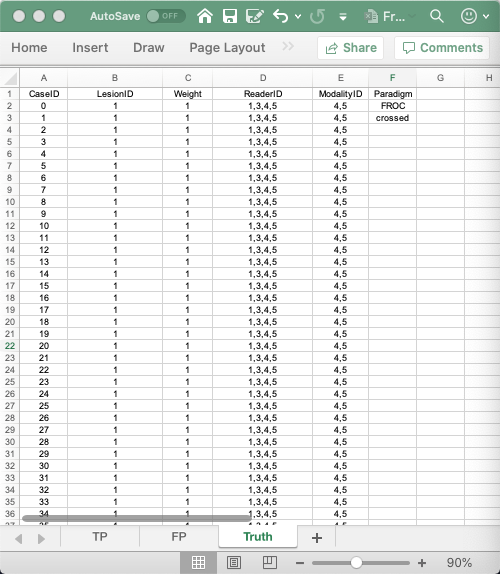
\includegraphics[width=0.5\linewidth,height=0.2\textheight]{images/frocData} 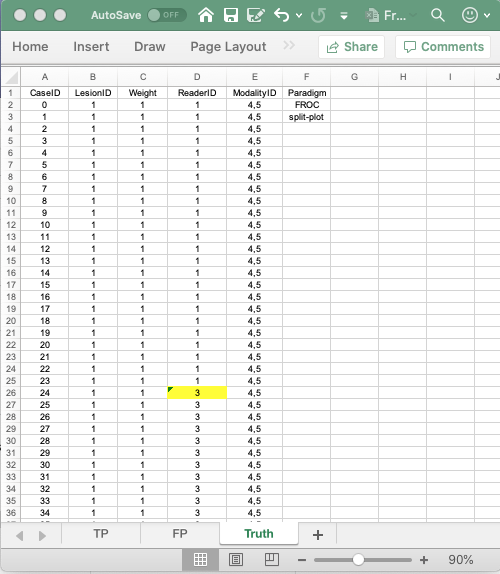
\includegraphics[width=0.5\linewidth,height=0.2\textheight]{images/frocDataSpVaryK1K2} 

}

\caption{Truth worksheets; (a) LEFT=FrocData.xlsx, original crossed dataset; (b) RIGHT=FrocDataSpVaryK1K2.xlsx, modified split-plot dataset}\label{fig:frocDataSpVaryK1K2}
\end{figure}

\begin{itemize}
\tightlist
\item
  The above figure shows that the \texttt{ReaderID} column for cases \texttt{0:23} has been replaced with a 1, meaning that only reader 1 interprets these cases in both modalities. This yields 24 abnormal cases for reader 1 in each modality. Normal cases for this reader are \texttt{100:122}.
\item
  Not shown above: \textbf{all interpretations by reader 1 occurring for cases outside of \texttt{0:23} and \texttt{100:122} in the other two worksheets (\texttt{TP} and \texttt{FP}) are deleted}.
\item
  The \texttt{ReaderID} column for cases \texttt{24:49} are replaced by 3, corresponding to the second reader. All interpretations by this reader for cases outside of \texttt{24:49} in the other two worksheets are deleted. Normal cases for this reader are \texttt{123:149} and observations outside of this range in the \texttt{TP} and \texttt{FP} worsheets are deleted.
\item
  The \texttt{ReaderID} column for cases \texttt{51:73} are replaced by 4, corresponding to the third reader. All interpretations by this reader for cases outside of \texttt{51:73} in the other two worksheets are deleted. Normal cases for this reader are \texttt{150:171} and observations outside of this range in the \texttt{TP} and \texttt{FP} worsheets are deleted.
\item
  The \texttt{ReaderID} column for cases \texttt{50} and \texttt{74:79} are replaced by 5, corresponding to the fourth reader. All interpretations by this reader for cases outside of the specified range in the other two worksheets are deleted. Normal cases for this reader are \texttt{172:199} and observations outside of this range in the \texttt{TP} and \texttt{FP} worsheets are deleted.
\item
  The modified file is read by the code chunk below. The read function explicitly tests that observations outside of the specified ranges in the \texttt{Truth} sheet are not present in the other two worksheets.
\end{itemize}

\hypertarget{example-of-deletion-of-interpretations}{%
\section{Example of deletion of interpretations}\label{example-of-deletion-of-interpretations}}

\begin{figure}

{\centering 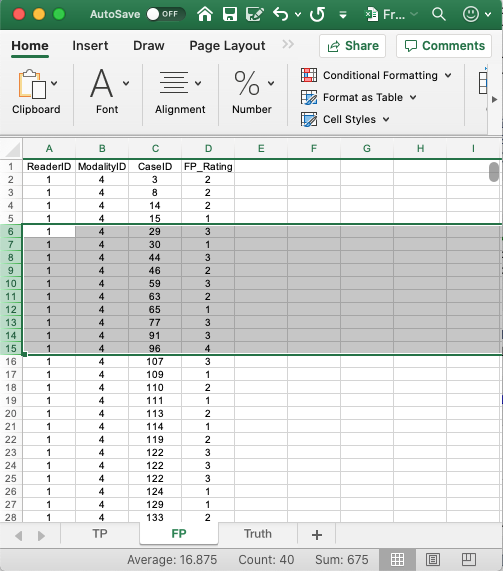
\includegraphics[width=0.5\linewidth,height=0.2\textheight]{images/frocDataFP} 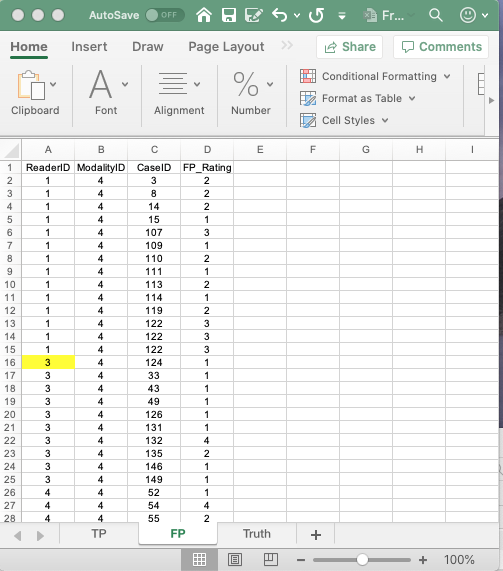
\includegraphics[width=0.5\linewidth,height=0.2\textheight]{images/frocDataSpVaryK1K2FP} 

}

\caption{FP worksheets; (a) LEFT=FrocDataFP.xlsx, original crossed dataset; (b) RIGHT=FrocDataSpVaryK1K2FP.xlsx, modified split-plot dataset}\label{fig:frocDataSpVaryK1K2FP}
\end{figure}

\begin{itemize}
\tightlist
\item
  The two figures above illustrate deletion of interpretations.
\item
  The left panel shows the \texttt{FP} worksheet for the original crossed data.
\item
  For reader 1 and modality 4 it contains cases 29, 30, 44, \ldots{}, 91, 96 that do not belong to the split-plot dataset for this reader.
\item
  Specifically, they are outside of \texttt{0:23} and \texttt{100:122}, the allowed ranges for this reader.
\item
  These are deleted, see right panel of above figure. The next allowed cases for this reader are \texttt{107,\ 109,....,\ 122}.
\item
  The procedure is repeated for all readers and both \texttt{TP} and \texttt{FP} sheets.
\end{itemize}

\begin{Shaded}
\begin{Highlighting}[]
\NormalTok{fedsp <-}\StringTok{ }\KeywordTok{system.file}\NormalTok{(}\StringTok{"extdata"}\NormalTok{, }\StringTok{"toyFiles/FROC/FrocDataSpVaryK1K2.xlsx"}\NormalTok{,}
                       \DataTypeTok{package =} \StringTok{"RJafroc"}\NormalTok{, }\DataTypeTok{mustWork =} \OtherTok{TRUE}\NormalTok{)}
\NormalTok{x2 <-}\StringTok{ }\KeywordTok{DfReadDataFile}\NormalTok{(fedsp, }\DataTypeTok{newExcelFileFormat =} \OtherTok{TRUE}\NormalTok{)}
\NormalTok{t2 <-}\StringTok{ }\NormalTok{x2}\OperatorTok{$}\NormalTok{truthTableStr}
\end{Highlighting}
\end{Shaded}

\hypertarget{understanding-truthtablestr-object-t2}{%
\section{\texorpdfstring{Understanding \texttt{truthTableStr} object \texttt{t2}}{Understanding truthTableStr object t2}}\label{understanding-truthtablestr-object-t2}}

\begin{itemize}
\tightlist
\item
  The following line below yields 46 (= 2x23) as reader 1 (second subscript) provides interpretations in both modalities (first subscript is blank) for all normal cases (third subscript is 1:100 and fourth subscript is 1) and there are 23 normal cases interpreted by reader 1.
\end{itemize}

\begin{Shaded}
\begin{Highlighting}[]
\KeywordTok{sum}\NormalTok{(}\OperatorTok{!}\KeywordTok{is.na}\NormalTok{(t2[,}\DecValTok{1}\NormalTok{,}\DecValTok{1}\OperatorTok{:}\DecValTok{100}\NormalTok{,}\DecValTok{1}\NormalTok{]))}
\CommentTok{#> [1] 46}
\end{Highlighting}
\end{Shaded}

\begin{itemize}
\tightlist
\item
  The following line confirms the first line, with a 1 contribution coming from each case in range 1:23.
\end{itemize}

\begin{Shaded}
\begin{Highlighting}[]
\KeywordTok{sum}\NormalTok{(}\OperatorTok{!}\KeywordTok{is.na}\NormalTok{(t2[,}\DecValTok{1}\NormalTok{,}\DecValTok{1}\OperatorTok{:}\DecValTok{23}\NormalTok{,}\DecValTok{1}\NormalTok{]))}
\CommentTok{#> [1] 46}
\end{Highlighting}
\end{Shaded}

\begin{itemize}
\tightlist
\item
  The following line yields 48 (= 2x24) because the fourth subscript (2) applies to abnormal cases with at least one lesion, and we know that this reader has interpreted 24 abnormal cases.
\end{itemize}

\begin{Shaded}
\begin{Highlighting}[]
\KeywordTok{sum}\NormalTok{(}\OperatorTok{!}\KeywordTok{is.na}\NormalTok{(t2[,}\DecValTok{1}\NormalTok{,}\DecValTok{101}\OperatorTok{:}\DecValTok{124}\NormalTok{,}\DecValTok{2}\NormalTok{]))}
\CommentTok{#> [1] 48}
\end{Highlighting}
\end{Shaded}

\begin{itemize}
\tightlist
\item
  The following line yields 54 (= 2x27) because the fourth subscript (1) applies to normal cases and we know that reader 2 has interpreted 27 normal cases.
\end{itemize}

\begin{Shaded}
\begin{Highlighting}[]
\KeywordTok{sum}\NormalTok{(}\OperatorTok{!}\KeywordTok{is.na}\NormalTok{(t2[,}\DecValTok{2}\NormalTok{,,}\DecValTok{1}\NormalTok{]))}
\CommentTok{#> [1] 54}
\end{Highlighting}
\end{Shaded}

\begin{itemize}
\tightlist
\item
  The following line yields 52 (= 2x26) because the fourth subscript (2:4) applies to abnormal cases with at least one lesion, and we know that reader 2 has interpreted 26 abnormal cases.
\end{itemize}

\begin{Shaded}
\begin{Highlighting}[]
\KeywordTok{sum}\NormalTok{(}\OperatorTok{!}\KeywordTok{is.na}\NormalTok{(t2[,}\DecValTok{2}\NormalTok{,,}\DecValTok{2}\OperatorTok{:}\DecValTok{4}\NormalTok{]))}
\CommentTok{#> [1] 52}
\end{Highlighting}
\end{Shaded}

\hypertarget{references-9}{%
\section{References}\label{references-9}}

\bibliography{packages.bib,myRefs.bib}

\end{document}
